\chapter{Dispersed-phase simulations in liquid JICF}
	\label{ch6:jicf_lgs_simulations}


%Describe here all our results from the lagrangian simulations:
%
%\begin{itemize}
%
%	\item Effects of applying full workflow: w/wo ALM, w/wo secondary atomization ...
%	
%	\item Mesh convergence study: specify it
%	
%	\item Validation with experiments
%	
%	\item Mass conservation issues: lagrangian tracking, etc. 
%	
%
%\end{itemize}


\section{Introduction}

This chapter presents results from lagrangian simulations performed with the SLI models described in Chapter \ref{ch4:sli_development}. The test case used is the academic JICF of \citeColor[becker_breakup_2002], for which resolved simulations of the atomization process were detailed in Chapter \ref{ch5:jicf_resolved_simulations}. Data for these computations are used to build the injectors in order to run dispersed phase simulations in the same configuration, which are shown to be less computationally expensive than the resolved ones. \hl{...}


\section{Computational setup}

The geometry replicating the experimental test bench is the same than the one used for the resolved simulations, depicted in Figure \ref{fig:numerical_setup_maquette_JICF_DLR}. The operating points simulated are the ones from Table \ref{tab:jicf_operating_conditions}. Regarding the mesh employed, it was shown in $\S$\ref{sec:ch5_initial_conditions} that an element size of $\Delta x = 0.5$ mm allows to transport the estimated turbulence in these cases. Nevertheless, the simulations from Chapter \ref{ch5:jicf_resolved_simulations} use a mesh with this cell size only inside the plenum upstream and around the injector, while downstream the injector the mesh size is enlarged as there is no liquid at this region. This mesh was shown in Figure \ref{fig:jicf_dlr_mesh}. In the lagrangian simulations performed in this chapter, injection is performed at the sampling planes downstream the injector seen in Figure \ref{fig:jicf_IBs_sketch_discretization}, and the region of interest extends up to a location at $x = 80$ mm downstream the injector, which corresponds to the location where the experiments from \citeColor[becker_breakup_2002] report results on fluxes and SMD. Therefore, lagrangian simulations use a baseline cell size of $\Delta x = 0.5$ mm in the plenum from the gaseous inlet up to $x = 85$ mm downstream the injector in order to allow for turbulent transport up to the experimental validation plane (located at $x = 80$ mm). The mesh used, shown in Figure \ref{fig:jicf_dlr_mesh_LGS}, is composed of $74 \cdot 10^6$ elements, being therefore heavier than the baseline mesh employed for the resolved simulations but eventually lighter due to the lack of AMR (see the increase of element size in the resolved simulations at Figure \ref{fig:JICF_nelem_increase_t_0_to_2}, which shows that the smallest mesh obtained for a established jet contains $200 \cdot 10^6$ elements). Liquid particles are injected in this mesh as lagrangian point-particles whose dynamics follow the equations from  $\S$\ref{sec:ch3_EL_formalisms}. The energy equation is not considered since the test bench is at ambient temperature and evaporation does not take place.

\clearpage


%The geometry replicating the experimental test bench is the same than the one used for the resolved simulations, depicted in Figure \ref{fig:numerical_setup_maquette_JICF_DLR}. The operating points simulated are the ones from Table \ref{tab:jicf_operating_conditions}. Regarding the mesh employed, it was shown in $\S$\ref{sec:ch5_initial_conditions} that an element size of $\Delta x = 0.5$ mm allows to transport the estimated turbulence in these cases. Nevertheless, the simulations from Chapter \ref{ch5:jicf_resolved_simulations} use a mesh with this cell size only inside the plenum upstream and around the injector, while downstream the injector the mesh size is enlarged as there is no liquid at this region. This mesh was shown in Figure \ref{fig:jicf_dlr_mesh}. In the lagrangian simulations performed in this chapter, injection is performed at the sampling planes downstream the injector seen in Figure \ref{fig:jicf_IBs_sketch_discretization}, and the region of interest extends up to a location at $x = 80$ mm downstream the injector, which corresponds to the location where the experiments from \citeColor[becker_breakup_2002] report results on fluxes and SMD. Therefore, lagrangian simulations use a baseline cell size of $\Delta x = 0.5$ mm in the plenum from the gaseous inlet up to $x = 85$ mm downstream the injector. Furthermore, the mesh is refined \hl{in the region immediately downstream the injection nozzle to} $\Delta x = 0.3$ mm to allow for a better resolution of the gaseous field perturbed by the ALM, as the turbulent structures from the resolved simulations reported in $\S$\ref{ch5:subsec_turbulent_structures_in_gaseous_field} have smaller characteristic sizes than the turbulence further upstream. It is, however, worth to keep in mind that the gaseous field close to the interface was refined in the resolved simulations to the interface mesh size, allowing for a better resolution of turbulence. This refinement is not available in the dispersed phase simulations, therefore the refinement to $\Delta x = 0.3$ mm. The mesh used, shown in Figure \ref{fig:jicf_dlr_mesh_LGS}, is composed of \textbf{XX} elements, being therefore larger than the baseline mesh employed for the resolved simulations but eventually cheaper due to the lack of AMR, as simulations. Liquid particles are injected in this mesh as lagrangian point-particles whose dynamics follow the equations from  $\S$\ref{sec:ch3_EL_formalisms}. The energy equation is not considered since the test bench is at ambient temperature and evaporation does not take place.

\begin{figure}[h!]
	\centering
	\includeinkscape[inkscapelatex=false,scale=0.8]{./part2_developments/figures_ch6_lagrangian_JICF/jicf_mesh_LGS}
	\caption{Mesh employed for dispersed-phase simulations of the full configuration from Figure \ref{fig:numerical_setup_maquette_JICF_DLR}}
	\label{fig:jicf_dlr_mesh_LGS}
\end{figure}


%\section{Evaporation phenomena}
%
%\textbf{Note: this analysis could perfectly be in the previous chapter}.
%
%As indicated in Table \ref{tab:jicf_operating_conditions}, the temperatures of both liquid kerosene and gaseous air are low (290 and 288 K respectively) and there is not direct evaporation of fuel. Nevertheless, some evaporation can occur at ambient temperature if the vapour pressure of the liquid is lower than the ambient pressure. In the experiments, the ambient pressure is $p_g = 6$ bar, while the vapour pressure of kerosene at $288$ K is $p_{vap} = 0.003$ bar \citepColor[shepherd_flash_2000]. Therefore, evaporation might be possible.
%
%It is tested that ... Two characteristic times are used in the low We case (since the lowest velocity is found there, and the droplets take more time to reach the validation plane at 80 mm)/
%
%\begin{itemize}
%
%	\item The time that a droplet takes to reach the plane x = 80 mm. From the SPS results in $\S$\textbf{??} (or Table \textbf{??}), the first droplets at x = 10 mm are obtained at $t_{resolv} = 0.3$ ms after injection. Then, the first droplets injected at this location in the lagrangian simulations reach the validation plane after $t_\mathrm{lagr} = $ ms. Hence, a characteristic time defined as the :
%	
%	\begin{equation}
%	\tau_{validation} = t_{resolv}  + t_\mathrm{lagr}
%	\end{equation}
%	
%	\item Evaporation time rate is used by means of the $d^2$ law. This law that the square of the droplet's diameter diminishes linearly with time:
%	
%	\begin{equation}
%	\label{eq:d2_law}
%	d^2 \left( \right) = d_0^2 - K t
%	\end{equation}
%	
%	
%	where $K$ is the evaporation rate and $d_0$ the initial diameter of the droplet. The value K ... (see 2006 Ghassemi).
%	
%	
%	\text{NAH}. The evolution in diameter after a given time $t$ can then be obtained as:
%	
%	\begin{equation}
%	\Delta d^2 = d_0^2 - d^2 \left( \right) = K t
%	\end{equation}
%	
%
%\end{itemize}

\section{Experimental results from literature}
\label{sec:ch6_experimental_results}

The study from \citeColor[becker_breakup_2002] reports results on the droplets average size SMD and the liquid volume fluxes in the plane $x = 80$  mm perpendicular to the crossflow. In the resolved simulations of Chapter \ref{ch5:jicf_resolved_simulations} the liquid spray could not reach this location: the increase in mesh size due to a continuous liquid injection and formation of droplets due to atomizatio yielded computations unfeasible if liquid was allowed to travel too far downstream, and hence the liquid domain was restricted up to $x = 10, 15$ mm for the fine and coarse resolutions respectively. This limitation does not apply in the dispersed phase simulations, which can be transported up to the outlet of the domain due to their lower cost compared to the resolved ones. Therefore, the dispersed phase simulations will be compared to the experimental results presented at 80 mm.

Experiments results from PDA measurements can be found in the articles \citeColor[becker_breakup_2002] and \citeColor[rachner_modelling_2002]. Among those, quantitative maps of SMD and volume flux are given, which are shown in Figure \ref{fig:maps_Becker_expe_results}. For both operating points, the volume flux shows a circumferential pattern where the largest flux is located at the center and is reduced radially. Most of the fuel is then located at the center of the spray plume, which is a common feature in liquid jets in crossflow \citepColor[wu_spray_1998]. The maximum value of volume flux is lower for the low Weber case than in the high Weber one, which is expected since the injected liquid mass flow rate is lower for the former than for the later to keep the same momentum flux ratio $q$ in both cases, as Table \ref{tab:jicf_operating_conditions} shows. Regarding the $SMD$, both maps show a ballistic, layered profile where the largest droplets are located in the top part of the spray. This is due to the higher inertia of the biggest droplets produced, which penetrate further than the smallest ones \citepColor[wu_breakup_1997]. In general, $SMD$ values are larger in the low Weber case since the dynamic pressure (or equivalently, the gaseous velocity) is lower, and the size of the droplets produced were found to be highly dependent on this parameter \citepColor[becker_breakup_2002].


%\begin{figure}[h!]
%\flushleft
%\begin{subfigure}[b]{0.4\textwidth}
%	\centering
%   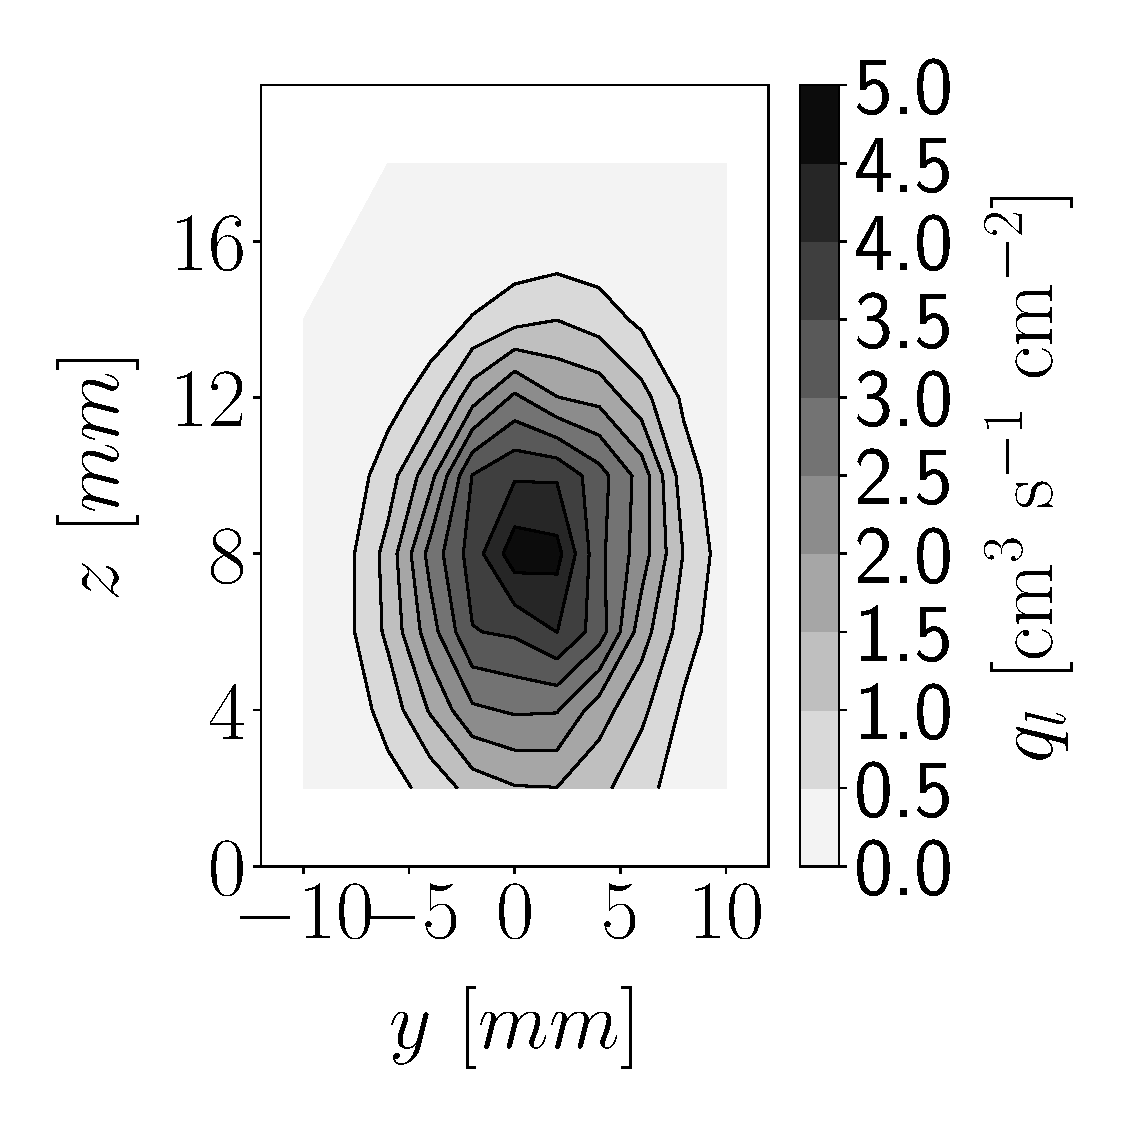
\includegraphics[scale=0.2]{./part2_developments/figures_ch6_lagrangian_JICF/expe_results/map_flux_UG100}
%   \hspace{-0.1in}
%   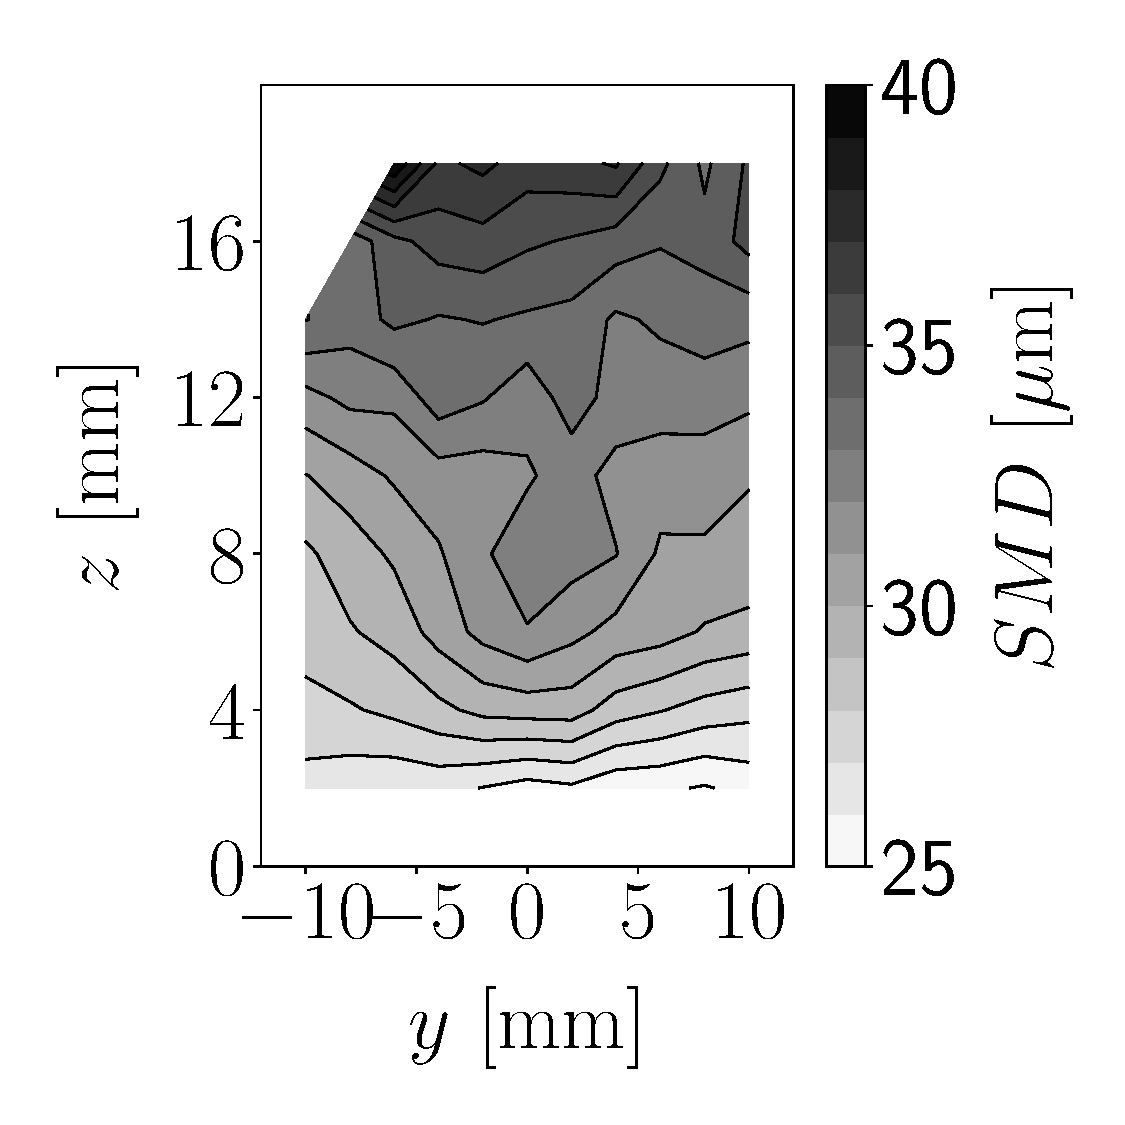
\includegraphics[scale=0.2]{./part2_developments/figures_ch6_lagrangian_JICF/expe_results/map_SMD_UG100}
%   \caption{Low Weber number operating point.}
%   %\label{} 
%\end{subfigure}
%\begin{subfigure}[b]{0.4\textwidth}
%	\flushleft
%   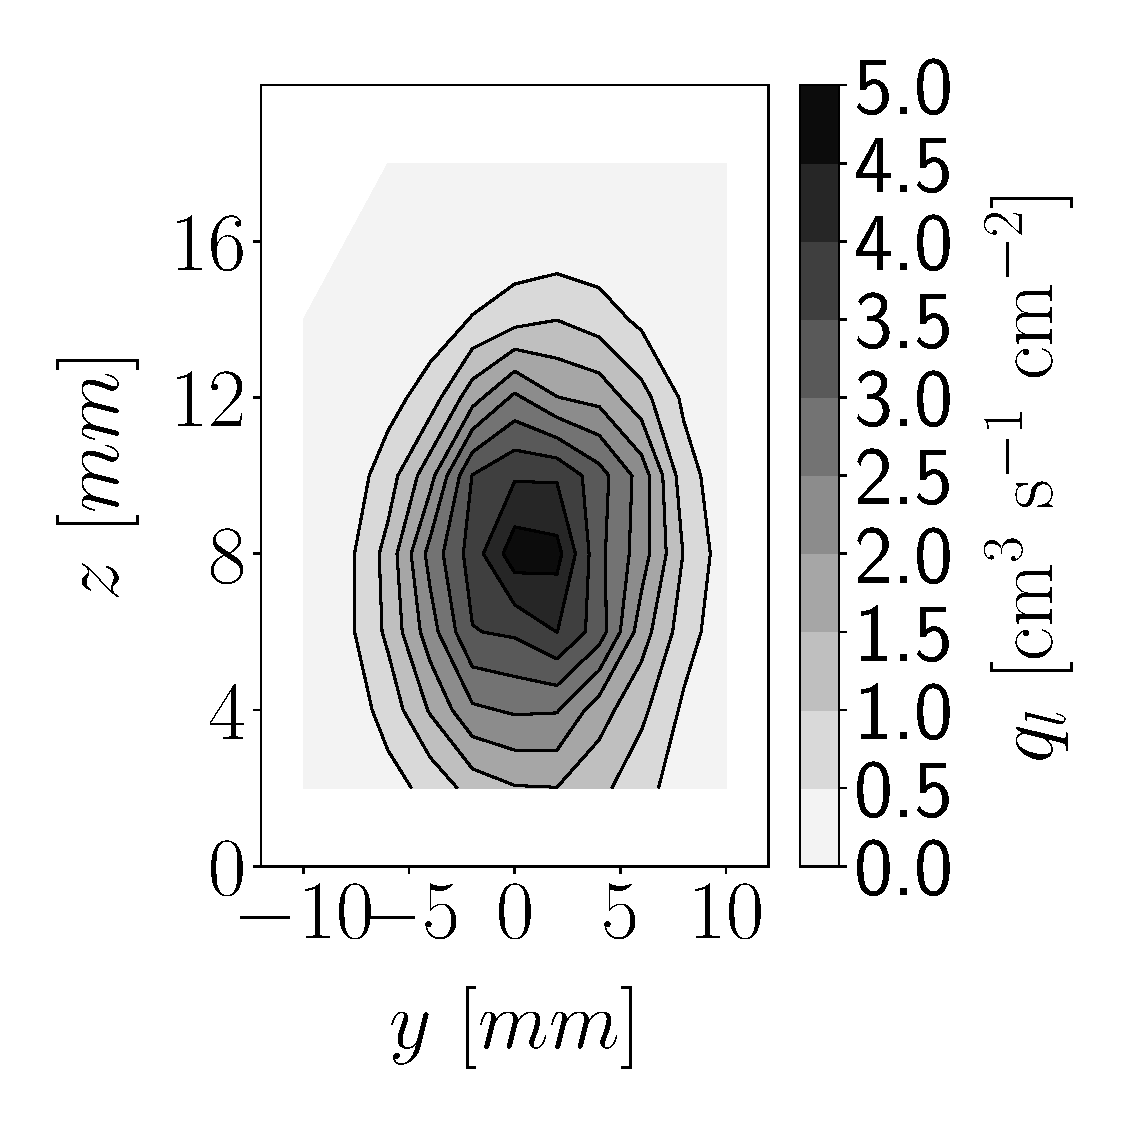
\includegraphics[scale=0.1]{./part2_developments/figures_ch6_lagrangian_JICF/expe_results/map_flux_UG100}
%   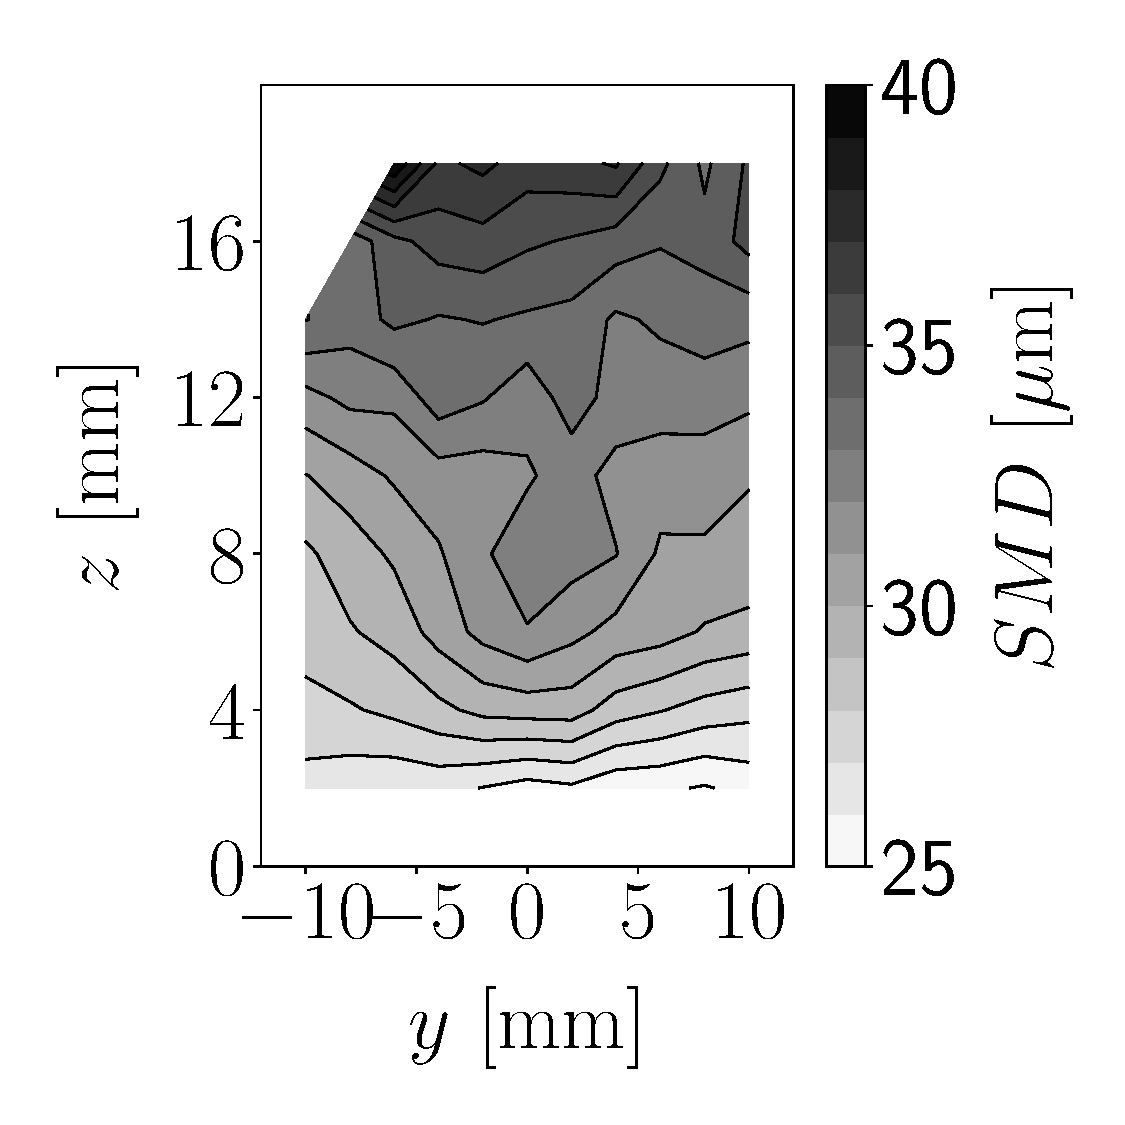
\includegraphics[scale=0.1]{./part2_developments/figures_ch6_lagrangian_JICF/expe_results/map_SMD_UG100}
%   \caption{High Weber number operating point.}
%   %\label{} 
%\end{subfigure}
%\caption{SMD and volume flux maps obtained experimentally by \citeColor[becker_breakup_2002] at a location $x = 80$ mm downstream the liquid injector.}
%\label{fig:maps_Becker_expe_results}
%\end{figure}


%\begin{figure}[h!]
%\flushleft
%\begin{subfigure}[b]{0.45\textwidth}
%	\flushleft
%   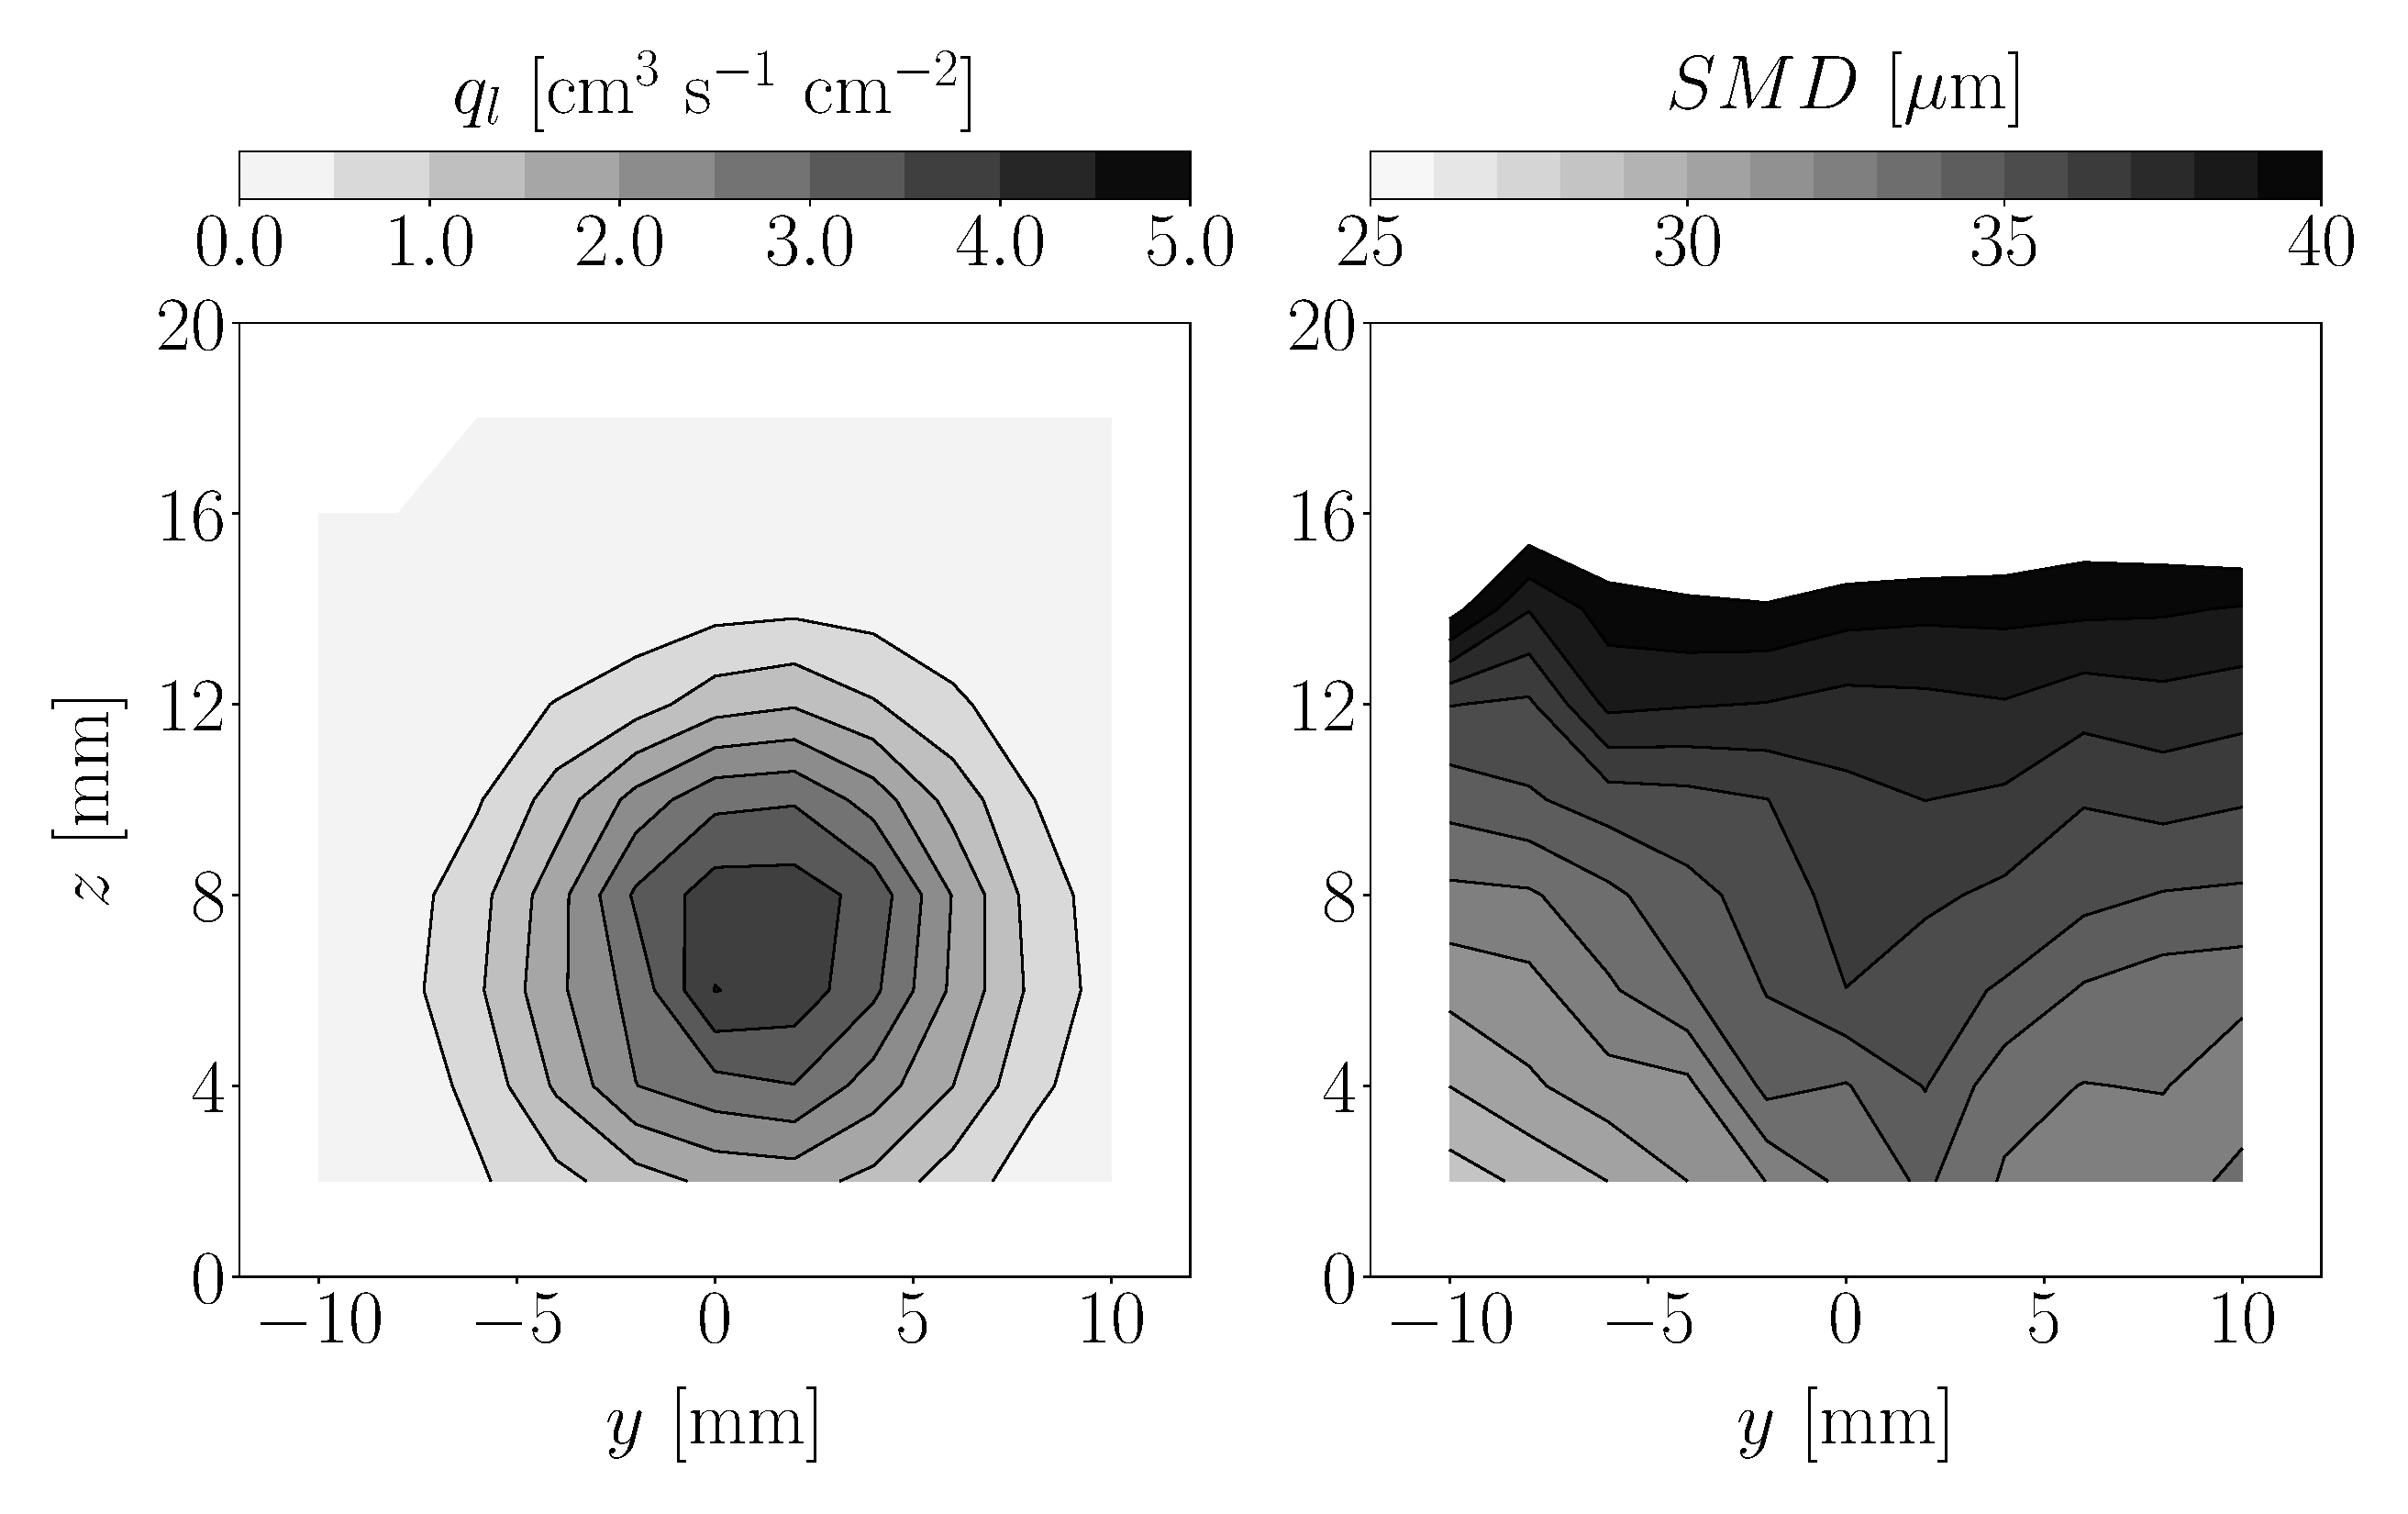
\includegraphics[scale=0.185]{./part2_developments/figures_ch6_lagrangian_JICF/expe_results/maps_UG75}
%   \caption{Low Weber number operating point.}
%   %\label{} 
%\end{subfigure}
%\hspace{0.3in}
%\begin{subfigure}[b]{0.45\textwidth}
%	\centering
%   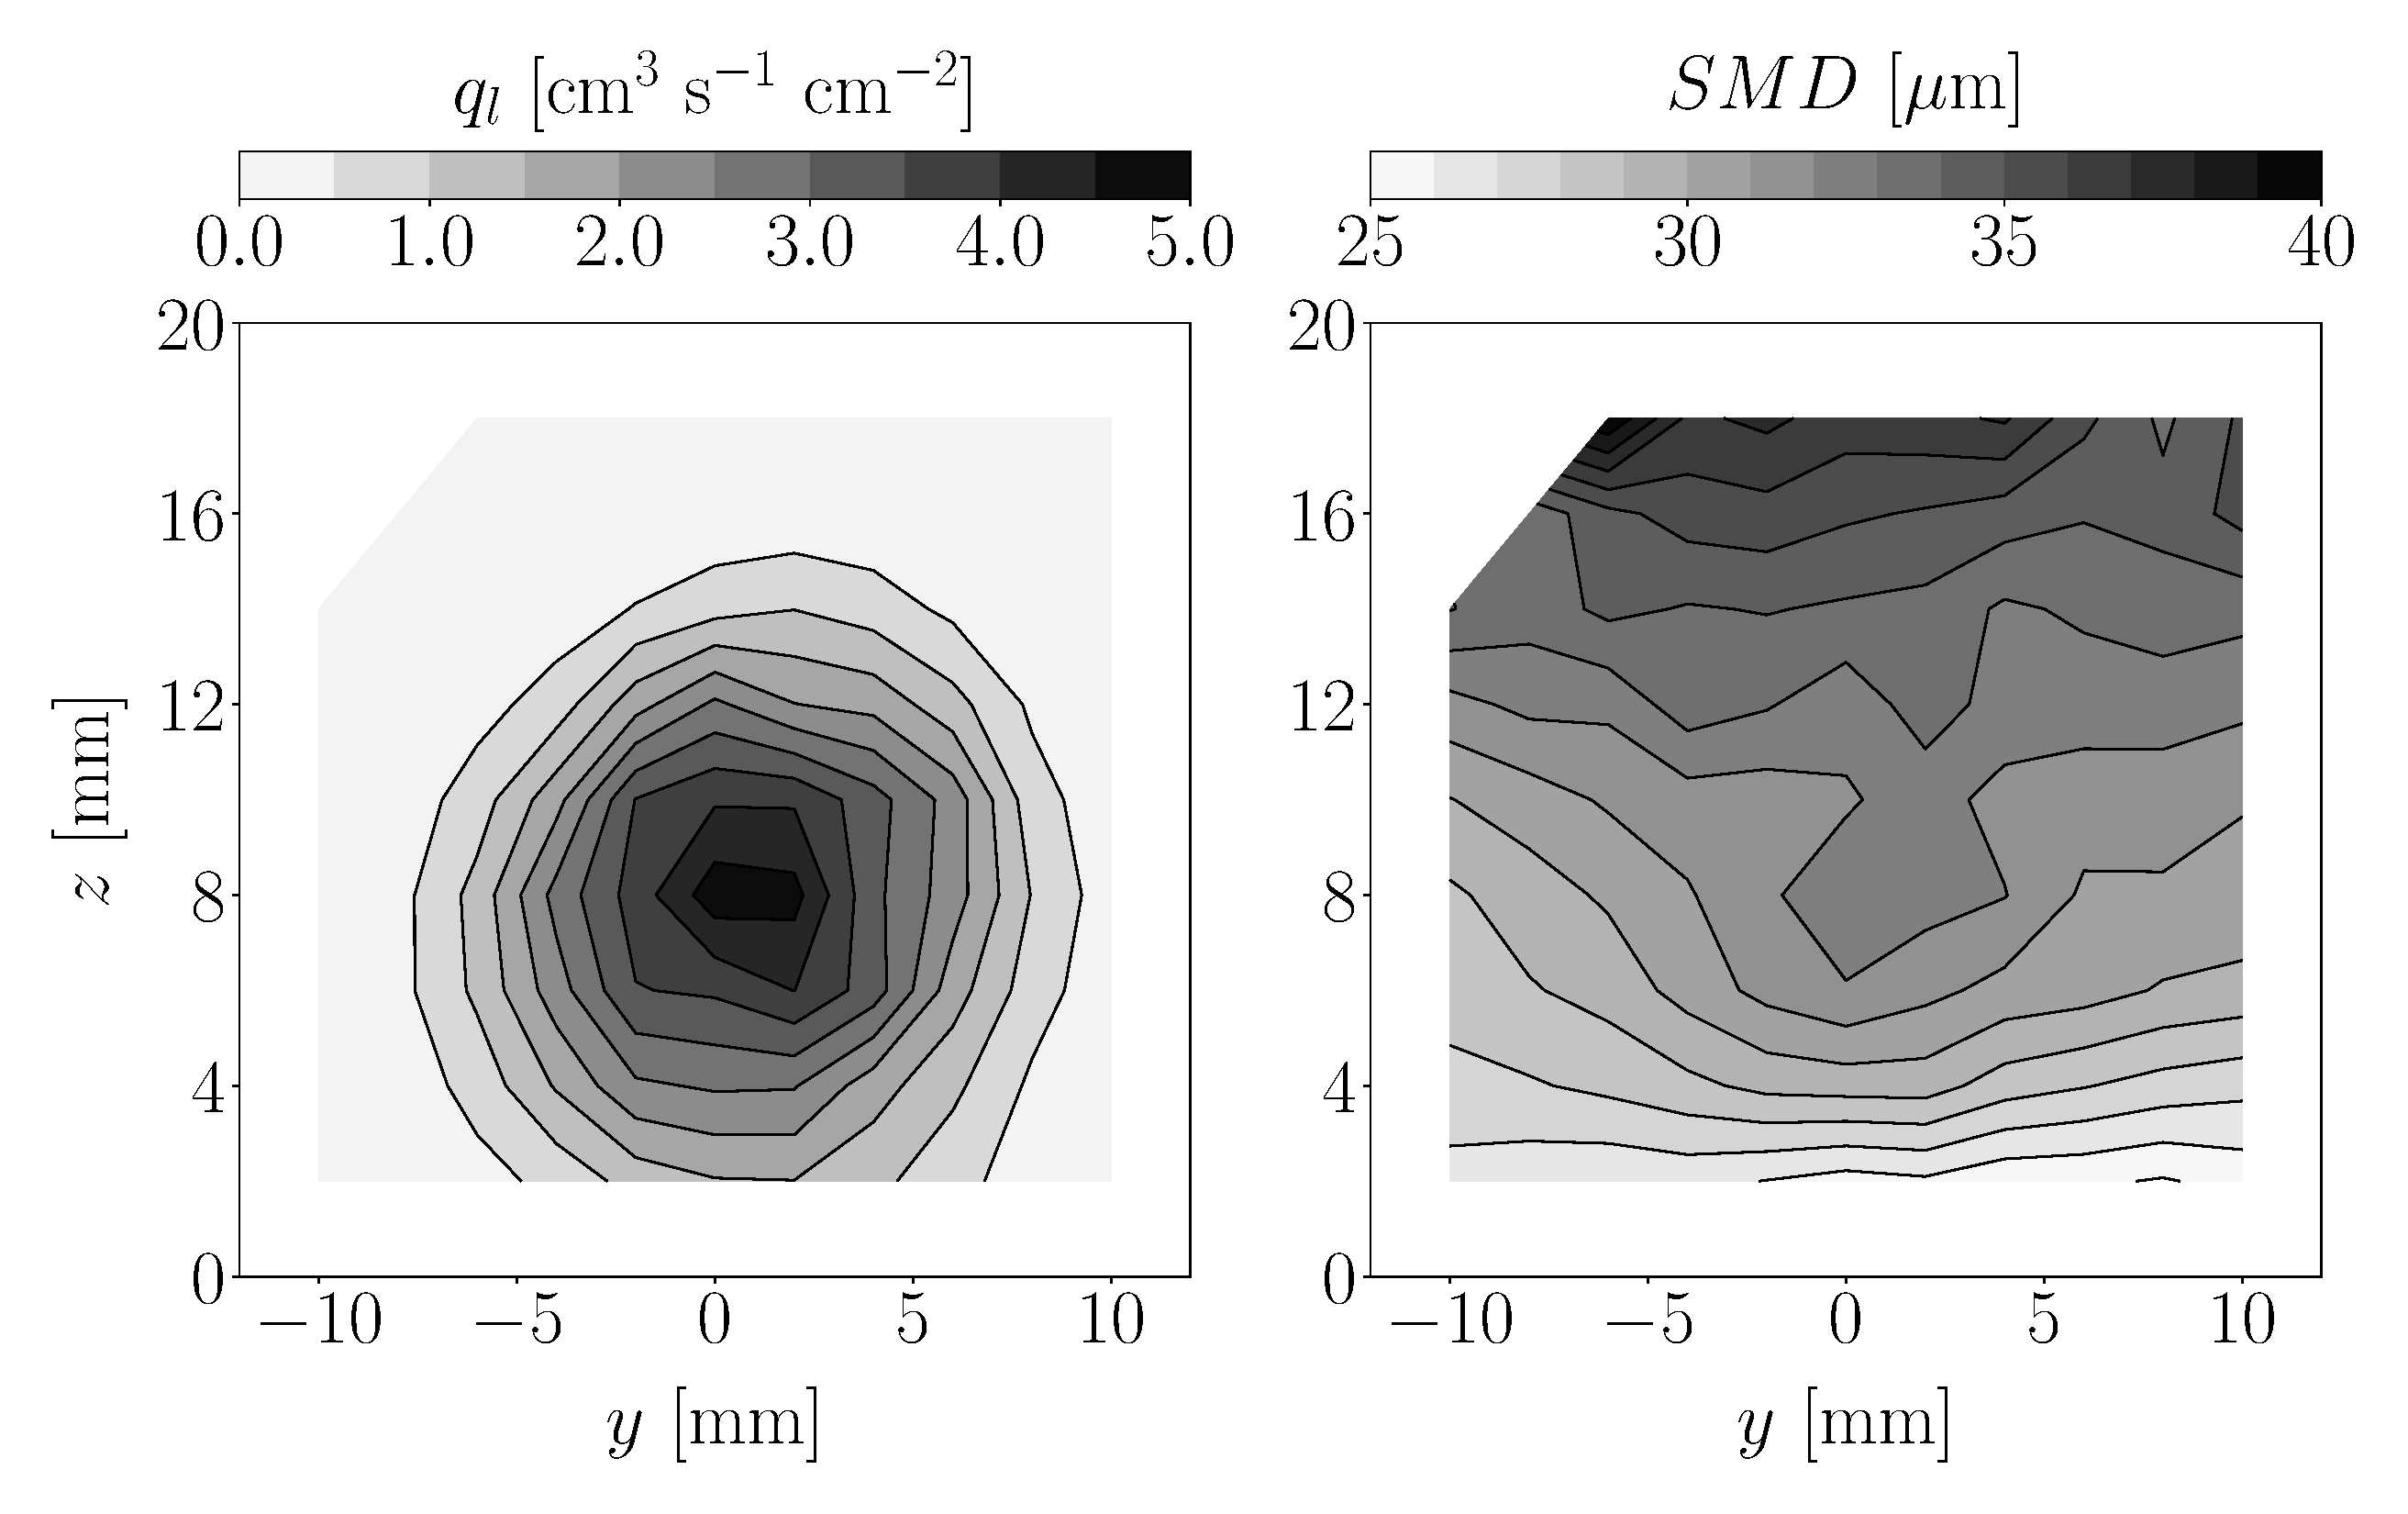
\includegraphics[scale=0.19]{./part2_developments/figures_ch6_lagrangian_JICF/expe_results/maps_UG100}
%   \caption{High Weber number operating point.}
%   %\label{} 
%\end{subfigure}
%\caption{SMD and volume flux maps obtained experimentally by \citeColor[becker_breakup_2002] at a location $x = 80$ mm downstream the liquid injector.}
%\label{fig:maps_Becker_expe_results}
%\end{figure}

\begin{figure}[h!]
\centering
   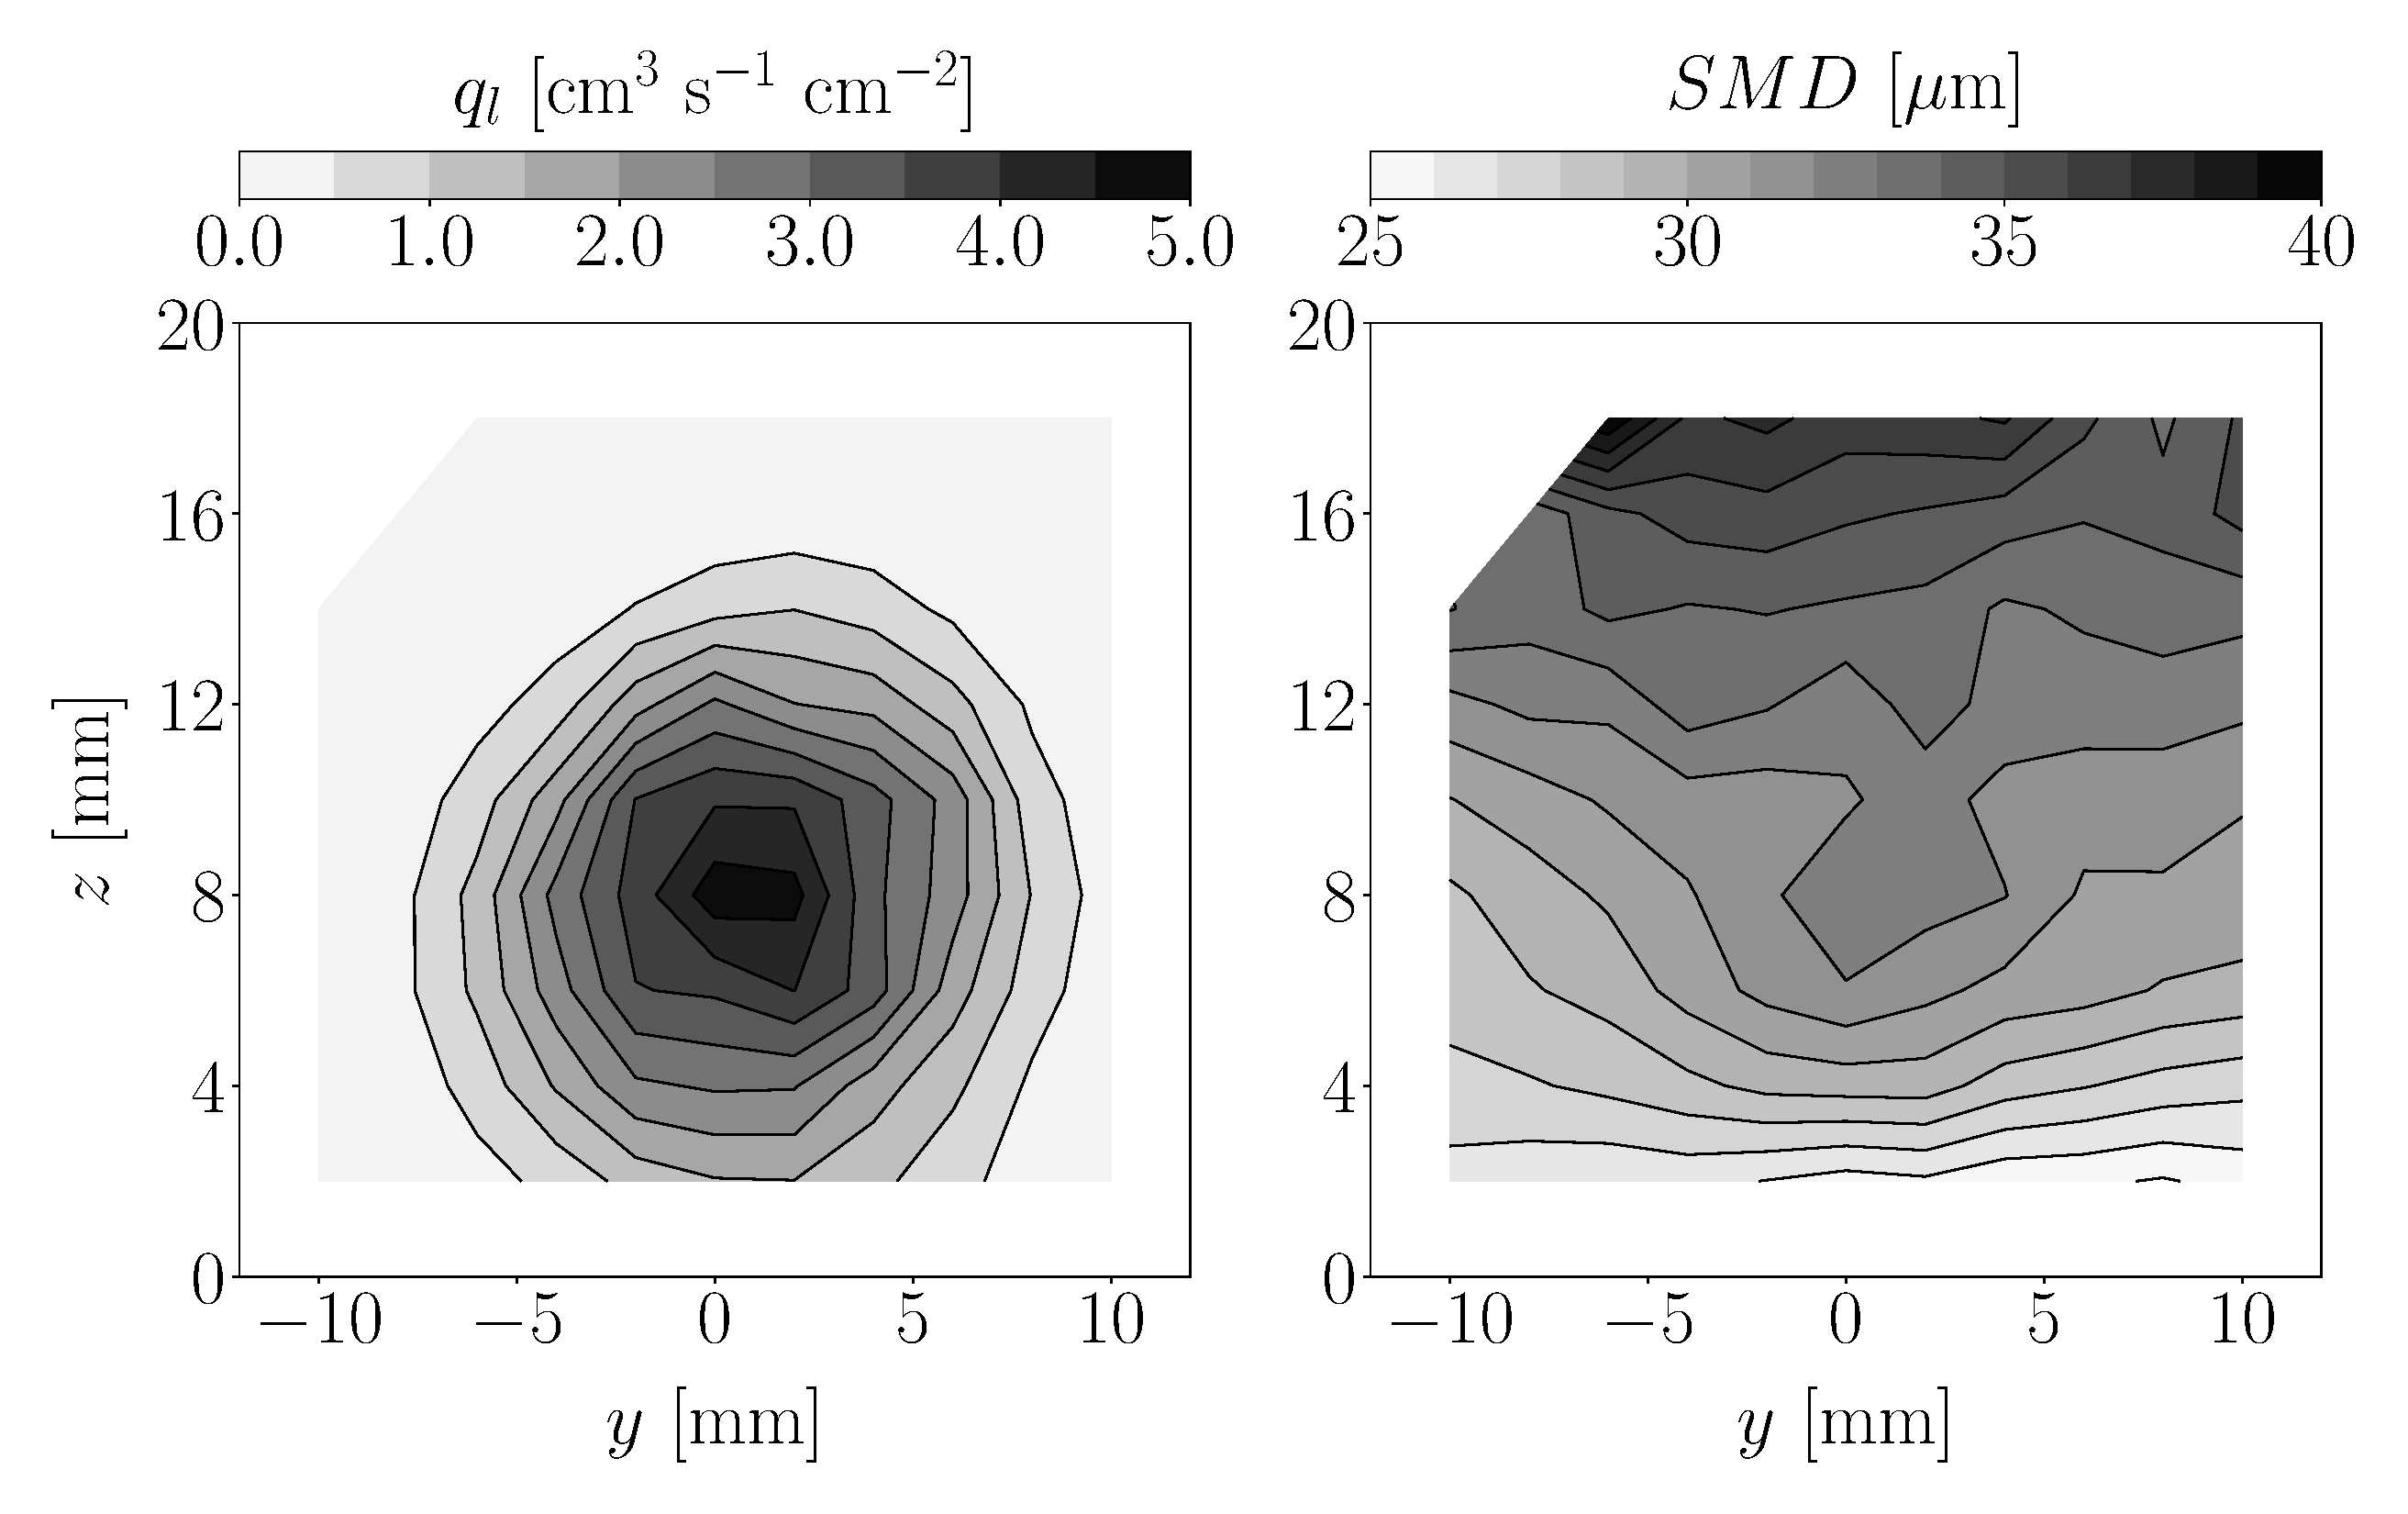
\includegraphics[scale=0.19]{./part2_developments/figures_ch6_lagrangian_JICF/expe_results/maps_UG100}
\caption{SMD and volume flux maps for the high Weber case obtained experimentally by \citeColor[becker_breakup_2002] at a location $x = 80$ mm downstream the liquid injector}
\label{fig:maps_Becker_expe_results}
\end{figure}

Complementary to the maps, qualitative results are also present in the literature which can also be used for validation. These ones are given as the integrated profiles of the liquid volume flux and flux-averaged $SMD$ over the $z$ and $y$ directions, which are then respectively dependent on $y$ and $z$. The equations to obtain such measures are given by Eqs. (\ref{eq:integrated_results_Becker_expe_results}):


\begin{subequations}
\label{eq:integrated_results_Becker_expe_results}
\begin{align}
\langle q_l \left( z \right) \rangle = \frac{1}{L_y} \int_0^{L_y} q_l \left( y, z \right) dy    & ~~~~  ; & \langle SMD \left( z \right) \rangle = \frac{1}{L_y \langle q_l \left( z \right) \rangle} \int_0^{L_y} q_l \left( y, z \right) SMD \left( y, z \right) dy \\
\langle q_l \left( y \right) \rangle = \frac{1}{L_z} \int_0^{L_z} q_l \left( y, z \right) dz    & ~~~~  ; & \langle SMD \left( y \right) \rangle =  \frac{1}{L_z \langle q_l \left( z \right) \rangle} \int_0^{L_z} q_l \left( y, z \right) SMD \left( y, z \right) dz
\end{align}
\end{subequations}


%\begin{equation}
%\langle q_l \left( z \right) \rangle = \frac{1}{L_y} \int_0^{L_y} q_l \left( y, z \right) dy ~~~~; ~~~~ \langle SMD \left( z \right) \rangle = \frac{1}{L_y \langle q_l \left( z \right) \rangle} \int_0^{L_y} q_l \left( y, z \right) SMD \left( y, z \right) dy
%\end{equation}
%
%\begin{equation}
%\langle q_l \left( y \right) \rangle = \frac{1}{L_z} \int_0^{L_z} q_l \left( y, z \right) dz ~~~~; ~~~~ \langle SMD \left( y \right) \rangle = \frac{1}{L_z \langle q_l \left( z \right) \rangle} \int_0^{L_z} q_l \left( y, z \right) SMD \left( y, z \right) dz
%\end{equation}

The application of these equations to the experimental results yield the curves from Figure \ref{fig:integrated_results_Becker_expe_results}. The integrated volume flux over $y$ (Figure \ref{fig:integrated_results_Becker_expe_results_over_y}) shows an increase of the volume flux from the bottom part of the spray (PDA measurements closer to wall, for $z < 2$ mm, could not be performed \citeColor[becker_breakup_2002]) until the spray center, where the maximum flux is reached. Then, the flux decreases with $z$ until there is no more liquid present. Flux values are generally larger for the high $We$ point than for the low $We$ one, and the quantity of liquid extends up to further upstream for the former than for the latter due to its larger liquid velocity at injection. Regarding the SMD profiles, both cases follow a ballistic behaviour. The spray of the high $We$ point contains droplets of larger mean size than the low $We$ one.

With respect to the profiles integrated over $z$ (Figure \ref{fig:integrated_results_Becker_expe_results_over_z}), both SMD and flux lines follow parabollic profiles with the largest values present at $y = 0$, i.e. the coordinate for which the largest fluxes are found. The behaviour of the profiles depending on the operating point follow the same tendencies than in Figure \ref{fig:integrated_results_Becker_expe_results_over_y}: lower fluxes and larger droplets for the low $We$ case.



\begin{figure}[h!]
\flushleft
\begin{subfigure}[b]{0.45\textwidth}
	\flushleft
   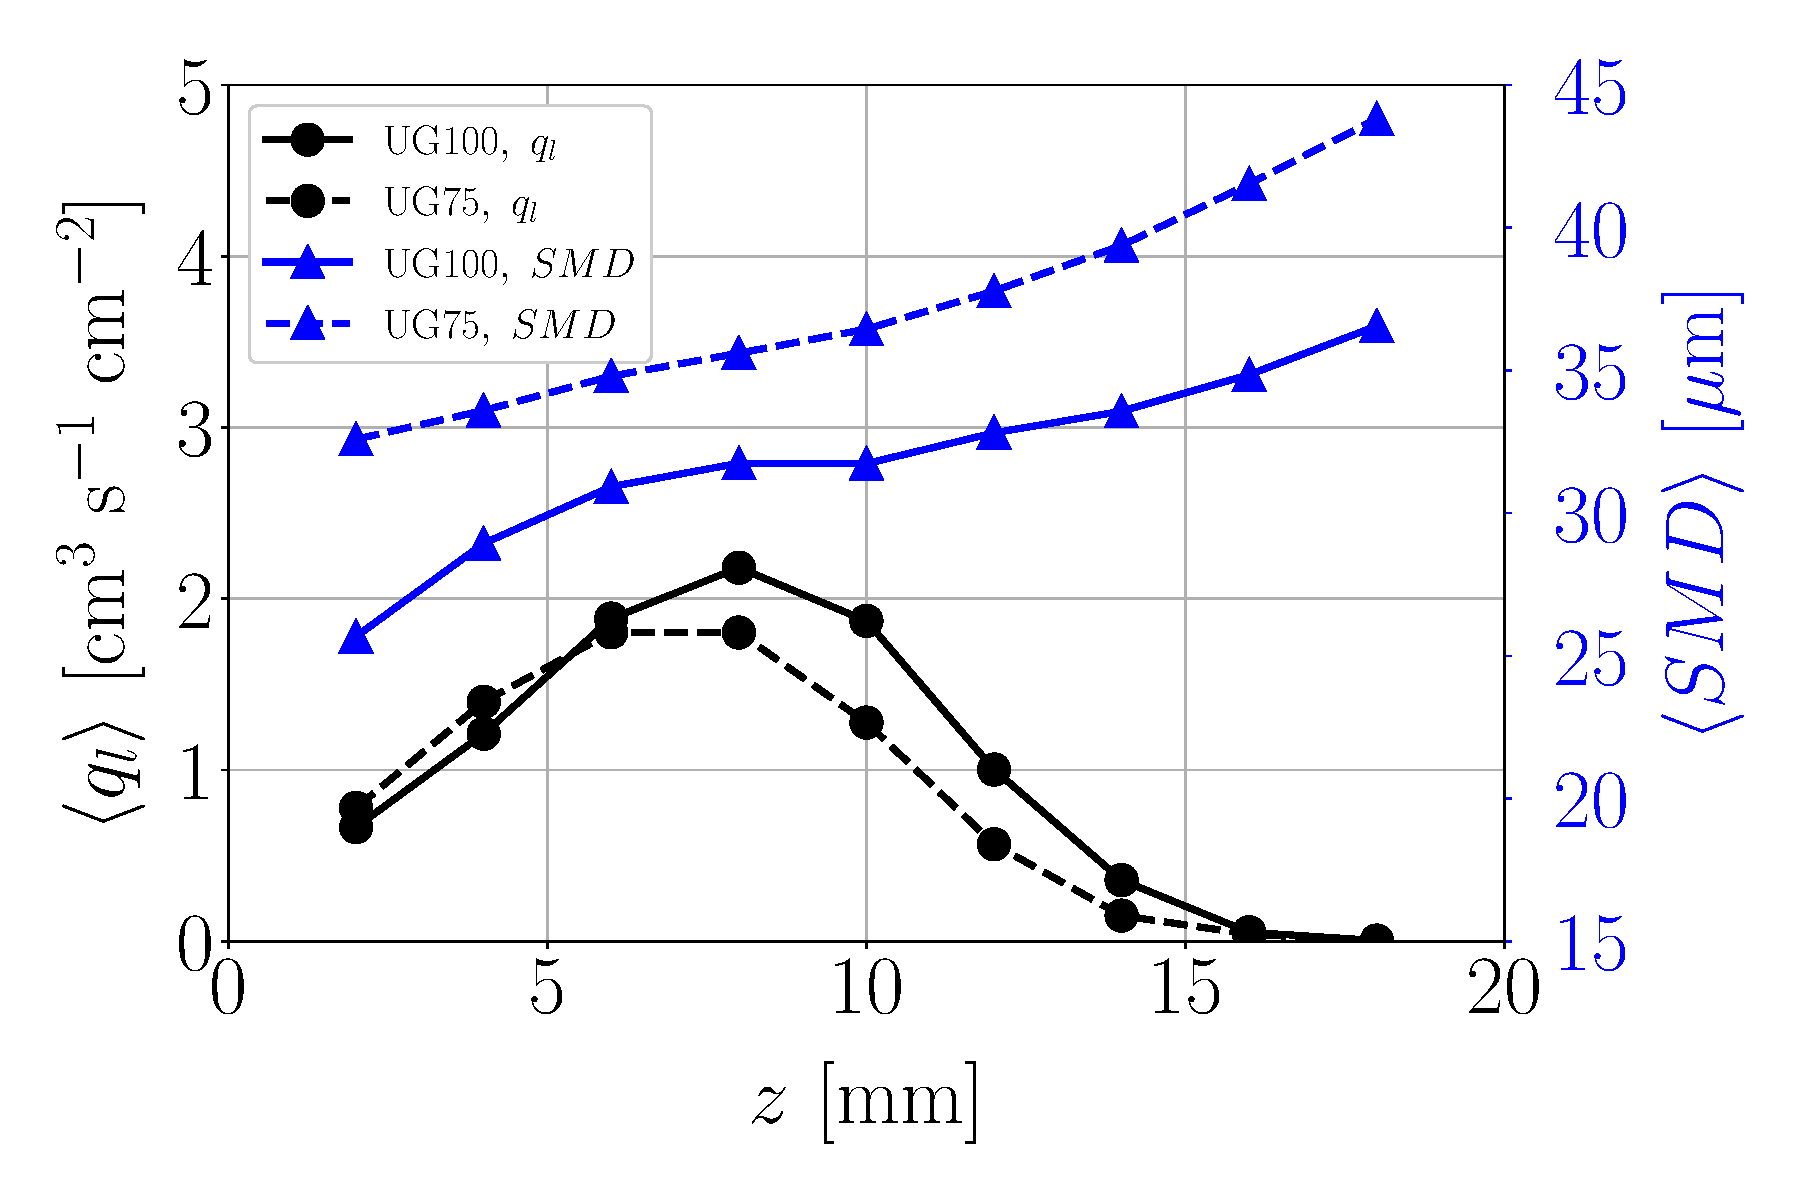
\includegraphics[scale=0.275]{./part2_developments/figures_ch6_lagrangian_JICF/expe_results/integrated_fluxes_along_y}
   \caption{Profiles integrated over $y$.}
  \label{fig:integrated_results_Becker_expe_results_over_y} 
\end{subfigure}
\hspace{0.3in}
\begin{subfigure}[b]{0.45\textwidth}
	\centering
   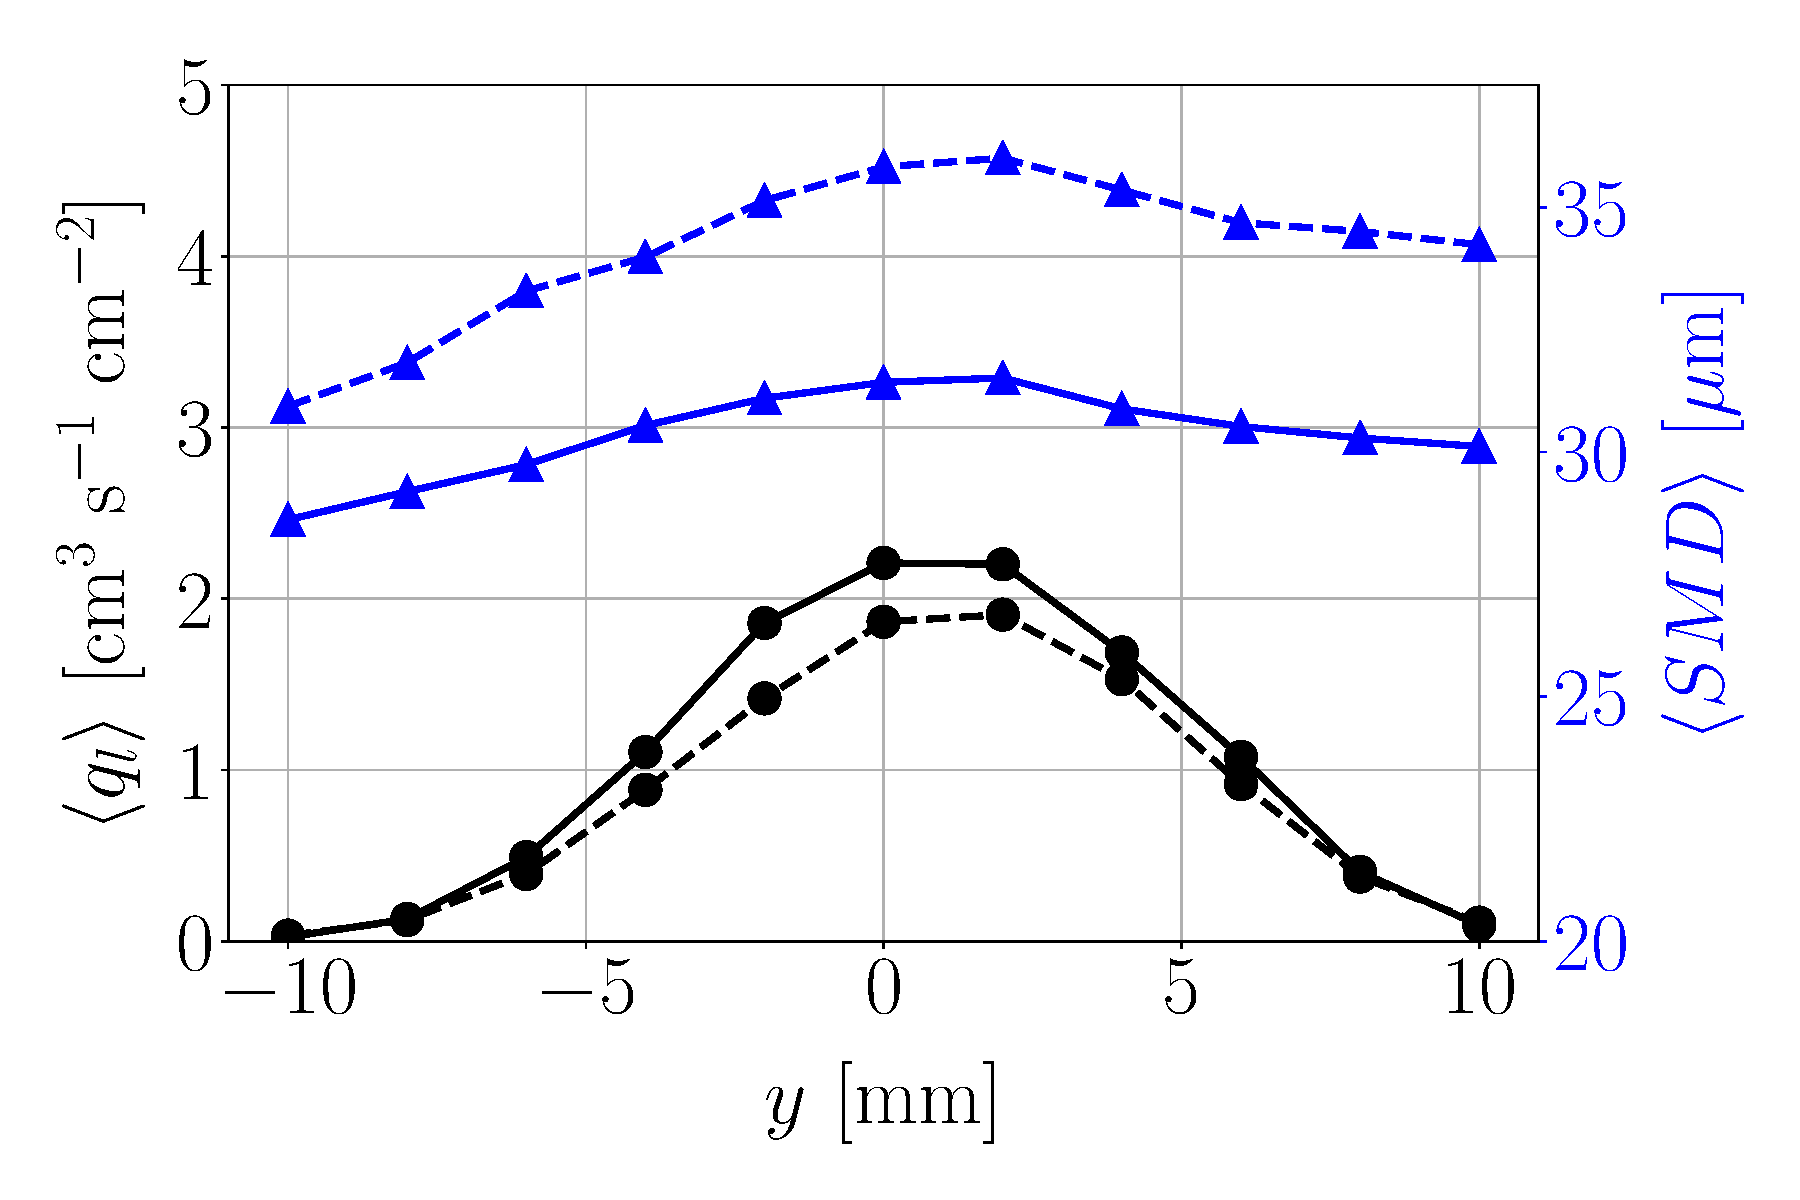
\includegraphics[scale=0.275]{./part2_developments/figures_ch6_lagrangian_JICF/expe_results/integrated_fluxes_along_z}
   \caption{Profiles integrated over $z$.}
  \label{fig:integrated_results_Becker_expe_results_over_z}
\end{subfigure}
\caption[{Integrated liquid volume flux and SMD profiles by \citeColor[becker_breakup_2002] at a location $x = 80$ mm downstream the liquid injector.}]{Integrated liquid volume flux and SMD profiles by \citeColor[becker_breakup_2002] at a location $x = 80$ mm downstream the liquid injector. }
\label{fig:integrated_results_Becker_expe_results}
\end{figure}

\begin{table}[!h]
\centering
\caption{Experimental SMDs at $x = 80$ mm  }
\begin{tabular}{cc}
\thickhline
Operating point & $SMD~\left[ \mu \mathrm{m}\right]$  \\
\thickhline
Low Weber & 31.0  \\  
High Weber & 35.2 \\
\thickhline
\end{tabular}
\label{tab:becker_hassa_SMD_values_sprays}
\end{table}


%\section{Sources of uncertainty in PDA measurements}
\section{Uncertainty in experimental data}
\label{sec:jicf_dlr_experimental_uncertainty}

The experimental results previously shown, obtained by \citeColor[becker_breakup_2002], were obtained through PDA measurements. PDA is one of the most popular experimental techniques to characterize sprays, since it is non-intrusive and provies information on droplets size and velocities which can then be used to also estimate fluxes. It is not, however, exempt of errors, since it is built on the assumption that droplets are spherical and it is well known that PDA measurements yield considerable erros on droplets sizes and fluxes \citepColor[tropea_optical_2011]. Several sources of error have been identified in the past. \citeColor[bachalo_method_1980] explained that optics play a paramount role: the optical setup can lead to detection errors produced by phenomena associated to the misalignment of dual-beam reflected and refracted rays (Gaussian beam Effect) or to the well-known slit effect, which is cause a truncation on the measurement volume through a slit placed so that the droplet volumes to measure can be defined \citepColor[doublet_effet_2019]. Not associated to the actual setup, modifications in the refractive indices of droplets could affect the scattering and yield important errors in particle sizes, specially relevant in multicomponent fuels such as kerosene. The role of the droplet non-sphericity was discussed, stating that PDA is prone to size overestimation when particles are deformed or oscillate in a preferential direction, as also discussed by \citeColor[damaschke_optical_1998]. \citeColor[dullenkopf_comparative_1998] performed PDA measurements on two injectors, a pressure-swirl and an airblast atomizer, and quantified the errors in mass flux by comparing with the results obtained from a patternator. They identified three main sources of error in the flux estimation: the size measurement (which is powered to 3 to calculate the flux, hence increasing exponentially the flux errors), the number count of droplets and the reference area used for measurements (the smaller the area the better, since it can also avoid counting droplets twice). They found that the flux errors on the pressure swirl fluxes were of the order of 10 $\%$, while in the airblast configurations these increased up to 30 $\%$, and also showed that the SMDs could vary up to 30 $\%$ depending on the PDA system used. \citeColor[brandt_experimental_1998] tested an airblast configuration and discussed several possible sources of error in sizes, highlighting the contribution of alignment uncertainties in the setup ($\sim 1~\%$) the change in refractive indices due to heating ($\sim 3.5~\%$) and to deformation of the sampled particles, since accelerated droplets at high velocity environments will be elliptical rather than spherical and the droplets sizes would be overestimated, propagating later the error to the fluxes calculations (this would explain the larger errors found by \citeColor[dullenkopf_comparative_1998] in their airblast atomizer with respect to the pressure-swirl one). In total, uncertainty on dropsizes was quantified to be of 7 $\%$ while the error on fluxes added up to 10 $\%$ if the particles concentration was not too high. It is worth to remark that the test bench of \citeColor[brandt_experimental_1998] is the same one that \citeColor[becker_breakup_2002] used later at DLR to test the liquid kerosene JICF dealt in this theses (even though the atomizer and the operating conditions are different, the PDA systems and optical configurations are equivalent). The experiments from \citeColor[becker_breakup_2002] do not actually provide data on the dropsize uncertainties, but do discuss the errors on mass fluxes and report mean deviations of 20 $\%$ and maximum of 37 $\%$. A posterior study on this configuration was done by \citeColor[becker_experimental_2004], who tested a swirled injector and reported errors on the SMD of $\sim 5 \%$ (no data on fluxes) attributed to optical misalignment and hardware setting. \citeColor[tropea_optical_2011] makes a review on experimental methods involving optical techniques to characterize disperse multiphase flows, and states that PDA measurements often show uncertainted in flux measurements from $20~\%$ up to several hundrers, while errors in particle size often range, in ideal conditions, from 10 to 30 $\%$. 

The objective here is to estimate possible errors in the experimental measurements of \ref{fig:integrated_results_Becker_expe_results} to obtain confidence intervals for validation of numerical results. As mentioned in the previous paragraph, this study gives a mean uncertainty of 20 $\%$ in the fluxes but does not provide data on the diameters. For the same test bench but with different atomizers and operating conditions, \citeColor[brandt_experimental_1998] reports 7 $\%$ and 14 $\%$ of errors for the droplets diameters and fluxes, respectively, while \citeColor[becker_experimental_2004] give SMD uncertainties of $\sim 5 \%$. Even though the PDA setup is identical in the three studies, the provided errors differ among each other, which might be due to the operating conditions, the atomizer or modifications in the optical setup (indeed, \citeColor[doublet_effet_2019] showed through a error propagation analysis that the uncertainties in the diameters were actually spetially sensitive to the elevation angle of the PDA detectors rather than to other parameters). Therefore, in order to estimate the uncertainty of the diameters in the the experimental setup of \citeColor[becker_breakup_2002], it will be assumed that the relation between the dropsizes and fluxes errors is similar as in the study performed in the same testbench (and in similar operating conditions) by \citeColor[brandt_experimental_1998]: errors between fluxes and diameters differ by a factor of 2, which in case of \citeColor[becker_breakup_2002] yields diameter uncertainties of 10 $\%$ since their mean uncertainty for the fluxes is of 20 $\%$. It is important to keep in mind that this estimated error in droplets size is only approximative and could greatly vary in the actual experiments. \\ %Generally, as shown by the previous literature review,  errors in PDA measurements on droplets sizes are not often reported and characteristic 

Since \citeColor[becker_breakup_2002] give values on the flux uncertainties and their experimental data are available, it is possible to estimate the fluxes obtained from the experiments. The flux map ax $x = 80$ mm for the high Weber operating condition together with the grid composed of the probes through which the spray has been sampled is shown in Figure \ref{fig:maps_previous_numerical_results}a. Square probes with 2 mm sides are placed as shown in the figure. Each probe contains a volume flux value $q_l$ which is stored at the center of the probe to plot the maps (as done in the SLI injectors of Figures 
\ref{fig:injectors_sli_uG75_dx10_x05} to \ref{fig:injectors_sli_uG100_dx20_x10_NT}). The grid is then composed of $N_y = 11$ probes in the lateral direction and $N_z = 9$ in the vertical one. Given an arbitrary probe located at a position $\left( j,k \right)$ (where $j$ is the probe index in the lateral direction $y$ and $k$ in the vertical one $z$) with surface $S_\mathrm{j,j}$, the absolute liquid flux through this probe can be calculated by applying Eq. (\ref{eq:ch4_volume_flux_definition}) to the probe volume flux $q_{l{j,k}}$:

\begin{equation}
Q_{l_{j,k}} = q_{l_{j,k}} S_{j,k}
\end{equation}

Then, the total liquid flow rate from the map can be calcuated by adding all the absolute fluxes from each probe:

\begin{equation}
\label{eq:ch6_Ql_total_estimation_from_flux_profiles}
Q_{l} = \sum_{j=1}^{N_y} \sum_{k=1}^{N_z} Q_{l_{j,k}} = \sum_{j=1}^{N_y} \sum_{k=1}^{N_z} q_{l_{j,k}} S_{j,k} = 4062 ~ \mathrm{mm}^3~\mathrm{s}^{-1}
\end{equation}

which, as shown, gives a value of $4062 ~ \mathrm{mm}^3~\mathrm{s}^{-1}$. The injected flow rate for this case is $Q_{l,\mathrm{inj}} = 3710~ \mathrm{mm}^3~\mathrm{s}^{-1}$, as given in Table \ref{tab:jicf_operating_conditions}. Therefore, the PDA measurements report a flux excess with respect to the injected flow rate of $9.5~\%$. This deviation is comprised within the mean uncertainty of $20~\%$ provided by the authors of the experiments. Nevertheless, it is paramount to consider this flux overestimation when comparing with the dispersed-phase simulations performed with SLI, since the liquid rates injected in these ones do not correspond to the experimental flux of $4062 ~ \mathrm{mm}^3~\mathrm{s}^{-1}$ but to the injected one of $Q_{l,\mathrm{inj}} = 3710~ \mathrm{mm}^3~\mathrm{s}^{-1}$. In reality, if the PDA was exempt of errors (which, as explained previously, is never the case), the retrieved experimental flux could not be larger than the injected one as mass is not created in the simulation: and actually, it should be lower since there is filming in the experiments, as shown in Figure \ref{fig:jicf_snapshot_expe_filming}, that reduces the liquid flux perpendicular to the crossflow. The resolved simulations could capture this filming phenomenon in the jet, and the filming flux was quantified in $\S$\ref{sec:ch5_direct_measurement_fluxes_IB}.


\begin{figure}[h!]	
	\centering	
	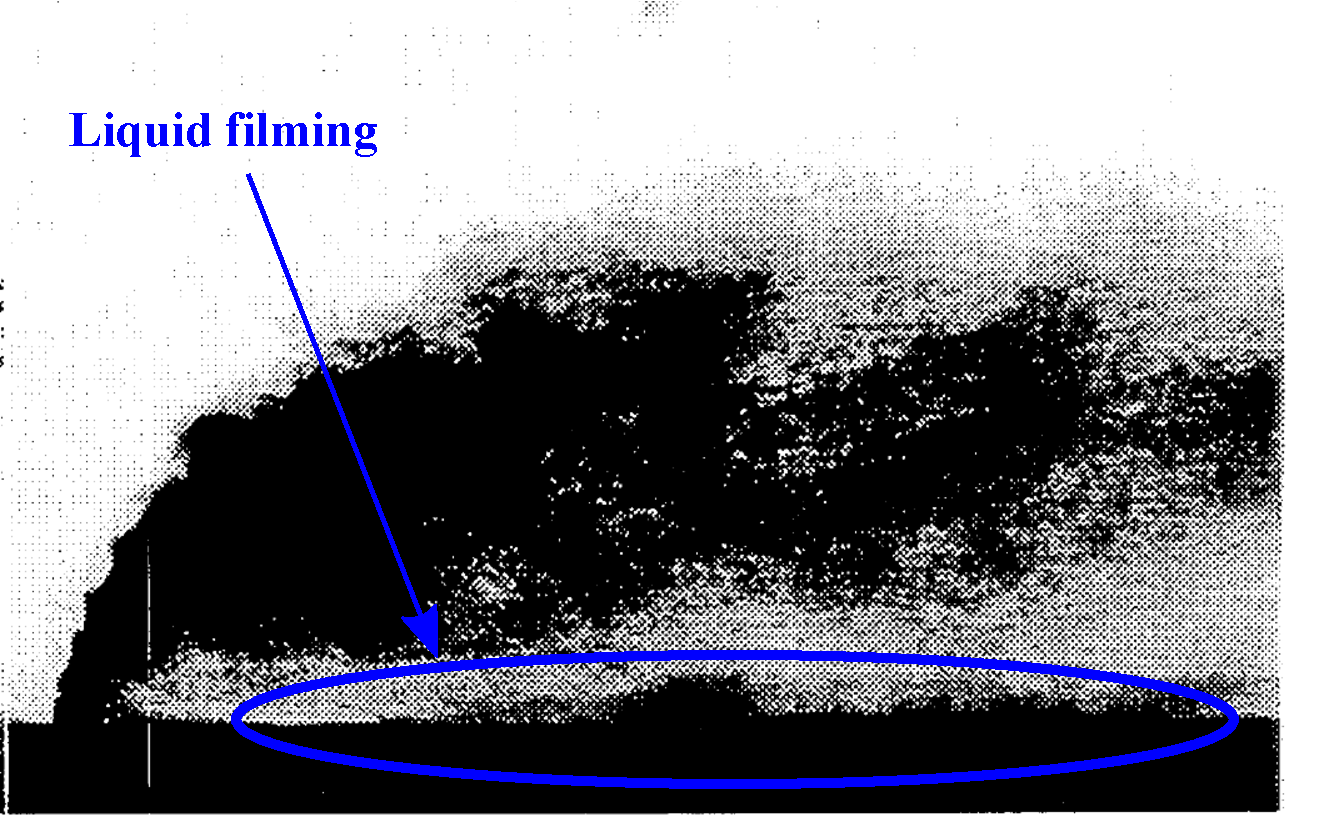
\includegraphics[scale=0.4]{./part2_developments/figures_ch6_lagrangian_JICF/expe_results/snapshot_expe_filming}
	\caption{Snapshot of instantaneous liquid jet from \citeColor[becker_breakup_2002], showing the filming phenomenon}
	\label{fig:jicf_snapshot_expe_filming}
\end{figure}


%snapshot_expe_filming

%\section*{REVIEW on uncertainty: PDA literature}

The work of 1998 paper on ... disclosed errors on the fluxes of 10 $\%$ for a pressure swirl atomizer and of 30 $\%$ for an airblast configuration. Indeed, the experiments of Becker and Hassa report mean errors of 20 $\%$ maximum of 37 $\%$ for liquid fluxes.

PDA present sources of error in:

\begin{itemize}

	\item \textbf{Fluxes}.
	
	\item \textbf{Droplets sizes}. 

\end{itemize}

There are several works that I've obtained dealing with PDA measurement uncertainties. Chronologically:

\begin{itemize}

	\item \textbf{1980 Bachalo} explains that the optical configuration is of particular importance. "\textsl{An error of 10 $\%$ in refractive index results in an error of 10 $\%$ in particle size. For droplets that are deformed in a preferred direction due to, for example, aerodynamic pressure distributions on the droplet, a systematic error in the size measurement could occur}". Hence, if droplets are not spherical the errors can become significant.

	\item \textbf{1998 paper on PDA uncertainties} reports that in previous works (to 1998), errors in fluxes of 100 $\%$ have been reported. Recent efforts (to that date) have been done to minimize such errors. Then, several sources of errors have been identified to arise from the equation used to estimate the flux (put equation somewhere maybe): 1) size measurement due to the third power dependence; 2) umber count depending on the electronics; 3) reference area depending on droplet size, optical configuration and validation scheme. In general, "\textsl{small droplets will not influnce the mass flux significantly so poor detection of small drops should not be a major source of error; however, small droplets sized as large droplets (e.g. slit effect [4]) or large droplets sized as small droplets (trajectory effect [5]) remain problems to be addressed. [...] A final, more subtle, source of error is the alignment and adjustment of the instrument}". This article is also interesting because it compares three different PDA configurations: DualPDA, QS-PDA and PDPA; these are compared to a patternator which is apparently the \textsl{truth}. Two configurations are tested: a pressure-swirl and an airblast atomizer. In general, QS-PDA and DualPDA yield better estimations on the mass fluxes. The pressure-swirl yielded mass flux accuracies of 10 $\%$ for the DualPDA, while the airblast yielded 30 $\%$ (more error).
	
	\item \textbf{1998 Brandt} report how raw PDA data was treated in the same experimental test bench as Becker and Hassa. It is interesting since they test an airblast spray in this configuration. Need to check if the optical setup is exactly the same as in the JICF, but if it is then: \textsl{velocity and dropsize measurement errors due to alignment uncertainties were below 1 \%. Neglecting refractive index gradients, dropsizing errors due to the change of the refractive index of kerosine for droplets being heated up from ambient temperature to their wet-bulb temperature were about 3.5\%}. Errors on droplet diameters are discussed and related to the Bond number (very insteresting), concluding that \textsl{the mean value of the dropsize is measured about 7\% too large.} Later on ($\S$2.3.1), they discuss that volume fluxes errors between 10 and 14 \% were obtained. They also relate errors on sizes due to variations in the refractive index (as in \textbf{1980-Bachalo}). 
	
	\item \textbf{2001 Roisman - Flux measurements ...} develop a model to improve the estimate on size distirbutions and flux measurements with PDA. They emphasize that the difference between detection and illuminated volume is paramount, as well as to consider the error when counting droplets more than one. They also state that PDA errors on \textbf{particles velocities} are not high and they do not affect the fluxes too much: the errors on \textbf{size distributions} are the ones that are important! \textsl{significant sizing errors can be made when the signal-to-noise ratio (SNR) is low or if the premise that a single scattering mode is dominant no longer holds. The latter situation arises via the Gaussian beam effect [2–4] or the slit effect [5]}. To minimize erros, a large enough ratio between diameter of the illuminated volume and the maximum expected particle diameter are chosen. Furthermore, another magnitude susceptible to errors is the \textbf{number of particles} passing through the detection volume during a given observation time. For me, it is necessary to check if the experimental test bench of Becker and Hassa present features that could enhance these errors (the thing on the Brewster's angle might be a clue).

	\item \textbf{2002 Becker}, oh my Goodness how many times I've seen this name, report taht \textsl{at a postion 80 mm downstream the injection point, the difference between measured kerosene mass flows and actualed metered flows was about 20 $\%$ on average, with the maximum difference being 37 $\%$}. 2D-PDA was used: maybe relate it to 1998 article. It is also said that "thereceiving optics could not be positioned at Brewster’s angle (approx. 68 deg) due to limitations of optical access", (ver que demonios es el Brewster angle) which could also affect the results.
	
	\item \textbf{2002 Rachner}, who performed the first computations on this experimental bench, stated that the injected fuel flow rate is not conserved in the measurements at $x = 80$ mm since "\textsl{PDA
measurements are less accurate at high local liquid fluxes because of dense spray effects} (sic)".
	
	\item \textbf{2011 Tropea}
	
	\item \textbf{2016 Eckel} cites \textbf{2011 Tropea} by saying that \textsl{it should be noted that PDA measurements of fuel fluxes are known to have large uncertainties}.
	
	\item \textbf{Malbois 2018 (PhD Thesis)} en verdad no es muy relevante: menciona la PDA brevemente, pero no la utiliza (o no dice utilizarla) y presenta errores en otras medidas.
	
	\item \textbf{Doublet 2020 (PhD Thesis)} si que habla guay de la PDA! Hay que ver la descripcion de la PDA (p. 67) y cuando habla del setup experimental que utiliza (pagina 105), pues aqui hace una propagacion de errores. Igualmente, muestra que la incertitud en los diametros no es muy dependiente de la temperatura, pero MUY dependiente del setup.

\end{itemize}

Also, there are the articles sent by Lea:

\begin{itemize}

	\item \textbf{2004 Becker} (joder con Becker tio) dice que ... Echarle un ojo al correo de Léa, Brunet hace un buen resumen. Igualmente, en el articulo dice que errores de SMD son de un 5 $\%$ (solo?).
	
	\item \textbf{1998 Damaschke} relates that the analysis should depend on the particle types: dependent on shapes, refractive indices, composition and size relative to the wavelength employed. The droplets shapes would affect the light scattering from the particle, which would then affect the measurements.
	
	\item \textbf{1998 Brandt} - Ver arriba.
	
	\item \textbf{2000 Araneo} (careful: diesel spray) quantify the uncertainty in drop diameter and study the influence of the measurement location inside the spray.

\end{itemize}


\section{Previous numerical studies}
\label{ch6:previous_numerical_studies}

Prior to this work, several authors have performed dispersed-phase simulations on the experimental configuration of \citeColor[rachner_modelling_2002]. All cases simulated the high Weber operating point from Table \ref{tab:jicf_operating_conditions}. \citeColor[rachner_modelling_2002] simulated the jet in steady crossflow by considering the early liquid as a cylinder deflected by the airflow, which exchanges momentum with a modified drag coefficient, sheds mass and produces droplets whose properties are given from experimental correlations. Later on, \citeColor[eckel_semi-empirical_2016] extended this model to account for shear breakup of ellipsoids and flattened liquid jets (to account for more realistic JICF dense core effects) in both steady and unsteady crossflows, by using semi-empirical correlations. Independently of these studies, \citeColor[jaegle_large_2009] and \citeColor[senoner_simulation_2010] also developed models with this configuration: the former injected a developed spray at the liquid nozzle while accounting for a modified drag law in the near-nozzle region to mimic the liquid column momentum exchange, and the later injected big blobs at the nozzle but accounting for secondary atomization. All these models (except for
\citeColor[rachner_modelling_2002] since it was more recently improved by \citeColor[eckel_semi-empirical_2016]) are summarized in the diagram of Figure \ref{ch3:subsec_lagrangian_liquid_JICF} and detailed in $\S$\ref{fig:state_art_injection}.

In order to position the current work into the state of the art, it is worth to compare it to the previous studies performed. All the works aforementioned use data shown in Figure \ref{fig:maps_Becker_expe_results} to validate the computations. Nevertheless, not all the numerical studies previously mentioned use all these data for validation, but only display a few of them. Table \ref{tab:previous_numerical_studies_on_jicf_dlr_recap} shows a summary of the validation data directly available in the previous works. None of the papers referred present data on the SMD map, while only \citeColor[eckel_semi-empirical_2016] give data on the global SMD obtained. Most of the works give data on the flux and SMD profiles integrated over $y$, while only \citeColor[rachner_modelling_2002] provides profiles integrated over $y$. %The only work which does not provide data on SMD distributions is \citeColor[eckel_semi-empirical_2016]. 

In first place, the flux maps from all the previous works that provide these information are shown in Figure \ref{fig:maps_previous_numerical_results}. The experimental map is also show for visual comparison. In general, all maps show a circular flux shape and an overestimation of the maximum flux location in the vertical direction (the integrated maps discussed in the following lines confirm this observation). Since the data belonging to the the maps of the numerical studies were unfortunately not directly available, it was obtained by digitalizing the 2D maps depicted in the papers. The grid used for digitalizion is not shown since it was finer than the experimental grid in order to properly capture all the features of the maps, and showing it together with the maps hinders their visualization. From the digitalized maps, the total flux in the plane can be calculated as done previously for the experimental data applying Eq. (\ref{eq:ch6_Ql_total_estimation_from_flux_profiles}). The results are shown in Table \ref{tab:previous_numerical_studies_on_jicf_dlr_values}: even though the fluxes are not exactly equal to the injected flux (the digitalization methodology is not robust enough to retrieve accurately the actual fluxes plotted by the authors, which should be equal to the injected flux and therefore differ from the values obtained), all values are lower than the flux integrated from the experimental map. The only exception is \citeColor[rachner_modelling_2002]: in fact, this work does not display neither maps nor absolute rates, but normalized integrated profiles which in this case have been de-normalized with the injected flux (it has been assumed that the flux retrieved at 80 mm is equal to the injected one). The integrated profiles of the fluxes shown in Figure \ref{fig:previous_works_profiles_comparison_with_expe} confirm these lower flow rates obtained in all simulations performed by each author. These integrated profiles have been obtained through either direct digitalization of the curves when available (Table \ref{tab:previous_numerical_studies_on_jicf_dlr_recap}) or by applying Eq. (\ref{eq:integrated_results_Becker_expe_results}) to the maps when not available. The error bars in the experimental flux profiles of Figure \ref{fig:previous_works_profiles_comparison_with_expe} correspond to a deviation of 20 $\%$ in each point. 


\begin{table}[!h]
\centering
\caption{Available data from previous numerical studies on experimental validation in the configuration of  \citeColor[becker_breakup_2002]}
\begin{tabular}{cccccccc}
\thickhline
\multirow{2}{*}{ Work }  & Global & SMD & Flux & \multirow{2}{*}{ $\langle SMD \left( z \right) \rangle$} & \multirow{2}{*}{ $\langle q_l \left( z \right) \rangle$} & \multirow{2}{*}{ $\langle SMD \left( y \right) \rangle$} & \multirow{2}{*}{ $\langle q_l \left( y \right) \rangle$} \\ 
 & SMD & map & map & & & & \\ 
\thickhline
\citeColor[rachner_modelling_2002] &  & & & \checkmark & \checkmark & \checkmark & \checkmark \\
\citeColor[jaegle_large_2009] & & & \checkmark & \checkmark & \checkmark & & \\
\citeColor[senoner_simulation_2010] & & & \checkmark & \checkmark & \checkmark & & \\
\citeColor[eckel_semi-empirical_2016] & \checkmark & & \checkmark & & & & \\
\thickhline
\end{tabular}
\label{tab:previous_numerical_studies_on_jicf_dlr_recap}
\end{table}

\begin{figure}[h!]
\flushleft
\begin{subfigure}[b]{0.2\textwidth}
	\flushleft
%	\hspace*{-0.35in}
   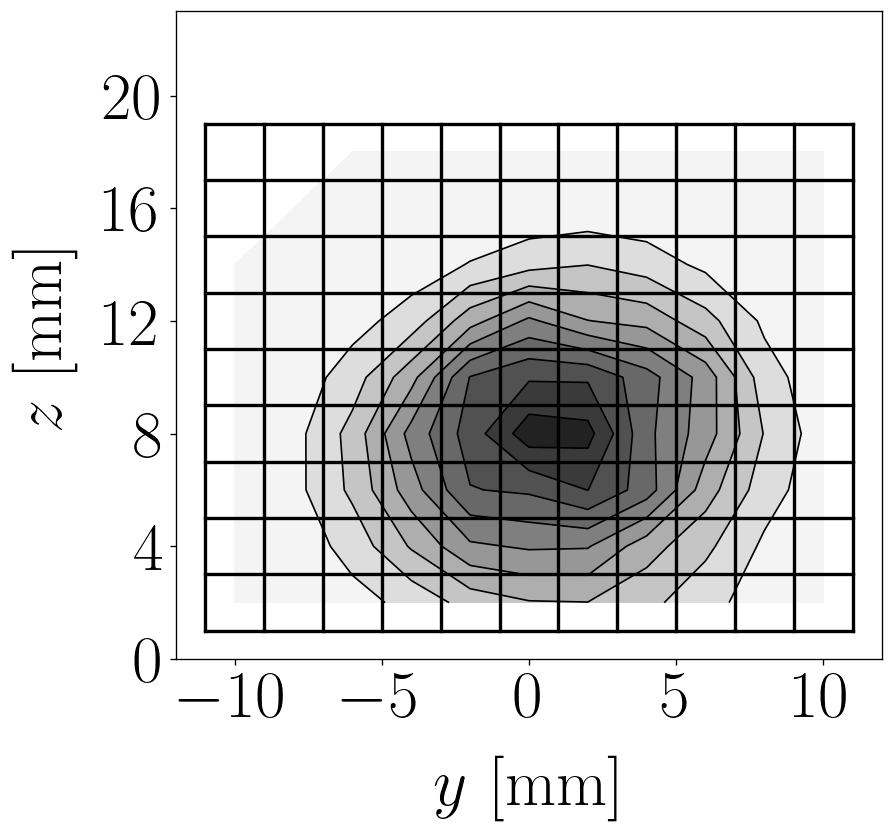
\includegraphics[scale=0.225]{./part2_developments/figures_ch6_lagrangian_JICF/previous_numerical_results/map_expe}
   \caption*{\hspace{0.35in}(a) Experimental}
   %\label{} 
\end{subfigure}
\hspace*{0.35in}
\begin{subfigure}[b]{0.2\textwidth}
	\flushleft
   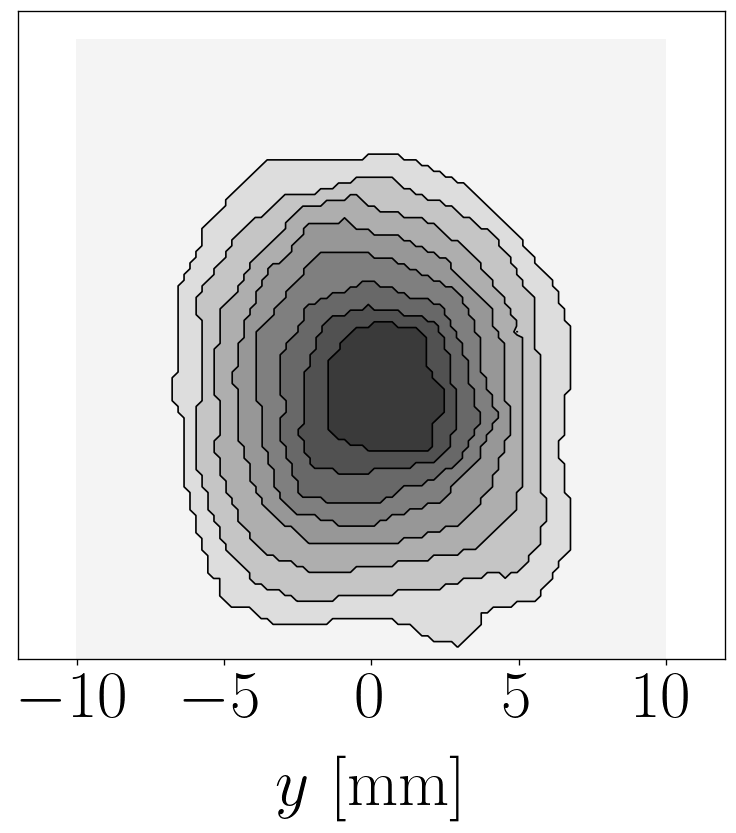
\includegraphics[scale=0.225]{./part2_developments/figures_ch6_lagrangian_JICF/previous_numerical_results/map_jaegle}
   \caption*{(b) Jaegle (2009)}
   %\label{} 
\end{subfigure}
\hspace*{0.05in}
\begin{subfigure}[b]{0.2\textwidth}
	\flushleft
   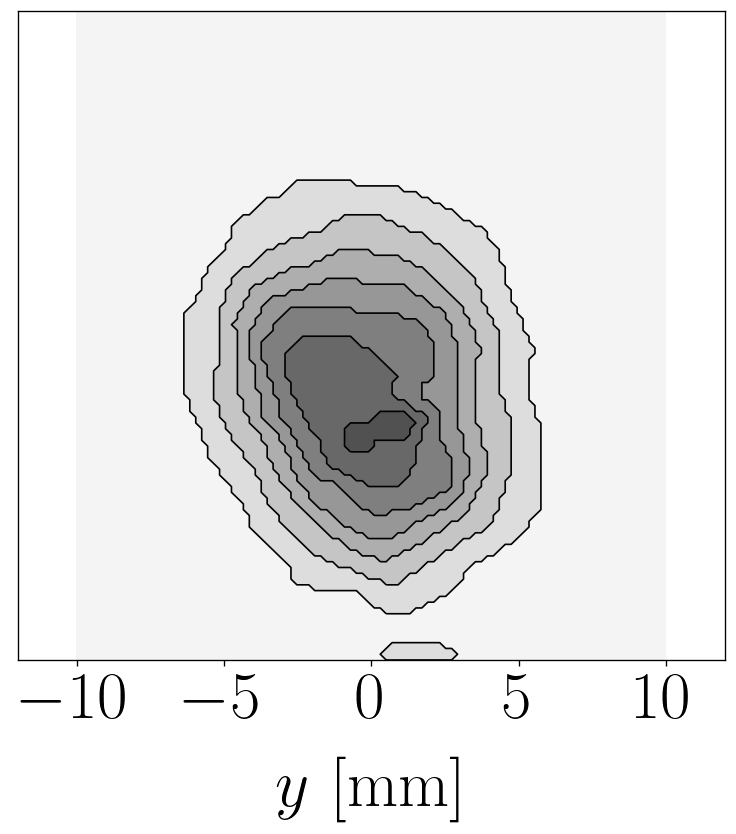
\includegraphics[scale=0.225]{./part2_developments/figures_ch6_lagrangian_JICF/previous_numerical_results/map_senoner}
   \caption*{(c) Senoner (2010)}
   %\label{} 
\end{subfigure}
\hspace*{0.05in}
\begin{subfigure}[b]{0.2\textwidth}
	\flushleft
   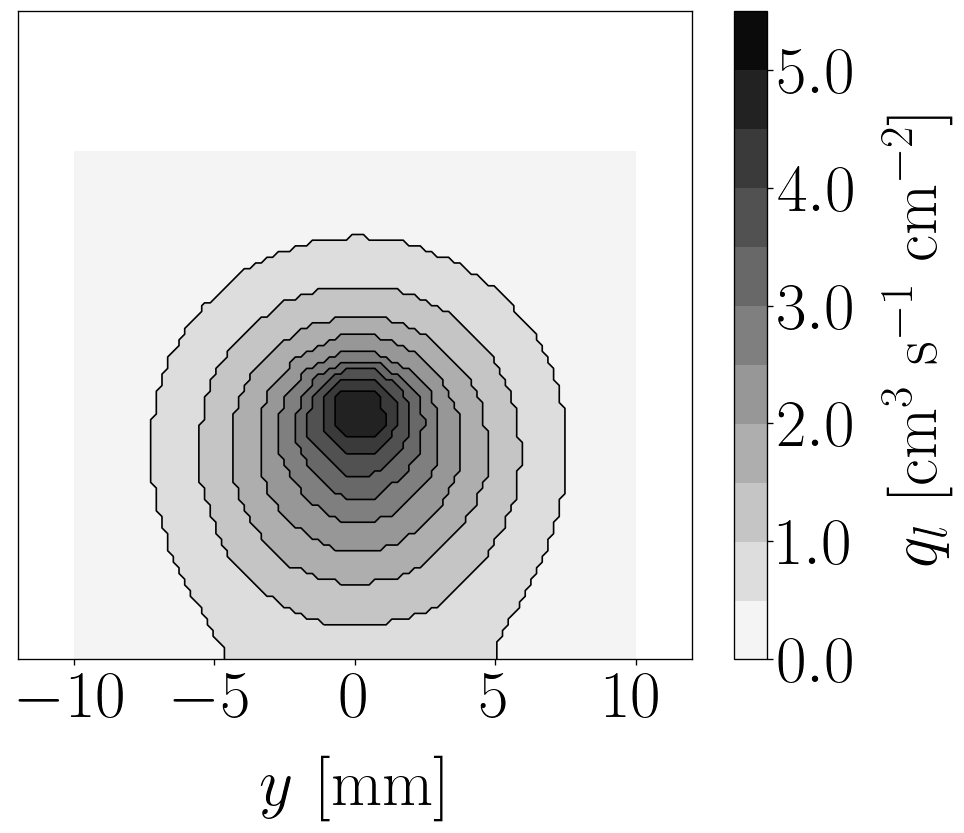
\includegraphics[scale=0.225]{./part2_developments/figures_ch6_lagrangian_JICF/previous_numerical_results/map_eckel}
   \caption*{(c) Eckel (2016)}
   %\label{} 
\end{subfigure}
\caption{Volume flux maps at $x = 80$ mm obtained for the high Weber operating conditions from experiments \citepColor[becker_breakup_2002] and past computational works on the same configuration and operating condition. The experimental map shows the grid composed of the probes through which the spray is characterized}
\label{fig:maps_previous_numerical_results}
\end{figure}

As previously mentioned, none of the previous works display SMD maps. Most of the works report, on the other hand, $SMD$ integrated profiles over $y$: these have been digitalized and are shown in Figure \ref{fig:previous_works_profiles_comparison_with_expe}.   The error bars in the experimental SMD profiles at this Figure correspond to a deviation of 10 $\%$ in each point. All cases show a ballistic behaviour in which the SMD increases with vertical distance $z$. The SMD profiles integrate over $z$ are only present in \citeColor[rachner_modelling_2002], who obtained accurate results at the center of the spray (region of maximum flux location) and showed a SMD overestimation when moving away towards the edges.

From the SMD integrated profiles over $y$, a global SMD can be estimated by performing a further integration along the $z$ direction:

\begin{equation}
 SMD =  \frac{1}{ \int_0^{L_z} \langle q_l \left( z \right) \rangle dz} \int_0^{L_z} \langle q_l \left( z \right) \rangle \langle SMD \left( z \right) \rangle dz
\end{equation}


Results are shown in Table \ref{tab:previous_numerical_studies_on_jicf_dlr_values}.  \citeColor[eckel_semi-empirical_2016] do not provide the integrated SMD profile, yet they give directly the global SMD. Generally, all SMDs show a good agreement with respect to the experimental value of \citeColor[becker_breakup_2002]. The works of \citeColor[rachner_modelling_2002] and \citeColor[eckel_semi-empirical_2016] perform a calibration of their model to match the experimental size distribution, hence such a good agreement is expected. Similar is the case of \citeColor[jaegle_large_2009], who already injected the experimental size distribution at the injector without including any secondary atomization model: then, the flux-weighted SMD is expected to be close to the SMD of this distribution. \citeColor[senoner_simulation_2010] does not inject any distribution but injects droplets at the liquid nozzle with size equal to the nozzle's diameter, drags them with a modified momentum transfer law at the column liquid region and then applies the stochastic secondary breakup model of \citeColor[gorokhovski_stochastic_2001], used in this thesis and explained in $\S$\ref{subsec:ch4_goro_model}, to account for further breakup of droplets. The good results in terms of global SMD and integrated profiles obtained in his work denote the suitabitliy of the stochastic breakup model to simulate such configurations.




%\citeColor[rachner_modelling_2002], who performed the first computations on this experimental bench, stated that the injected fuel flow rate is not conserved in the measurements at $x = 80$ mm since "\textsl{PDA measurements are less accurate at high local liquid fluxes because of dense spray effects} (sic)". \hl{...} The experimental volume flux map at $x = 80$ together with the grid in whose center the measurement probes have been located is shown in Figure \hl{\textbf{XX}} left. For each discrete probe ($j,k$), the absolute flux $Q_{l_{j,k}}$ can be calculated as:


\begin{figure}[h!]
\flushleft
\begin{subfigure}[b]{0.9\textwidth}
	\centering
   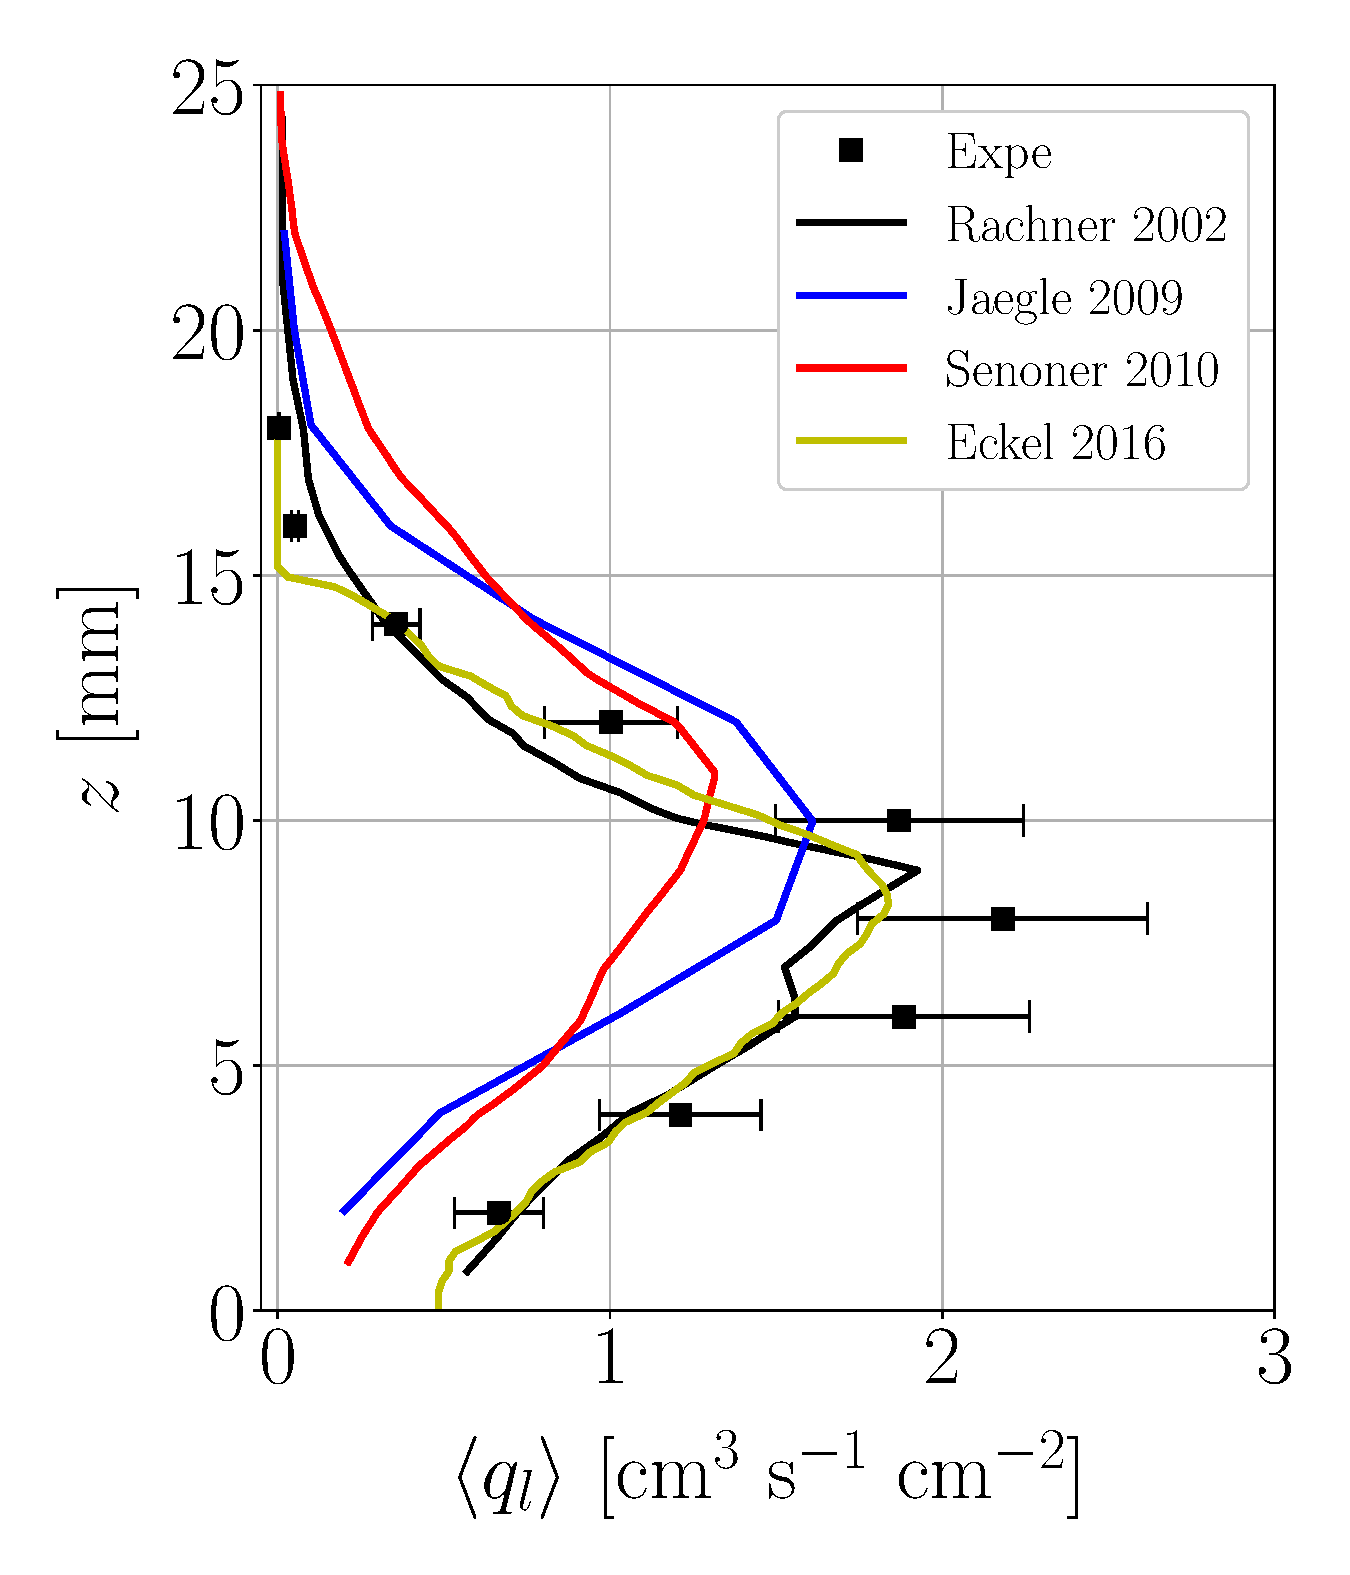
\includegraphics[scale=0.22]{./part2_developments/figures_ch6_lagrangian_JICF/previous_numerical_results/flux_profiles_along_z}
%    \hfill
   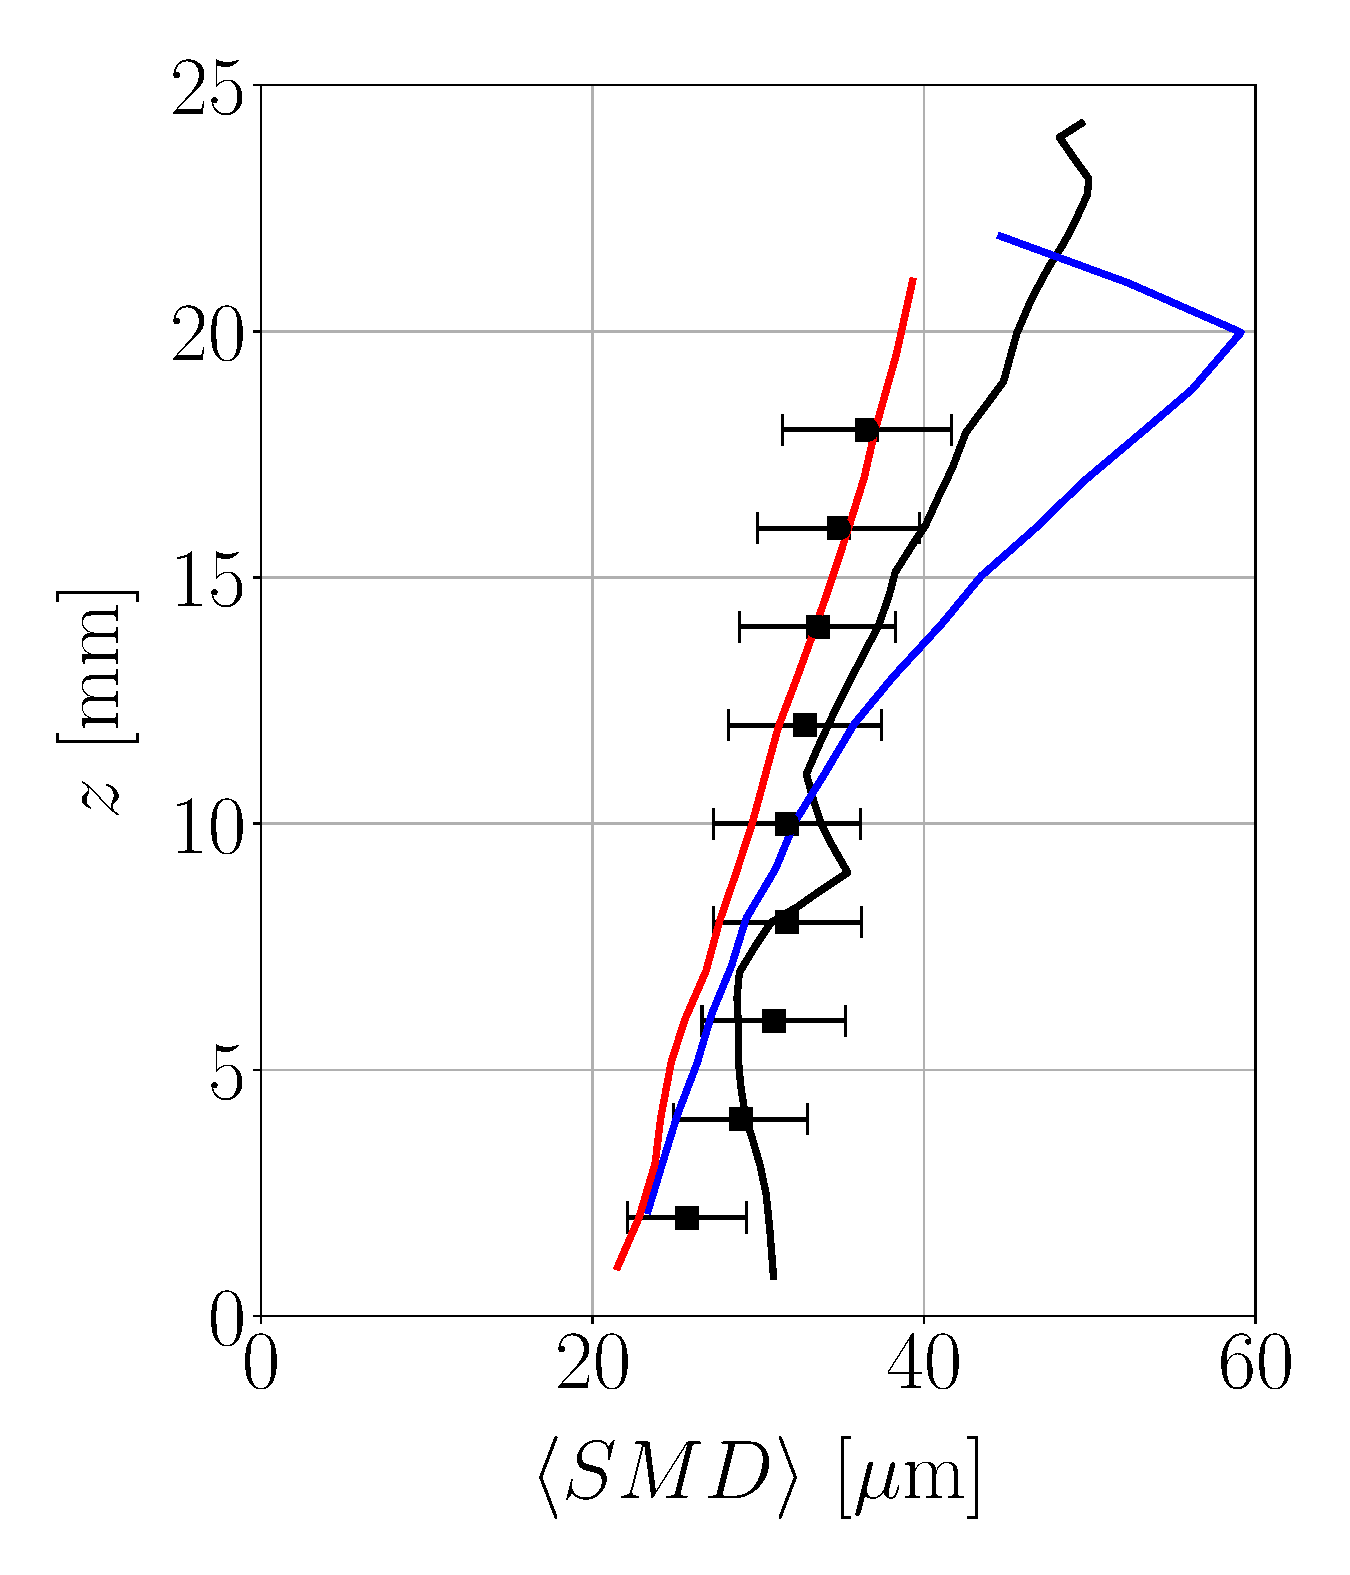
\includegraphics[scale=0.22]{./part2_developments/figures_ch6_lagrangian_JICF/previous_numerical_results/SMD_profiles_along_z}
   \caption{Profiles integrated over y}
   %\label{} 
\end{subfigure}

\vskip\baselineskip

\begin{subfigure}[b]{0.9\textwidth}
	\centering
   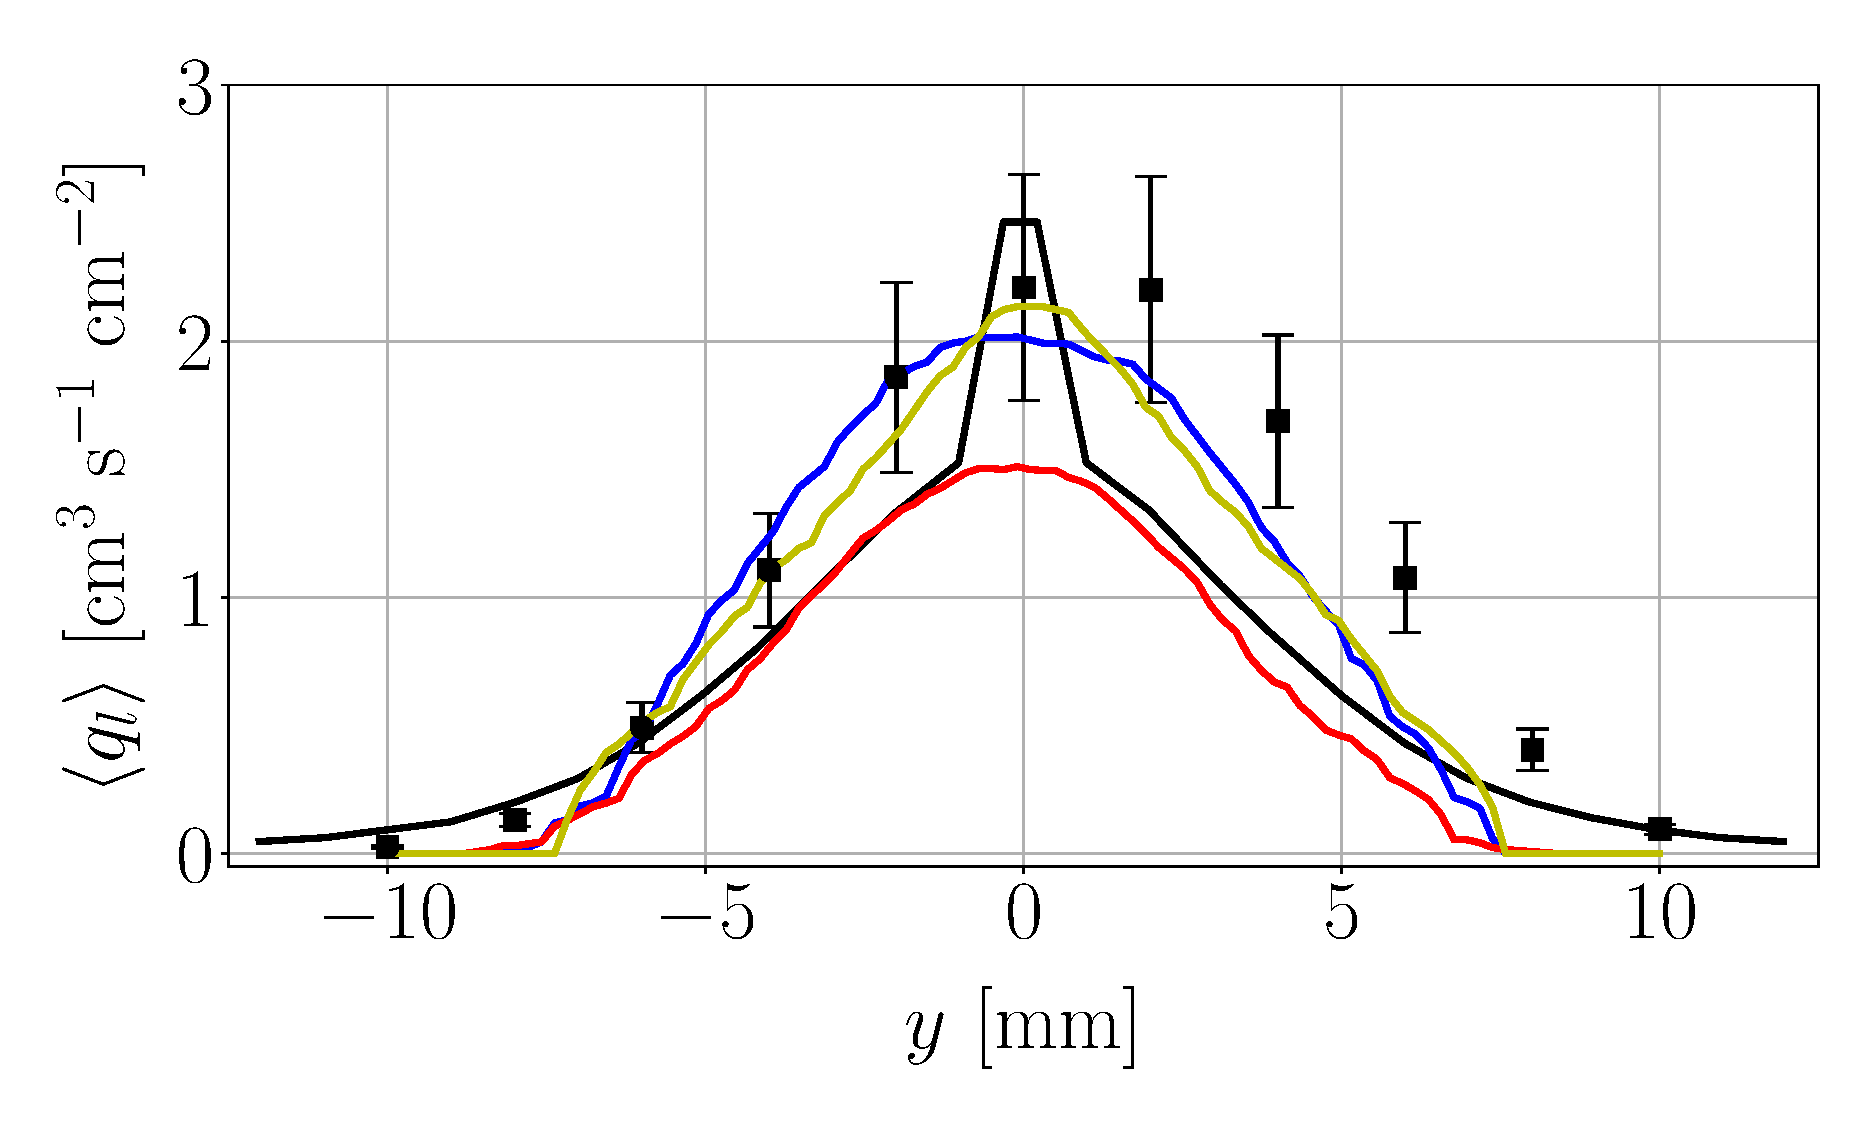
\includegraphics[scale=0.22]{./part2_developments/figures_ch6_lagrangian_JICF/previous_numerical_results/flux_profiles_along_y}
    %\hfill
   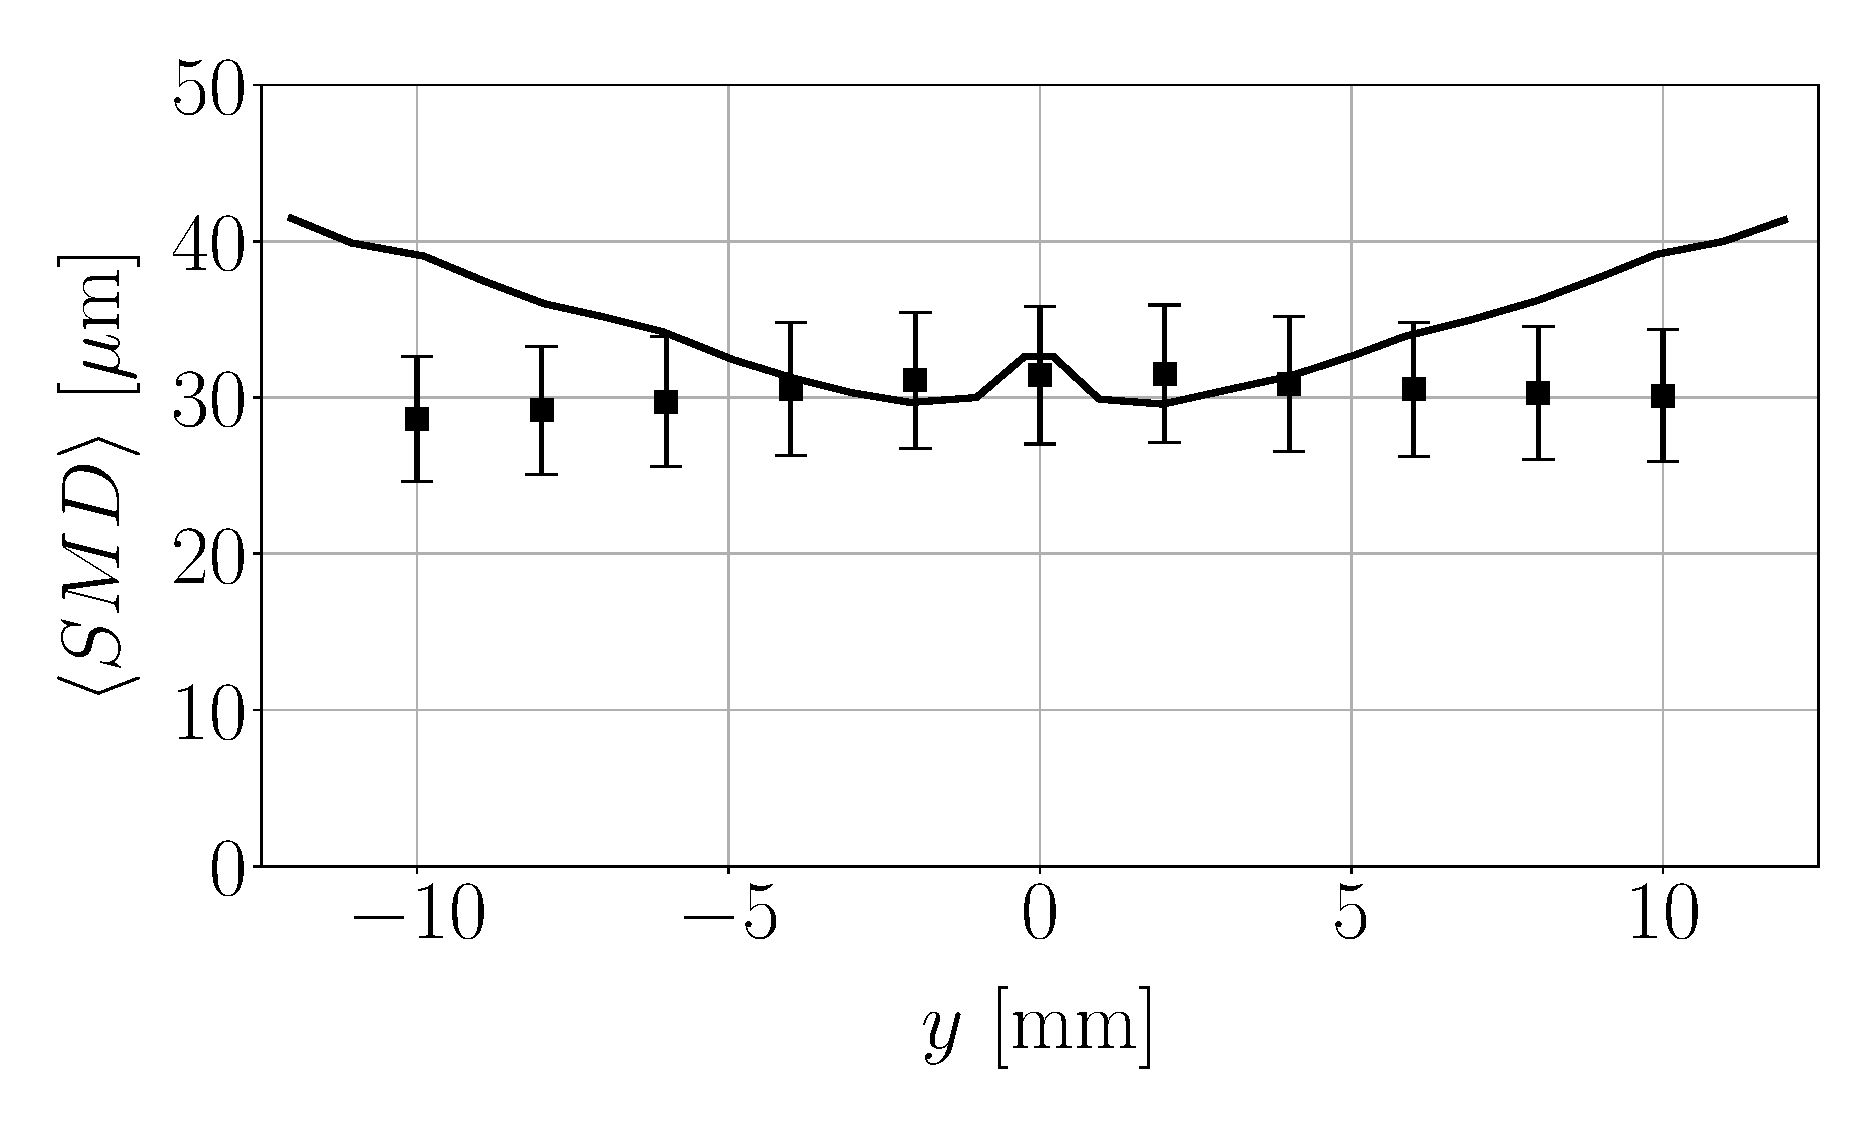
\includegraphics[scale=0.22]{./part2_developments/figures_ch6_lagrangian_JICF/previous_numerical_results/SMD_profiles_along_y}
   \caption{Profiles integrated over z}
   %\label{} 
\end{subfigure}
\caption{Integrated $SMD$ and volume flux profiles from experiments and past computational works. Computational fluxes have been obtained through digitalization and are hence not fully reliable }
\label{fig:previous_works_profiles_comparison_with_expe}
\end{figure}

\clearpage

\begin{table}[!h]
\centering
\caption{Global data obtained at $x = 80$ mm from experiments and previous computational studies }
\begin{tabular}{ccc}
\thickhline
Reference & $SMD~\left[ \mu \mathrm{m}\right]$  & $Q_l~\left[ \mathrm{mm}^3 s^{-1} \right]$ \\
\thickhline
\citeColor[becker_breakup_2002] & 31.0 &   4062  \\  
\citeColor[rachner_modelling_2002] & 31.9  & 3710  \\
\citeColor[jaegle_large_2009] & 33.2 &  3693.8  \\
\citeColor[senoner_simulation_2010] & 29.6  & 3573  \\
\citeColor[eckel_semi-empirical_2016] & 32.7  & 3775.9  \\
\thickhline
\end{tabular}
\label{tab:previous_numerical_studies_on_jicf_dlr_values}
\end{table}


%\begin{table}[!h]
%\centering
%\caption{Data obtained from previous work }
%\begin{tabular}{ccccc}
%\thickhline
%Work & $SMD~\left[ \mu \mathrm{m}\right]$ & $\varepsilon_{SMD}~\left[\% \right]$ & $Q_l~\left[ \mathrm{mm}^3 s^{-1} \right]$ & $\varepsilon_{Q_l}~\left[ \% \right]$ \\
%\thickhline
%\citeColor[becker_breakup_2002] & 31 & &  4062&  \\  
%\citeColor[rachner_modelling_2002] & 31.9 & & 3710 & \\
%\citeColor[jaegle_large_2009] & 33.2 & & 3693.8 & \\
%\citeColor[senoner_simulation_2010] & 29.6 & & 3573 & \\
%\citeColor[eckel_semi-empirical_2016] & 32. & & 3775.9 & \\
%\thickhline
%\end{tabular}
%\label{tab:previous_numerical_studies_on_jicf_dlr_values}
%\end{table}




\section{Obtention of boundary conditions for gaseous phase}
\label{sec:ch6_BC_gaseous_phase}

Prior to liquid injection, it is necessary to establish an initial solution for the gaseous phase as done for the resolved simulations. The difference with respect to the resolved simulations is that in this case, the initial solutions needs to consider the ALM since the dense core blockage effect needs to be modelled in the dispersed phase simulations. All the details of the model were addressed in $\S$\ref{sec:ch4_dense_core_modelling}. In this section, results from the resolved simulations are employed as input parameters to feed the ALM model. It is shown that the initial parameters do not capture correctly the gaseous turbulent structures, and are tuned in order to find an optimal configuration that better retrieves them. This optimal configuration is nevertheless not able to capture all the gaseous features, and another methodology to prescribe inlet boundary conditions obtained from the resolved atomization simulations in a reduced computational domain.


\subsection{Actuator Line Model}

%\subsection{Setup of actuator model}

An actuator representing the dense core can be defined for performing the dispersed-phase simulations by using results from the resolved atomization simulations as input parameters to ALM, whose control variables were summarized in Table \ref{tab:alm_parameters}. An example of an actuator representing the dense core in gaseous simulations can be seen in Figure \ref{fig:u_inst_SPS_and_ALM}. As observed, it is graphically represented as a cylinder with the initial point located in the injection nozzle exit and final point in the breakup location of the resolved dense core estimated from the resolved simulations. The actuator points (not shown in the figure) are located uniformly along the central line of the cylinder. The discrete forces applied to each point are then mollified in the neighbouring cells in order to avoid flow singularities.


\begin{figure}[h!]
	\centering	\includeinkscape[inkscapelatex=false,scale=0.6]{./part2_developments/figures_ch6_lagrangian_JICF/gas_field_initial_conditions/u_inst_SPS_and_ALM}
	\caption[Perturbation effect towards the gaseous phase visualized through the instantaneous velocity magnitude in the plane $y = 0$]{Perturbation effect towards the gaseous phase visualized through the instantaneous velocity magnitude in the plane $y = 0$. The snapshots correspond to the resolved simulation UG100\_DX10 (\textsl{left}) and to a gaseous simulation with the optimal actuator (\textsl{right})}	
	\label{fig:u_inst_SPS_and_ALM}
\end{figure}


In order to assess the ALM, the results from the high Weber operating point for the fine case (UG100\_DX10) are used: the actuator point coordinates $x_b$, $z_b$ are obtained from the mean values of Figure \ref{fig:dense_core_mean_parameters_scatterplots}, while the force $\textbf{F}_\mathrm{DC}$ is taken from Table \ref{tab:dense_core_pressures_and_force_parameters}. These values, summarized in Table \ref{tab:jicf_lgs_ALM_parameters}, represent an \textbf{initial} actuator. As it will be shown, it was found that the disturbance effect created by this actuator was not optimal to represent the disturbance effect of the dense core. Thus, the ALM control variables were tuned until finding an actuator which was found to better match the perturbed gaseous field: this one is summarized as the \textbf{optimal} actuator from Table \ref{tab:jicf_lgs_ALM_parameters}. This ALM configuration was chosen to be the optimal since it provides the best results with ALM on the dispersed-phase when compared to the experimental results on the spray ($\S$\ref{sec:SLI_LGS_gaseous_phase_effect}). Apart from this optimal actuator, two other configurations are also reported to illustrate the influence of the parameters: one in which the actuator ending point is changed to the location of the optimal configuration while keeping the force of the initial one (\textbf{ALM tilted}), and another one in which the optimal ending point is kept but the net force is increased (\textbf{ALM forced}). 


\begin{table}[!h]
\centering
\caption{Parameters of an actuator representing the dense core for the high Weber case}
\begin{tabular}{cccccc}
\thickhline
\textbf{Parameter} & \textbf{Units} &  \textbf{ALM Initial} & \textbf{ALM tilted} &  \textbf{ALM optimal} & \textbf{ALM forced} \\
\thickhline
$x_b$ & mm & 2.46 & 1.5 & 1.5 & 1.5 \\
$z_b$ & mm & 3.07 & 3.0 & 3.0 & 3.0 \\
%$c_0$ & mm & 0.45 & 0.45 \\
%$c_L$ & mm & & \\
$| \textbf{F}_\mathrm{DC} |$ & N & 0.095 & 0.095 & 0.25 & 0.30 \\
%$\Delta p$ & Pa &  & \\
\thickhline
\end{tabular}
\label{tab:jicf_lgs_ALM_parameters}
\end{table}

% Initial: L = 3.934 mm, L/2 = 1.967 mm, theta = 38.71
% Final: L = 3.354 mm, L/2 = 1.677 mm, theta = 26.565

\begin{figure}[h!]	
	\centering	\includeinkscape[inkscapelatex=false,scale=0.225]{./part2_developments/figures_ch6_lagrangian_JICF/gas_field_initial_conditions/ALM_planes_y}
	\caption{Mean axial velocity field at plane $y = 0$ for resolved case UG100\_DX10 and the three actuators tested. The grey cylinder represents the actuator, i.e. the location where body forces are applied}
	%\caption{Mean axial velocity field at plane $y = 0$ for resolved case UG100\_DX10 (\textsl{top left}), gaseous solutions without dense core perturbation (\textsl{top right}), with initial ALM (\textsl{bottom left}) and with optimal ALM (\textsl{bottom right})}
	\label{fig:ALM_gas_fields_plane_Y}
\end{figure}


In first place, the mean axial velocity fields in the symmetry plane $y = 0$ are shown in Figure \ref{fig:ALM_gas_fields_plane_Y}. The resolved case UG100\_DX10 is also displayed for comparison.  As observed, the initial actuator model creates only a slight perturbation downstream the cylinder location, but cannot properly retrieve the recirculation and deceleration regions which were captured by the resolved simulation. By changing only the actuator coordinates (tilted configuration), the perturbation effect is intensified and more distributed in space, since the angle $\theta$ increases and the imposed drag force is increased while the lift is reduced (Eqs. (\ref{eq:ALM_SLI_lift_drag_definitions})). This increase of the axial perturbation with changing coordinates is also reflected in the profiles of Figures \ref{fig:JICF_ICS_ALM_lines_y0_along_z_ux_mean} and \ref{fig:ALM_gas_fields_plane_x}, which show the mean axial velocity along the lines plotted in Figure \ref{fig:ALM_gas_fields_plane_Y}: the tilted profile shows a slighly larger deviation when compared to the initial one, even though its perturbation is not yet close to the resolved profile. Indeed, the lift force imposed is not large enough and the streamlines do not deviate towards the vertical direction as in the resolved case, staying oriented towards the crossflow direction as in the unperturbed case. If the force is increased (optimal configuration), the velocity field from Figure \ref{fig:ALM_gas_fields_plane_Y} shows a noticeable decrease in the axial velocity downstream the ALM region, with an increase also in the lift force as in this case streamlines are deviated upwards. The velocity profiles from Figures \ref{fig:JICF_ICS_ALM_lines_y0_along_z_ux_mean} and \ref{fig:ALM_gas_fields_plane_x} show this greater perturbation when compared to the previous cases. Nevertheless, the disturbance is still not strong enough to capture the recirculation bubble which is observed in the resolved simulation. A further increase in the net force imposed (forced configuration) shows effectively a larger perturbation which can actually capture a recirculation bubble behind the ALM region, even its location is shifted upwards with respect to the bubble from the resolved case. The profiles from Figures \ref{fig:JICF_ICS_ALM_lines_y0_along_z_ux_mean} and \ref{fig:ALM_gas_fields_plane_x} reflect this larger perturbation through the velocity profiles. However, even if the force configuration case seems to better the resolved perturbed field since it recovers the recirculation bubble, its stronger perturbation was found to greatly affect secondary atomization of the droplets in dispersed-phase simulations, yielding smaller droplets. Therefore, the reported optimal configuration is chosen as the actual optimal since it produced the best spray results among all the ALM cases. Forces in between the ones corresponding to the optimal and forced configurations were also tested (not reported here), without improving the dispersed-phase results with respect to the optimal one.





\begin{figure}[ht]
\flushleft
\begin{subfigure}[b]{0.45\textwidth}
	\centering
   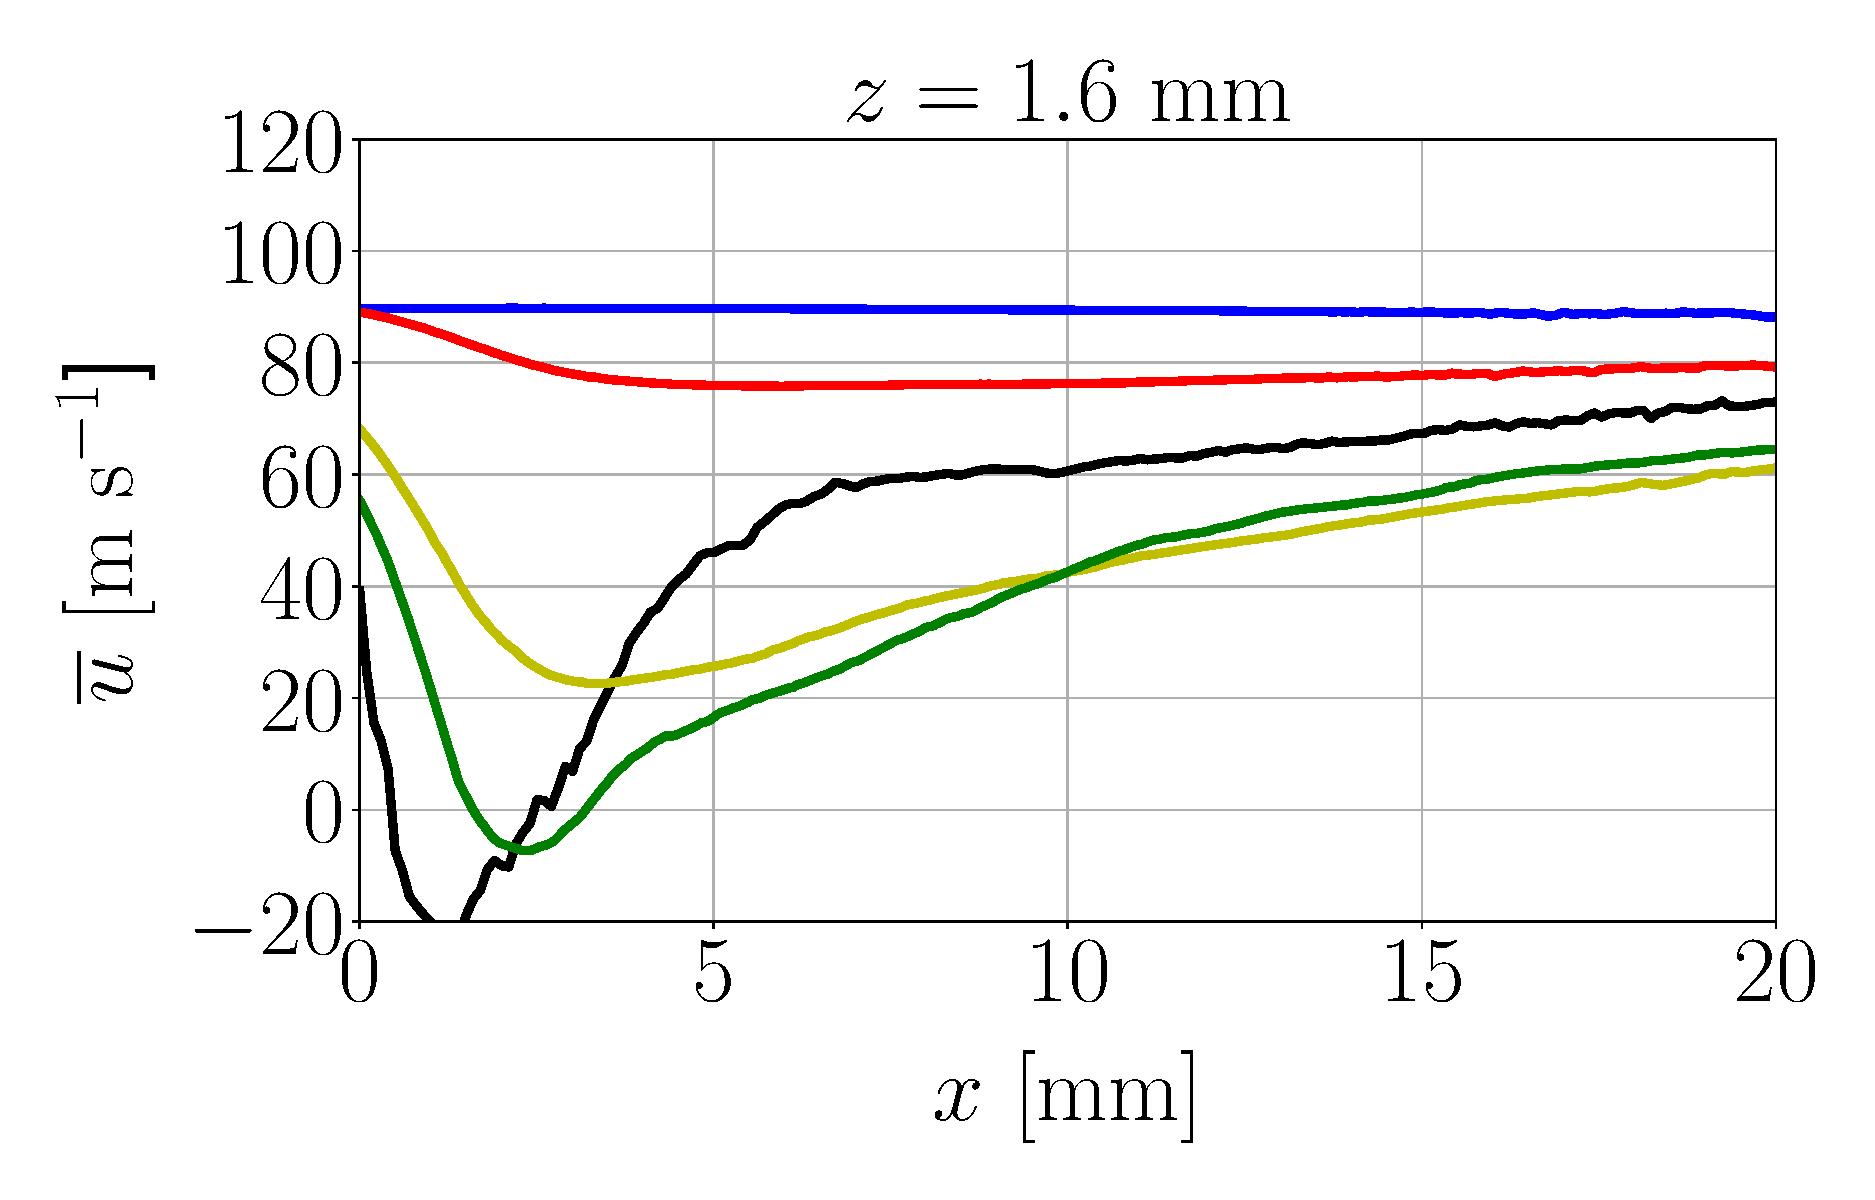
\includegraphics[scale=0.25]{./part2_developments/figures_ch6_lagrangian_JICF/gas_field_initial_conditions/ALM_line_y0_along_x_z01p6}
   %\caption{}
   %\label{} 
\end{subfigure}
\hspace{0.4in}
\begin{subfigure}[b]{0.45\textwidth}
	\centering
   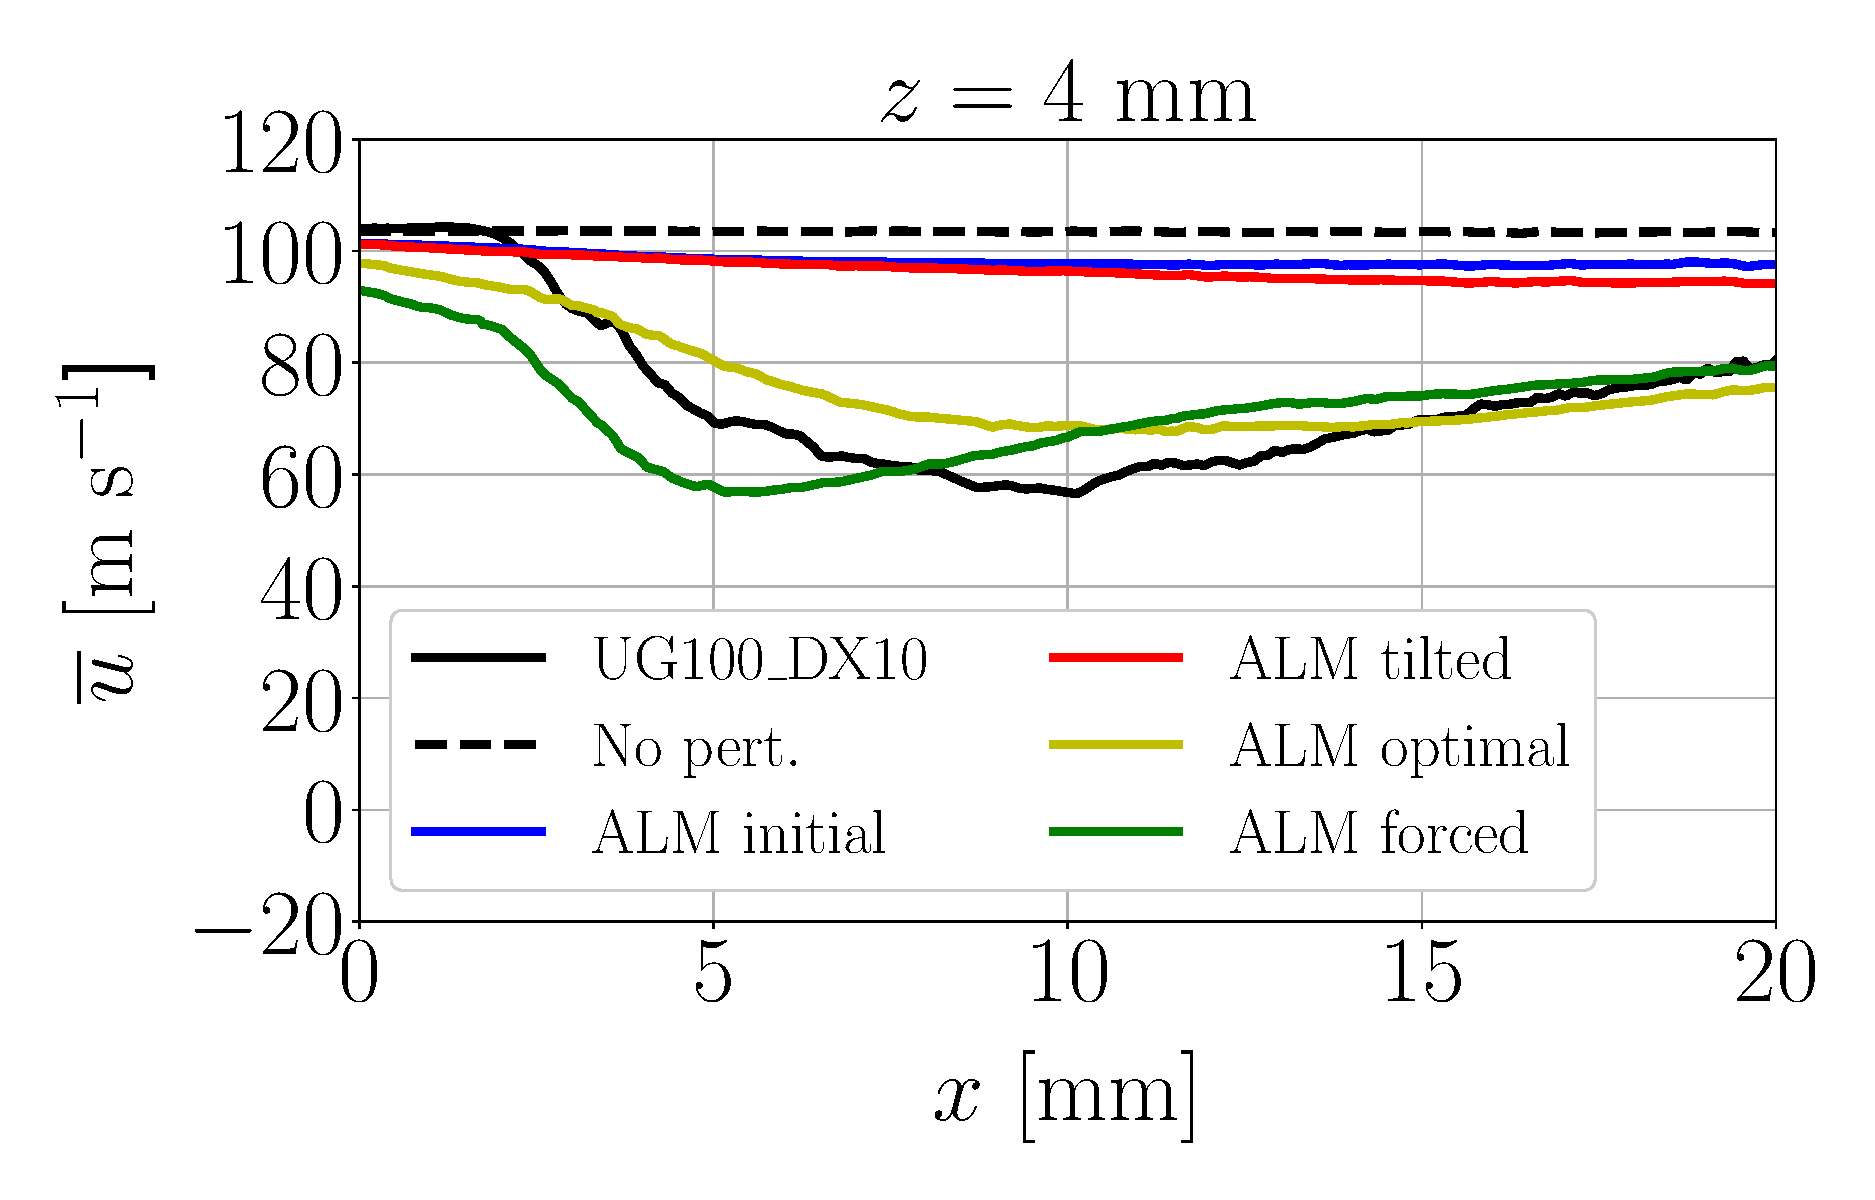
\includegraphics[scale=0.25]{./part2_developments/figures_ch6_lagrangian_JICF/gas_field_initial_conditions/ALM_line_y0_along_x_z04p0}
   %\caption{}
   %\label{}
\end{subfigure}
\caption{Mean axial velocity evolution in ALM and resolved simulations along axial coordinate at locations $z = 1.6, 4$ mm in plane $y = 0$ (lines of Figure \ref{fig:ALM_gas_fields_plane_Y})}
\label{fig:JICF_ICS_ALM_lines_y0_along_x_ux_mean}
\end{figure}

\begin{figure}[ht]
\centering
   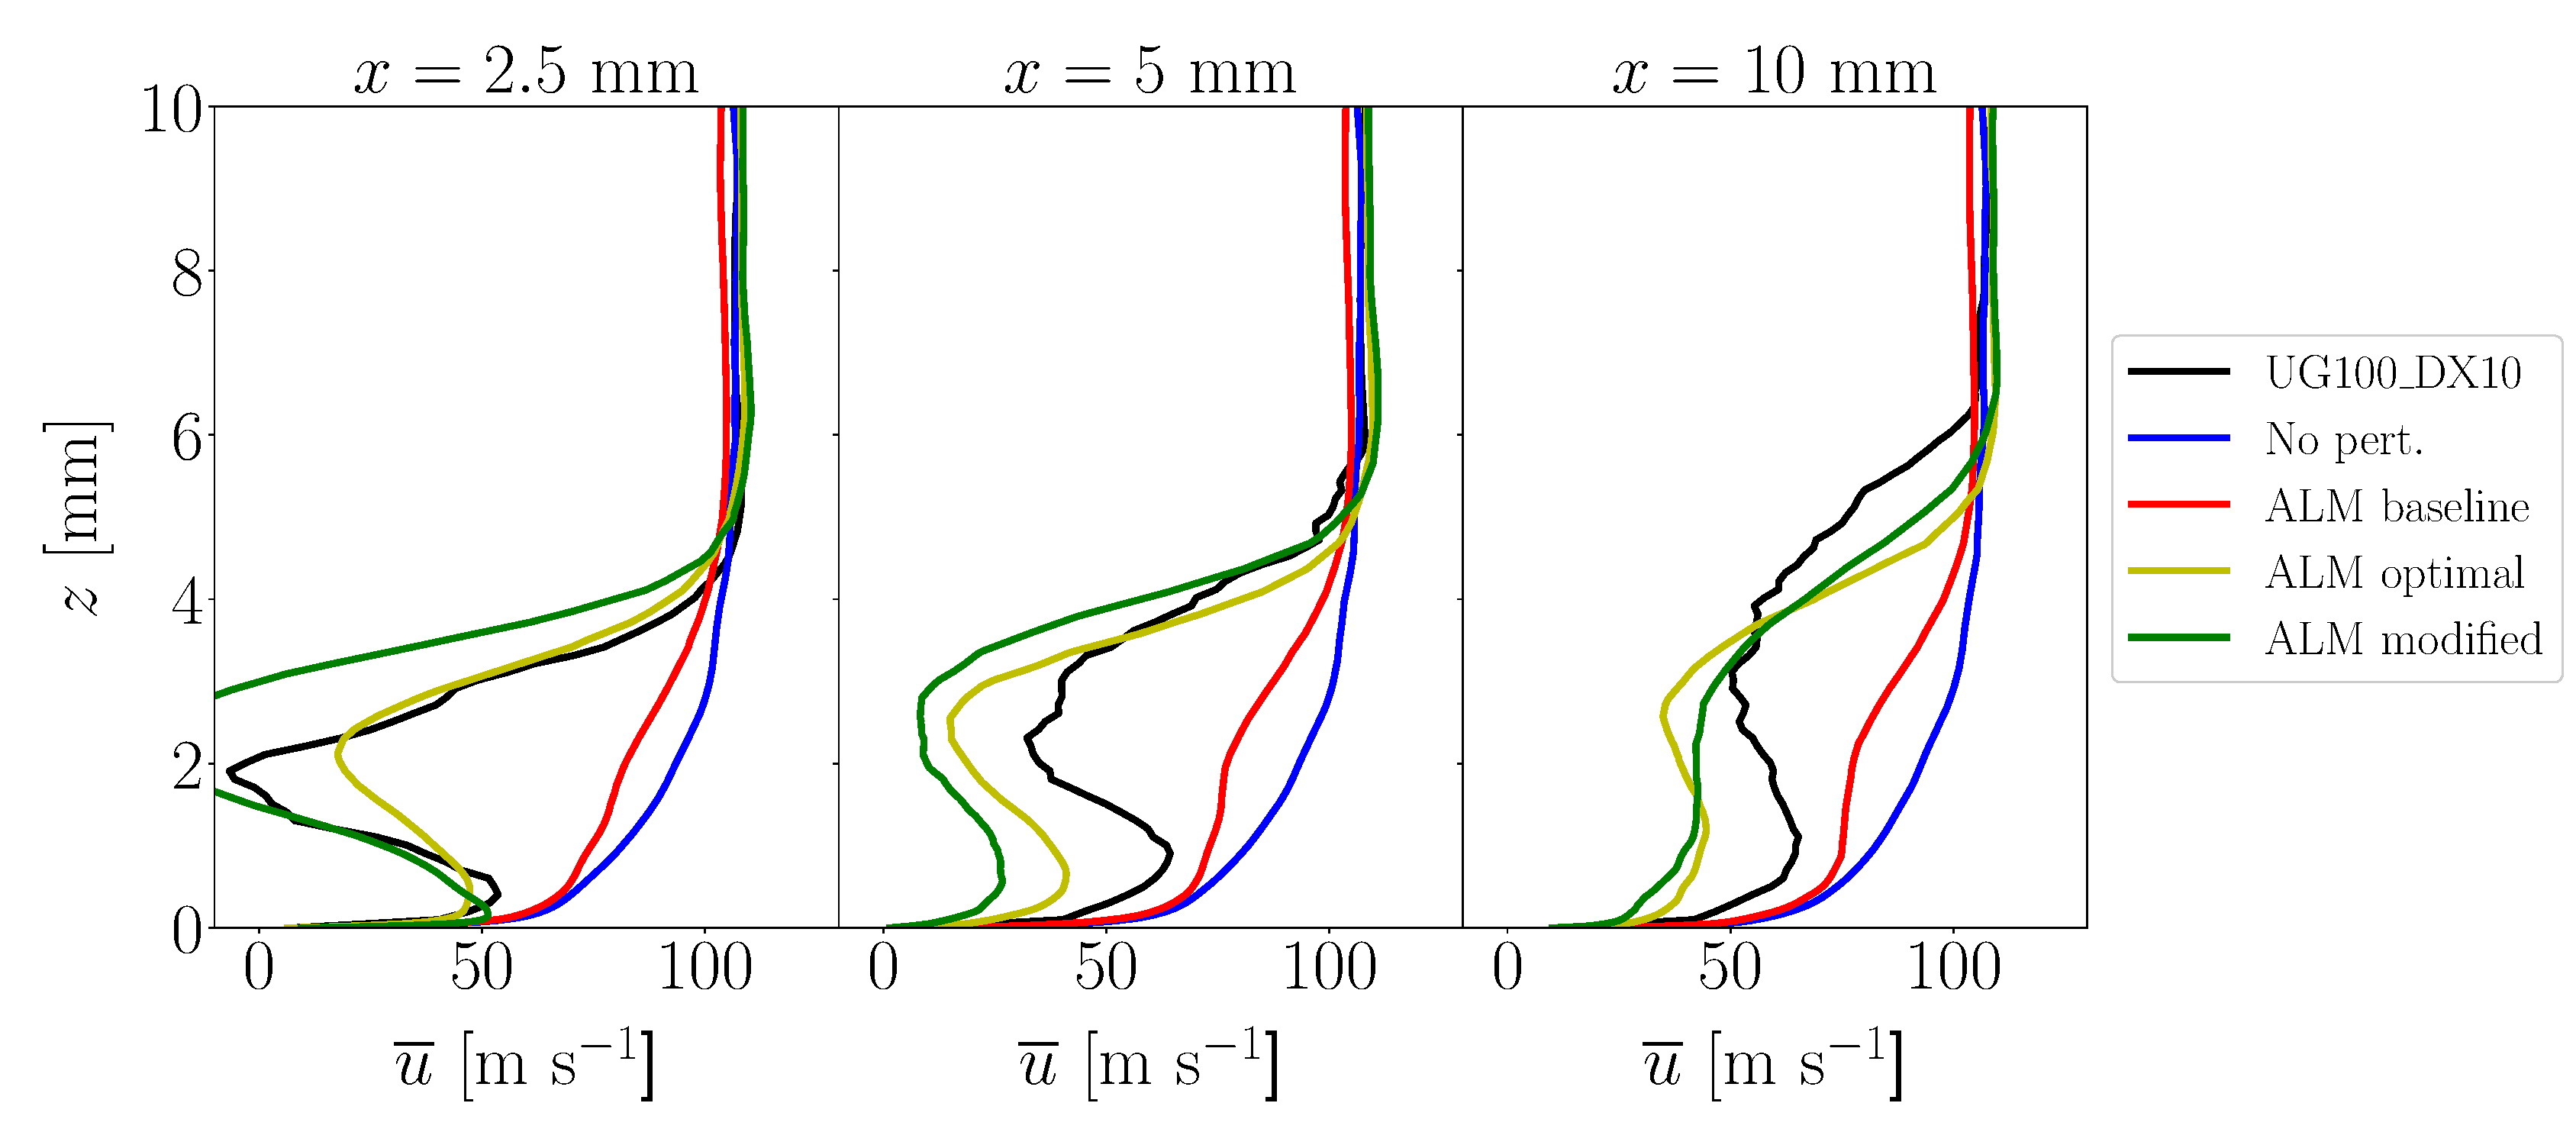
\includegraphics[scale=0.26]{./part2_developments/figures_ch6_lagrangian_JICF/gas_field_initial_conditions/ALM_lines_y0_along_z_ux_mean}
\caption{Mean axial velocity evolution in ALM and resolved simulations along vertical coordinate at $x = 2.5, 5, 10$ mm locations of plane $y = 0$ (lines of Figure \ref{fig:ALM_gas_fields_plane_Y})}
\label{fig:JICF_ICS_ALM_lines_y0_along_z_ux_mean}
\end{figure}

Since the purpose of ALM is trying to capture the gaseous perturbations of the dense core as close as possible, it is also of interest to look at the planes perpendicular to the crossflow. Figure \ref{fig:ALM_gas_fields_plane_x} shows the mean velocity fields at planes $x = 5, 10$ mm compared to the resolved cases. In the same was as in plane $y = 0$, modifying the actuator ending coordinates and increasing the net dense core reduced further the mean velocities in the flow field. This has also a strong effect in the counter-rotating vortices (CRVs) of the flow, which are an important characteristic of the JICF that can affect the transport and atomization of the droplets. Cases unperturbed and ALM initial do not show CRVs in the flow as shown by the flow streamlines, while the ALM tilted and optimal cases can retrieve quite accurately the location,  intensity and rotation direction of the resolved vortices. Further increasing the net force shows still vortical structures, yet these are small and differ from the shape of the resolved ones. In fact, a further increase in the force (not reported here) was also checked and showed that the CRVs inverted their rotation direction, which is an unphysical behaviour in the JICF \citepColor[karagozian_analytical_1986].


\begin{figure}[h!]	
	\centering	\includeinkscape[inkscapelatex=false,scale=0.20]{./part2_developments/figures_ch6_lagrangian_JICF/gas_field_initial_conditions/ALM_planes_x}
	\caption{Mean axial velocity field at planes $x = 5, 10$ mm for resolved case UG100\_DX10 and gaseous cases with and without ALM}
	\label{fig:ALM_gas_fields_plane_x}
\end{figure}

Finally, the velocity profiles along the white lines from Figure \ref{fig:ALM_gas_fields_plane_x} are plotted in Figure \ref{fig:JICF_ALM_lines_iso-x_along_y_ux_mean}. Again, the initial and tilted ALM do not create a noticeable disturbance in the flow field compared to the resolved case, except at $z = 1.6$ mm in plane $x = 10$ mm where the tilted case shows the closest match of all models. Increasing the force approaches the resolved perturbation at plane $x = 5$ mm: the optimal ALM shows a good match at $z = 1.6$ mm, while the equivalent occurs for the force ALM further away from the wall at $z = 5$ mm. For the profiles at $z = 5$ mm in plane $x = 10$ mm, none of the actuators could achieve the intensity of the resolved perturbation: ALM creates the greatest perturbations downstream the actuator region but has a very limited influence further vertically from its ending point, which is not the case of a resolved dense core since the ligaments created during primary atomization also create perturbations in the gas field away from the dense core. 

\begin{figure}[ht]
\centering
\begin{subfigure}[b]{1.0\textwidth}
	\centering
   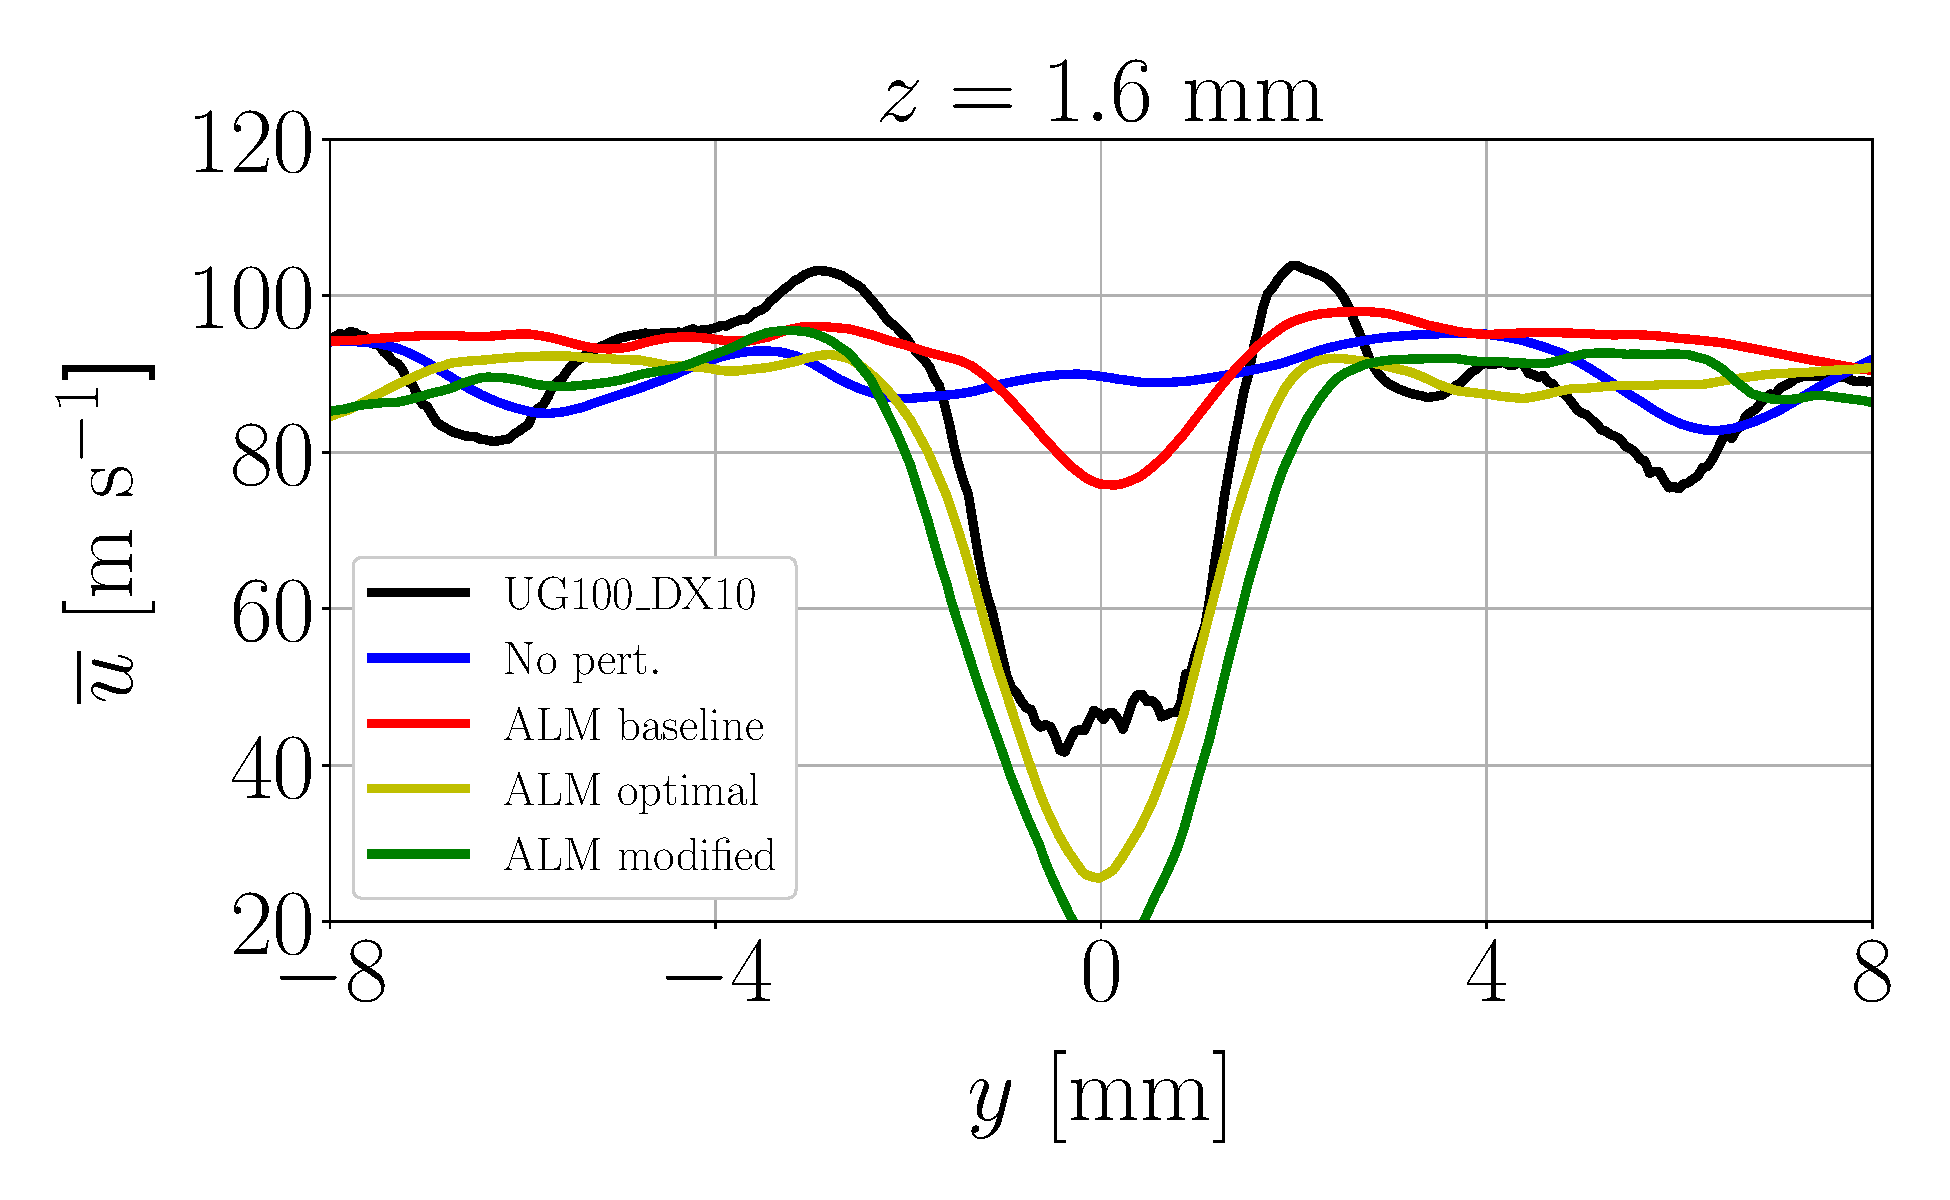
\includegraphics[scale=0.24]{./part2_developments/figures_ch6_lagrangian_JICF/gas_field_initial_conditions/ALM_line_x05_z01p6_ux_mean_along_y}
   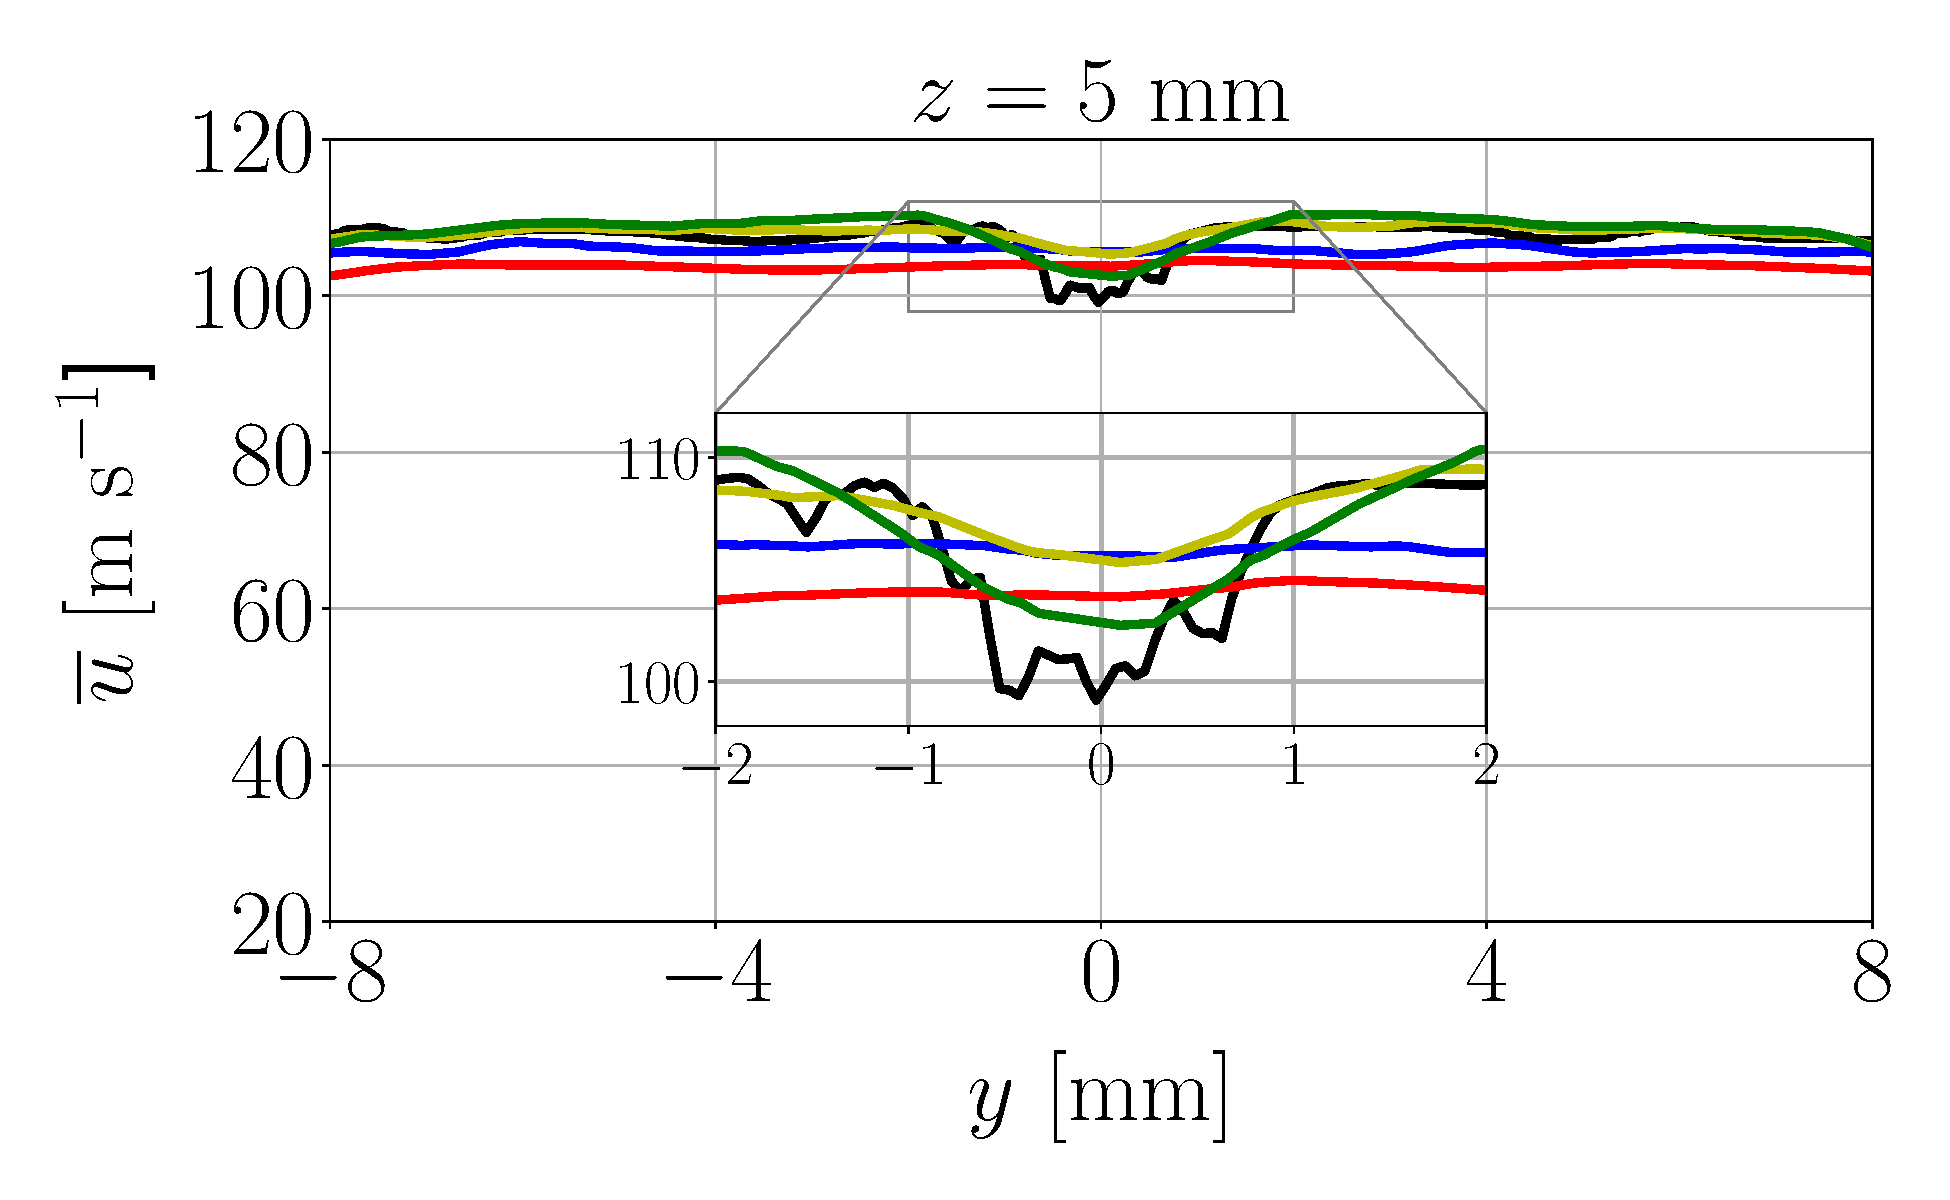
\includegraphics[scale=0.24]{./part2_developments/figures_ch6_lagrangian_JICF/gas_field_initial_conditions/ALM_line_x05_z05p0_ux_mean_along_y}
   \vspace*{-0.1in}
	\caption{Plane $x = 5$ mm}
\end{subfigure}
\vskip\baselineskip
\begin{subfigure}[b]{1.0\textwidth}
	\centering
   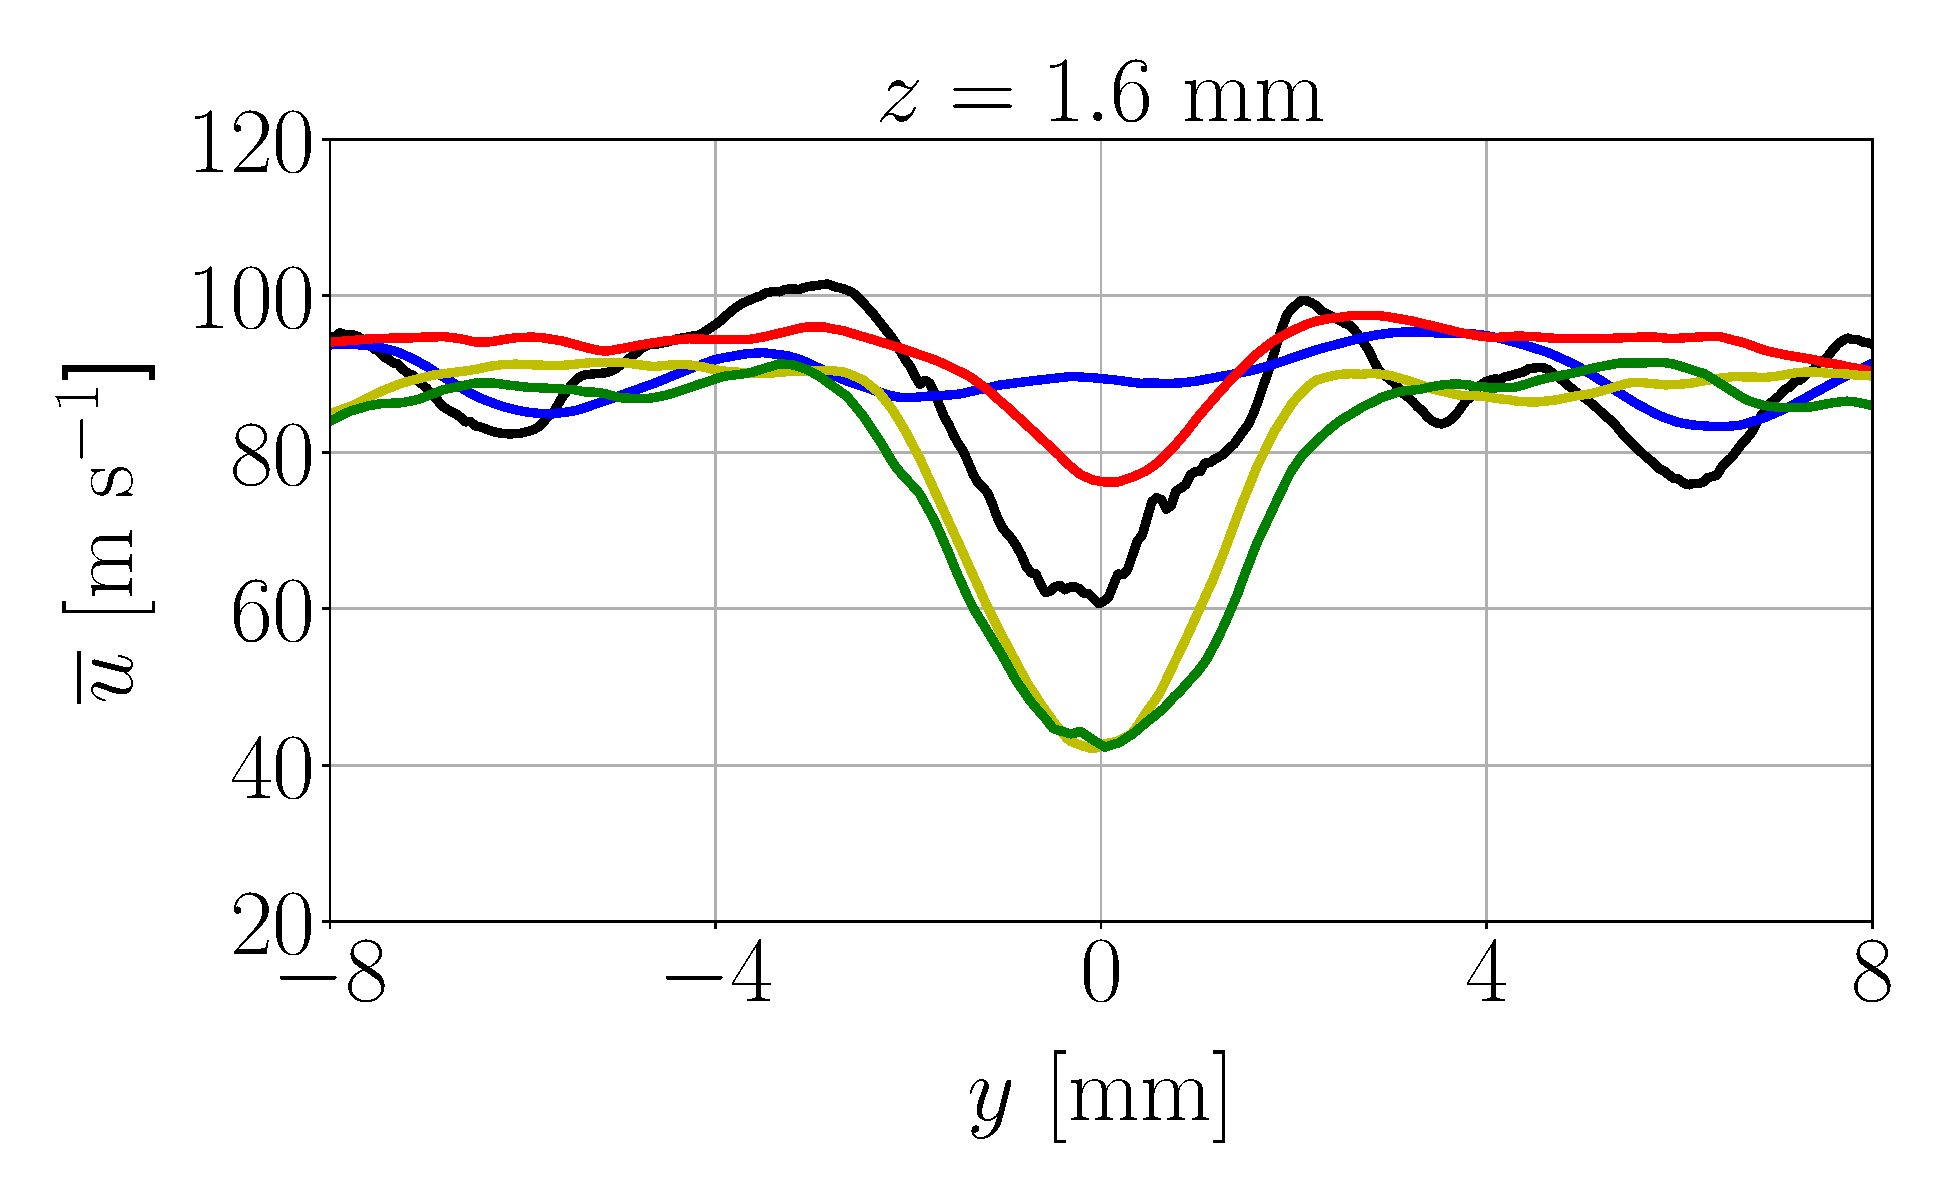
\includegraphics[scale=0.24]{./part2_developments/figures_ch6_lagrangian_JICF/gas_field_initial_conditions/ALM_line_x10_z01p6_ux_mean_along_y}
   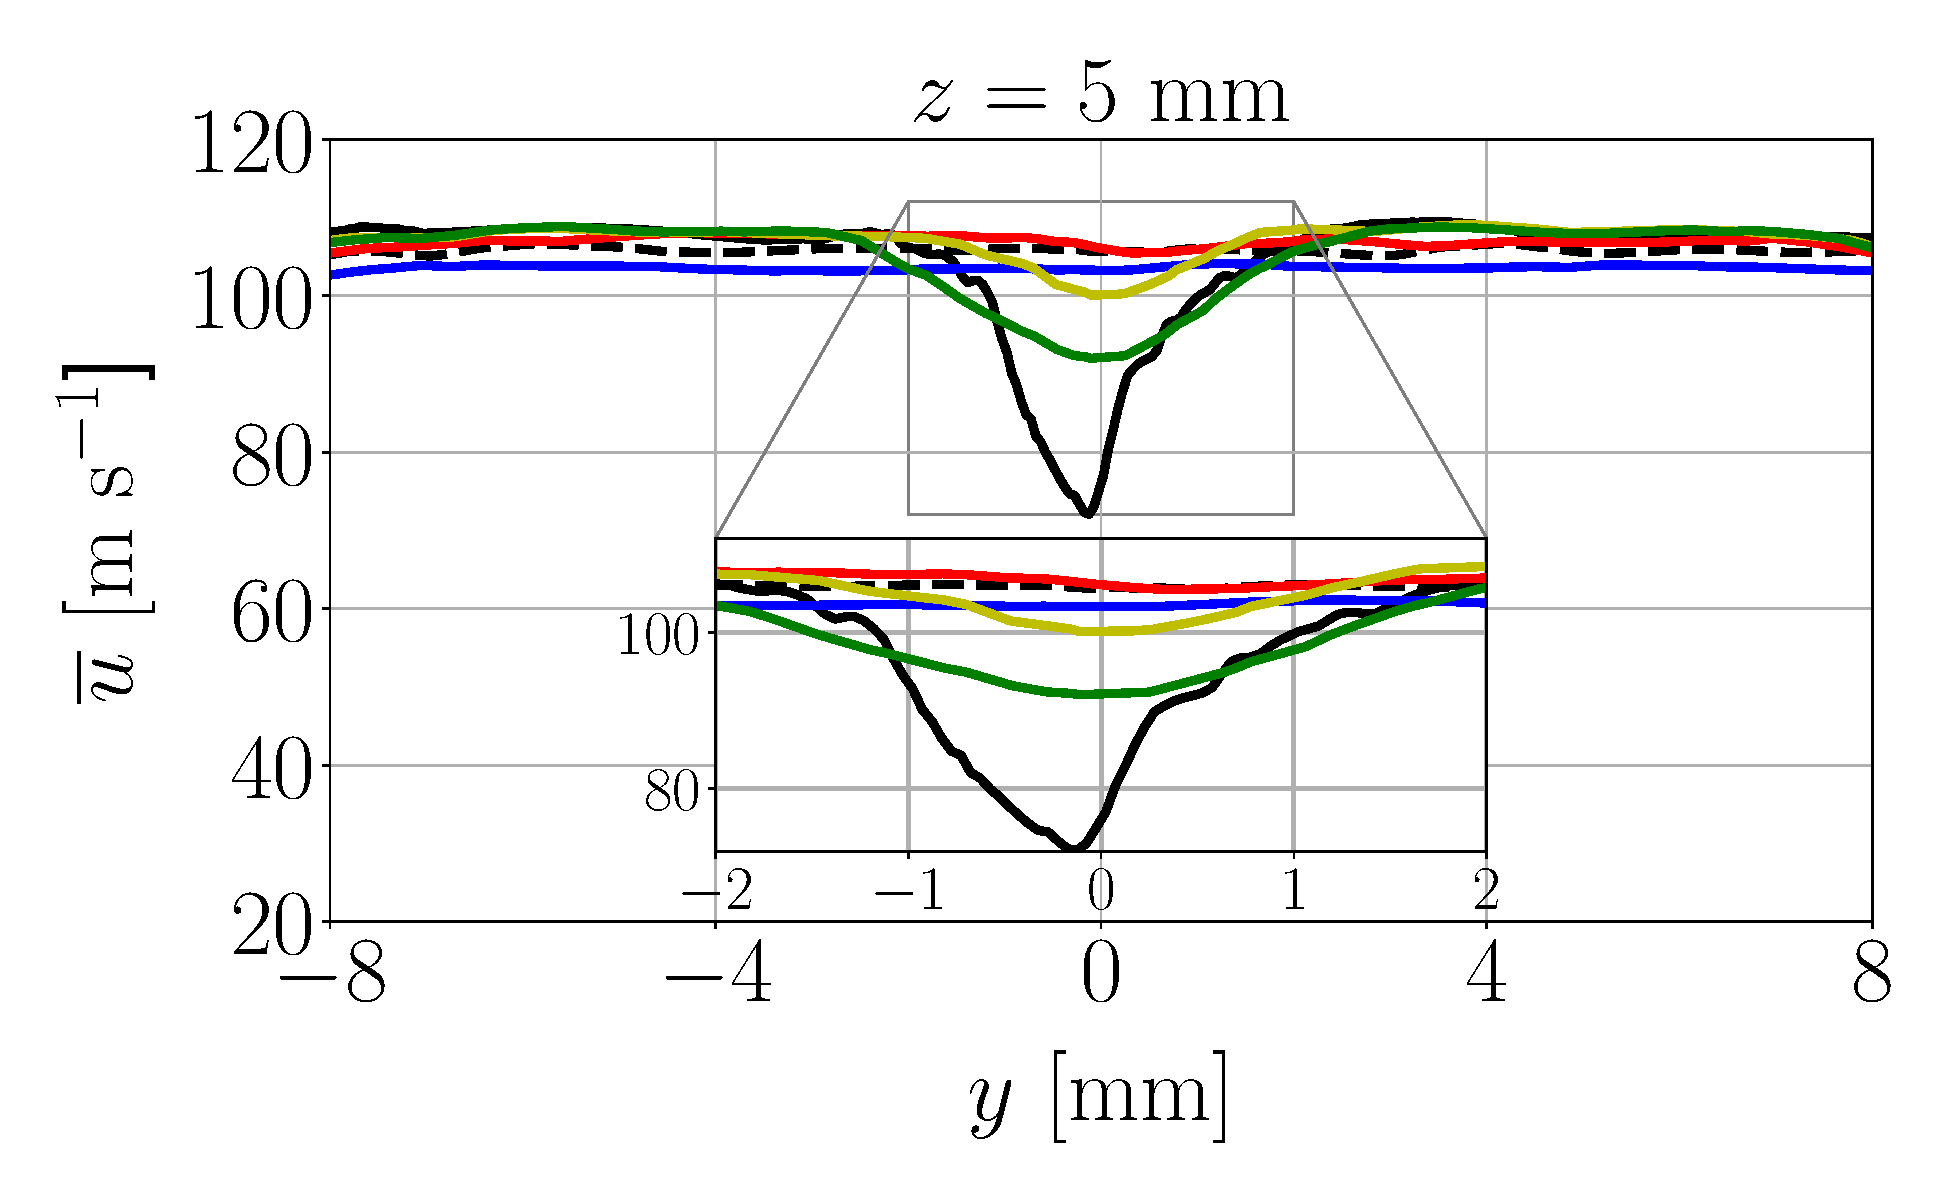
\includegraphics[scale=0.24]{./part2_developments/figures_ch6_lagrangian_JICF/gas_field_initial_conditions/ALM_line_x10_z05p0_ux_mean_along_y}
   \vspace*{-0.1in}
	\caption{Plane $x = 10$ mm}
\end{subfigure}
   \caption{Mean axial velocity evolution along lateral coordinate in ALM and resolved simulations at $z$ lines of Figure \ref{fig:ALM_gas_fields_plane_x}}
\label{fig:JICF_ALM_lines_iso-x_along_y_ux_mean}
\end{figure}

In general, it can be concluded that ALM can  perturb the gaseous field through the application of body forces but with a limited influence due to its simplified geometry, which cannot properly retrieve the complex topology of the dense core. The actuator model parameters have been tuned by a trial-and-error process to find an optimal configuration based on the ALM effect in the sprays fields, which are later analyzed in $\S$\ref{sec:SLI_LGS_gaseous_phase_effect}. A better methodology to find optimal configuration for ALM would be through a multivariable optimization process which explores the ALM parameters to better represent the resolved gaseous field through the minimization of an objective function. Furthermore, improvements in the model could also include modifications in the ALM geometry such as the inclusion of several actuator models, of the inclusion of frequential effects which can better represent the dense core unsteady shape. Such strategies were out of the scope of this thesis and are left for future work. 


\subsection{Prescription of gaseous inlet from resolved simulations }
\label{subsec:ch6_jicf_lgs_gaseous_inlet_prescription}



%\subsubsection*{Methodology}


As previously shown, the ALM model has been proved to be able to perturb the gaseous field. From an initial actuator obtained with input parameters from the resolved atomization simulation, the ALM variables have been tuned to seek for a better match of the mean velocity profiles. This match, however, is not totally accurate and the perturbation effect from the resolved simulations cannot be fully captured with ALM, since the dynamics and topology of the liquid dense core cannot be properly represented with the proposed actuator parameters. 

With the objective of trying to improve the matching of the resolvded gaseous fields, an alternative to ALM is proposed in this section. This one is based on obtaining the gaseous field in a plane perpendicular to the crossflow from the resolved simulations. The field is characterized by the mean and RMS values of the velocities in the three directions. Such profiles are then imposed in a reduced domain consisting of a box with length $150$ mm and cross-section 25x40 mm$^2$ representing the downstream part of the plenum from the JICF configuration of Figure \ref{fig:numerical_setup_maquette_JICF_DLR}. A schematic of the methodology is illustrated in Figure \ref{fig:custom_inlet_methodology}. The velocity profiles are imposed at the inlet of the prescribed domain according to the following law:

\begin{equation}
\label{eq:prescribed_inlet_u_gas_injection_law}
\textbf{u} \left( \textbf{x}, t \right) = \overline{\textbf{u}} \left( \textbf{x} \right)  + r \left( t \right)  \textbf{u}_\mathrm{RMS} \left( \textbf{x} \right) 
\end{equation}

where $\overline{\textbf{u}} \left( \textbf{x} \right)$ and $\textbf{u}_\mathrm{RMS} \left( \textbf{x} \right)$ are the mean and RMS velocity distributions in the crossflow plane extracted from the resolved atomization simulations. $r \left( t \right)$ is a time-varying scalar sampled from a normal distribution with mean 0 and variance 1: $r \sim \mathcal{N} \left( \mu = 0, \sigma^2 = 1 \right)$. This velocity prescription law, which is based on the weak recycling method of synthetic turbulence injection by \citeColor[wu_large_1995], ensures that the injected $TKE$ in the dispersed phase simulations is the same as the one retrieved from the resolved atomization ones. %\hl{Nevertheless, due to the coarser mesh employed in the reduced domain with respect to the }

\begin{figure}[h!]	
	\centering	\includeinkscape[inkscapelatex=false,scale=0.25]{./part2_developments/figures_ch6_lagrangian_JICF/gas_field_initial_conditions/custom_inlet_methodology}
	\caption{Methodology to prescribe mean and RMS velocity fields from resolved simulations in reduced domain for dispersed-phase computation.}
	\label{fig:custom_inlet_methodology}
\end{figure}

The mesh employed for performing simulations with the prescribed inlet is shown in Figure \ref{fig:mesh_reduced_inlet}. The mesh, which contains $12 \cdot 10^6$ elements, has been refined up to a location $x = 40$ mm downstream the inlet to a mesh size $\Delta x = 0.3$ mm, while from $x = 40$ mm up to $x = 100$ mm, the mesh size has been set to $\Delta x = 0.5$ mm as in the mesh of Figure \ref{fig:jicf_dlr_mesh_LGS}. The finer cell size of $\Delta x = 0.3$ mm has been selected  with the objective of better capturing the turbulent structures created by the inhomogeneous gaseous velocity profile injected. Nevertheless, this cell size is not resolved enough to capture those: in the resolved simulations of Chapter \ref{ch5:jicf_resolved_simulations}, the cell size in the gaseous field around the liquid regions was of the order of the interface cell sizes ($20, 10~\mu$m) created by the ALM method, while such resolutions cannot be imposed into this reduced domain as the mesh size greatly increases and yields computations considerably expensive. Furthermore, a too fine mesh would create large volume fractions which are not in accordance with the application of lagrangian methods to simulate dispersed multiphase flows, which are applicable to small volume fractions \citepColor[murrone_numerical_2011].

\clearpage

\begin{figure}[h!]	
	\centering	
	\includeinkscape[inkscapelatex=false,scale=0.37]{./part2_developments/figures_ch6_lagrangian_JICF/mesh_reduced_inlet}
	\caption{Mesh used for a direct prescription of velocity profiles at gaseous inlet in dispersed-phase simulations}
	\label{fig:mesh_reduced_inlet}
\end{figure}



%\subsubsection{Setup and results}

The injected in-plane profiles, shown in the maps of Figure \ref{fig:custom_inlet_methodology} for case UG100\_DX10, have been obtained at the location $x = 3$ mm downstream the liquid injection nozzle in the resolved atomization simulations. Other plane locations have been tested without observing significant differences in the dispersed-phase simulations, hence all results reported with this configuration include. In fact, the range of the possible planes to retrieve gaseous data for prescribing inlet BCs is narrow: upstream $x = 3$ mm the jet dense core is present and mean gaseous profiles would contain velocities corresponding to the liquid phase, while further downstream the lagrangian spray is injected in the dispersed-phase simulations (the earliest injection location is $x = 5$ mm). Hence, the only reported case here corresponds to the location $x = 3$ mm. Since the computational domain is reduced with respect to the full computational configuration used for the ALM, the axial coordinates are shifted 3 mm and the experimental validation plane, located at 80 mm downstream the liquid injection nozzle in the test bench, corresponds to the location $x = 77$ mm as depicted in Figure \ref{fig:mesh_reduced_inlet}. From now on, however, all axial coordinates reported will be expressed in the absolute reference frame of the experimental test bench for easening comparison with the ALM dispersed-phase simulations. This methodology will be referred as \textbf{prescribed gaseous inlet}.

Figure \ref{fig:custom_gas_fields_plane_Y} shows the mean axial velocity at plane $y = 0$ mm. Both the resolved atomization simulation UG100\_DX10 and the prescribed gaseous are shown: the former shows the field up to the location $x = 3$ mm (prescription plane), then the gaseous field corresponds to the prescribed gaseous inlet. The velocity field shows good continuity among simulations at the prescription plane, indicating that the resolved field is correctly prescribed in the gaseous simulation. The perturbation created by the prescribed simulation is very close to the resolved simulation at vertical locations $z < 4$ mm, as shown by the profiles along the white lines plotted in Figures \ref{fig:JICF_ICS_custom_lines_y0_along_x_ux_mean} and \ref{fig:JICF_ICS_custom_lines_y0_along_z_ux_mean}. For locations further from the wall ($z > 4$ mm), the prescribed simulation does not capture correctly the resolved perturbation and deviations in the velocity profiles increase, with the prescribed profiles approaching the ones from the ALM optimal (also shown for comparison) at Figures \ref{fig:JICF_ICS_custom_lines_y0_along_x_ux_mean} right and  \ref{fig:JICF_ICS_custom_lines_y0_along_z_ux_mean}. In the resolved simulations, the perturbations far away from the wall are created by ligaments ejected from the dense core: these ones contain large volumes of liquid and exchange momentum with the gaseous field along the jet trajectory until they disintegrate into small droplets, which can occur up to several diameters downstream the liquid injection location (see for instance Figure \ref{fig:jicf_sps_with_gaseous_planes} for a visualization of ligaments in case UG100\_DX10, which are present up to $x = 5$ mm). In the prescribed simulation, gaseous statistics are specified at $x = 3$ mm and there is no liquid present to perturb the gaseous field as ligaments do in the resolved simulations, hence such disturbances are not captured. As commented before, changing the location of the gaseous inlet at further upstream or downstream (prior to $x = 5$ mm, since lagrangian droplets will be injected at this location) had no influence on the gaseous field.

\begin{figure}[h!]	
	\centering	\includeinkscape[inkscapelatex=false,scale=0.30]{./part2_developments/figures_ch6_lagrangian_JICF/gas_field_initial_conditions/custom_inlet_planes_y}
	\caption[Mean axial velocity field at plane $y = 0$ for resolved case UG100\_DX10 and prescribed gaseous inlet]{Mean axial velocity field at plane $y = 0$ for resolved case UG100\_DX10 and prescribed gaseous inlet. The resolved simulation is cut at $x = 3$ mm, location from which the prescribed gaseous inlet simulation starts. Both computations are independent and are shown simultaneously in this figure for visual comparison of the flow fields}
	\label{fig:custom_gas_fields_plane_Y}
\end{figure}

\begin{figure}[ht]
\flushleft
\begin{subfigure}[b]{0.45\textwidth}
	\centering
   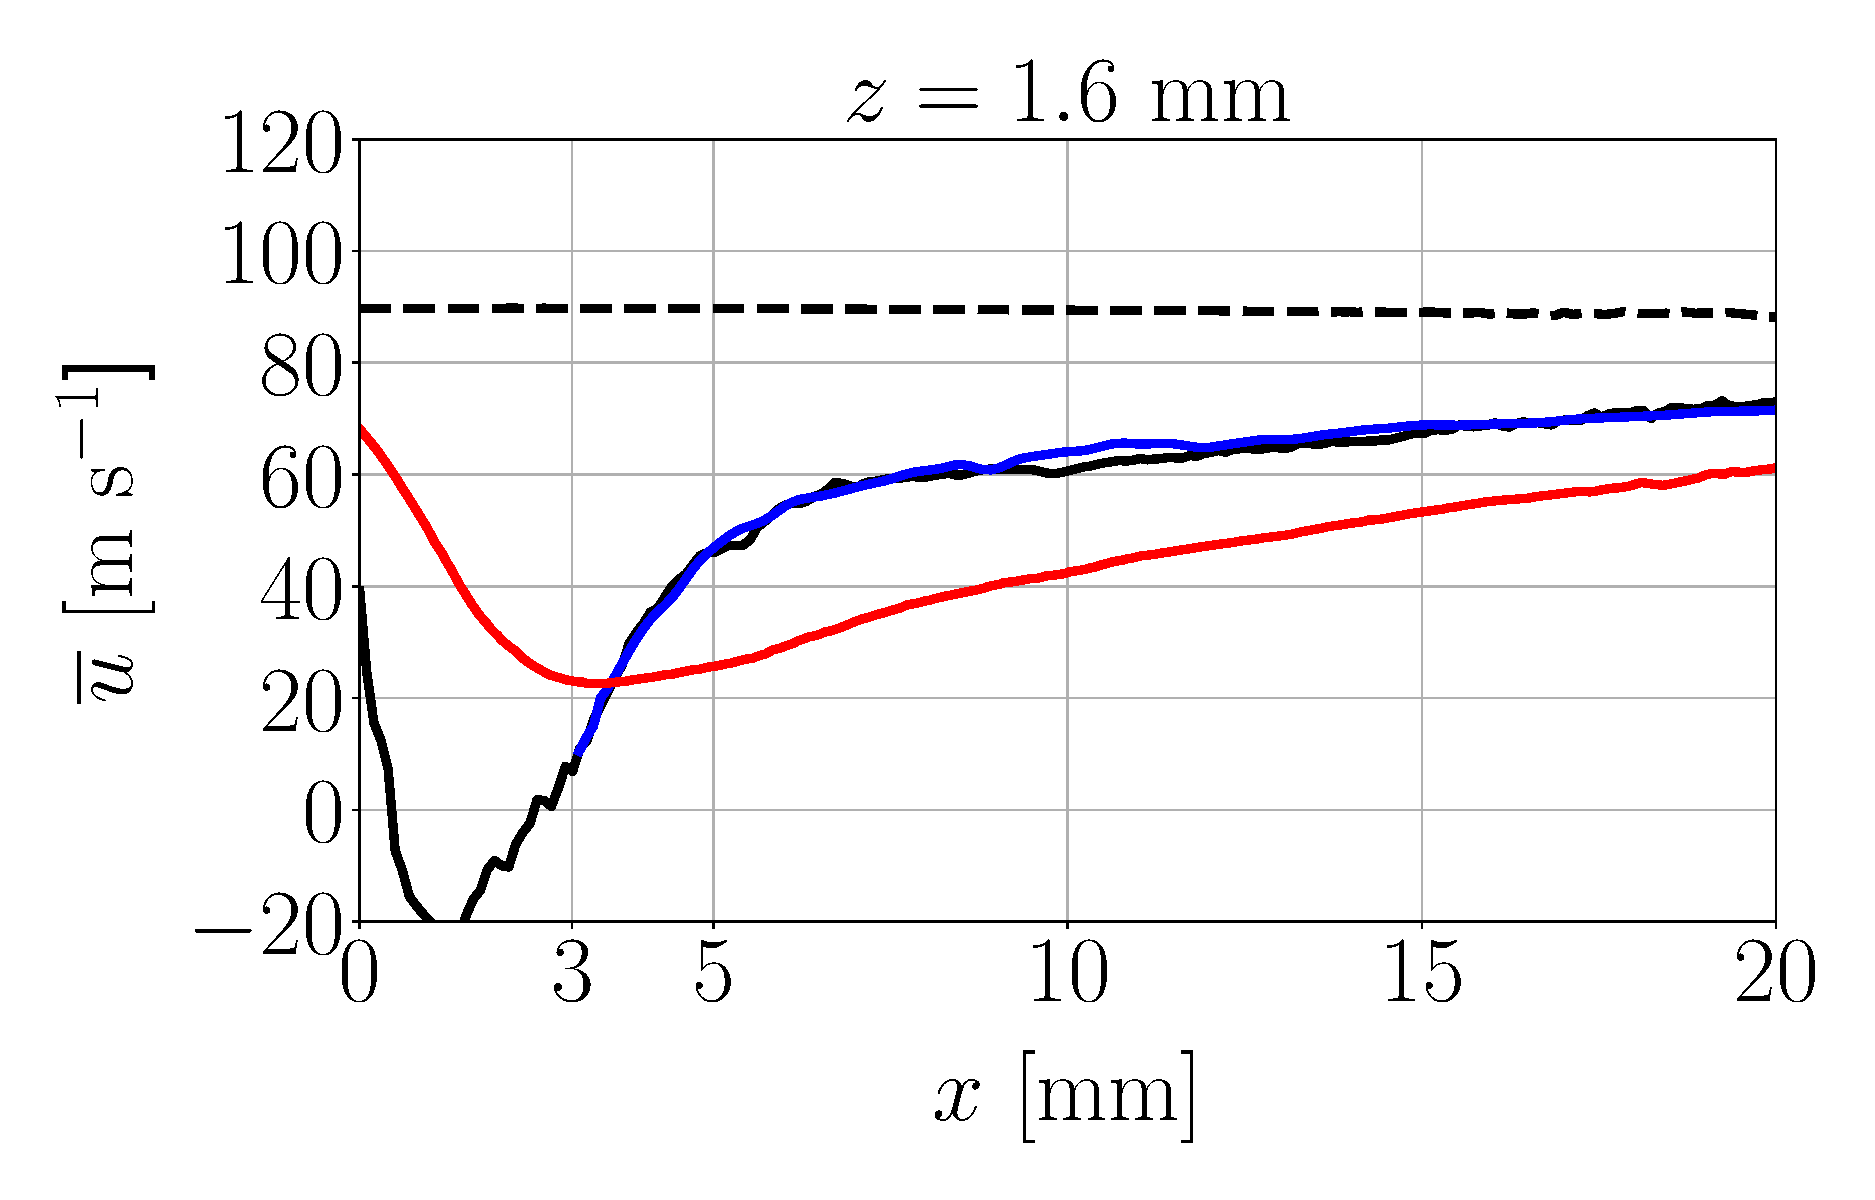
\includegraphics[scale=0.25]{./part2_developments/figures_ch6_lagrangian_JICF/gas_field_initial_conditions/custom_line_y0_along_x_z01p6}
   %\caption{}
   %\label{} 
\end{subfigure}
\hspace{0.4in}
\begin{subfigure}[b]{0.45\textwidth}
	\centering
   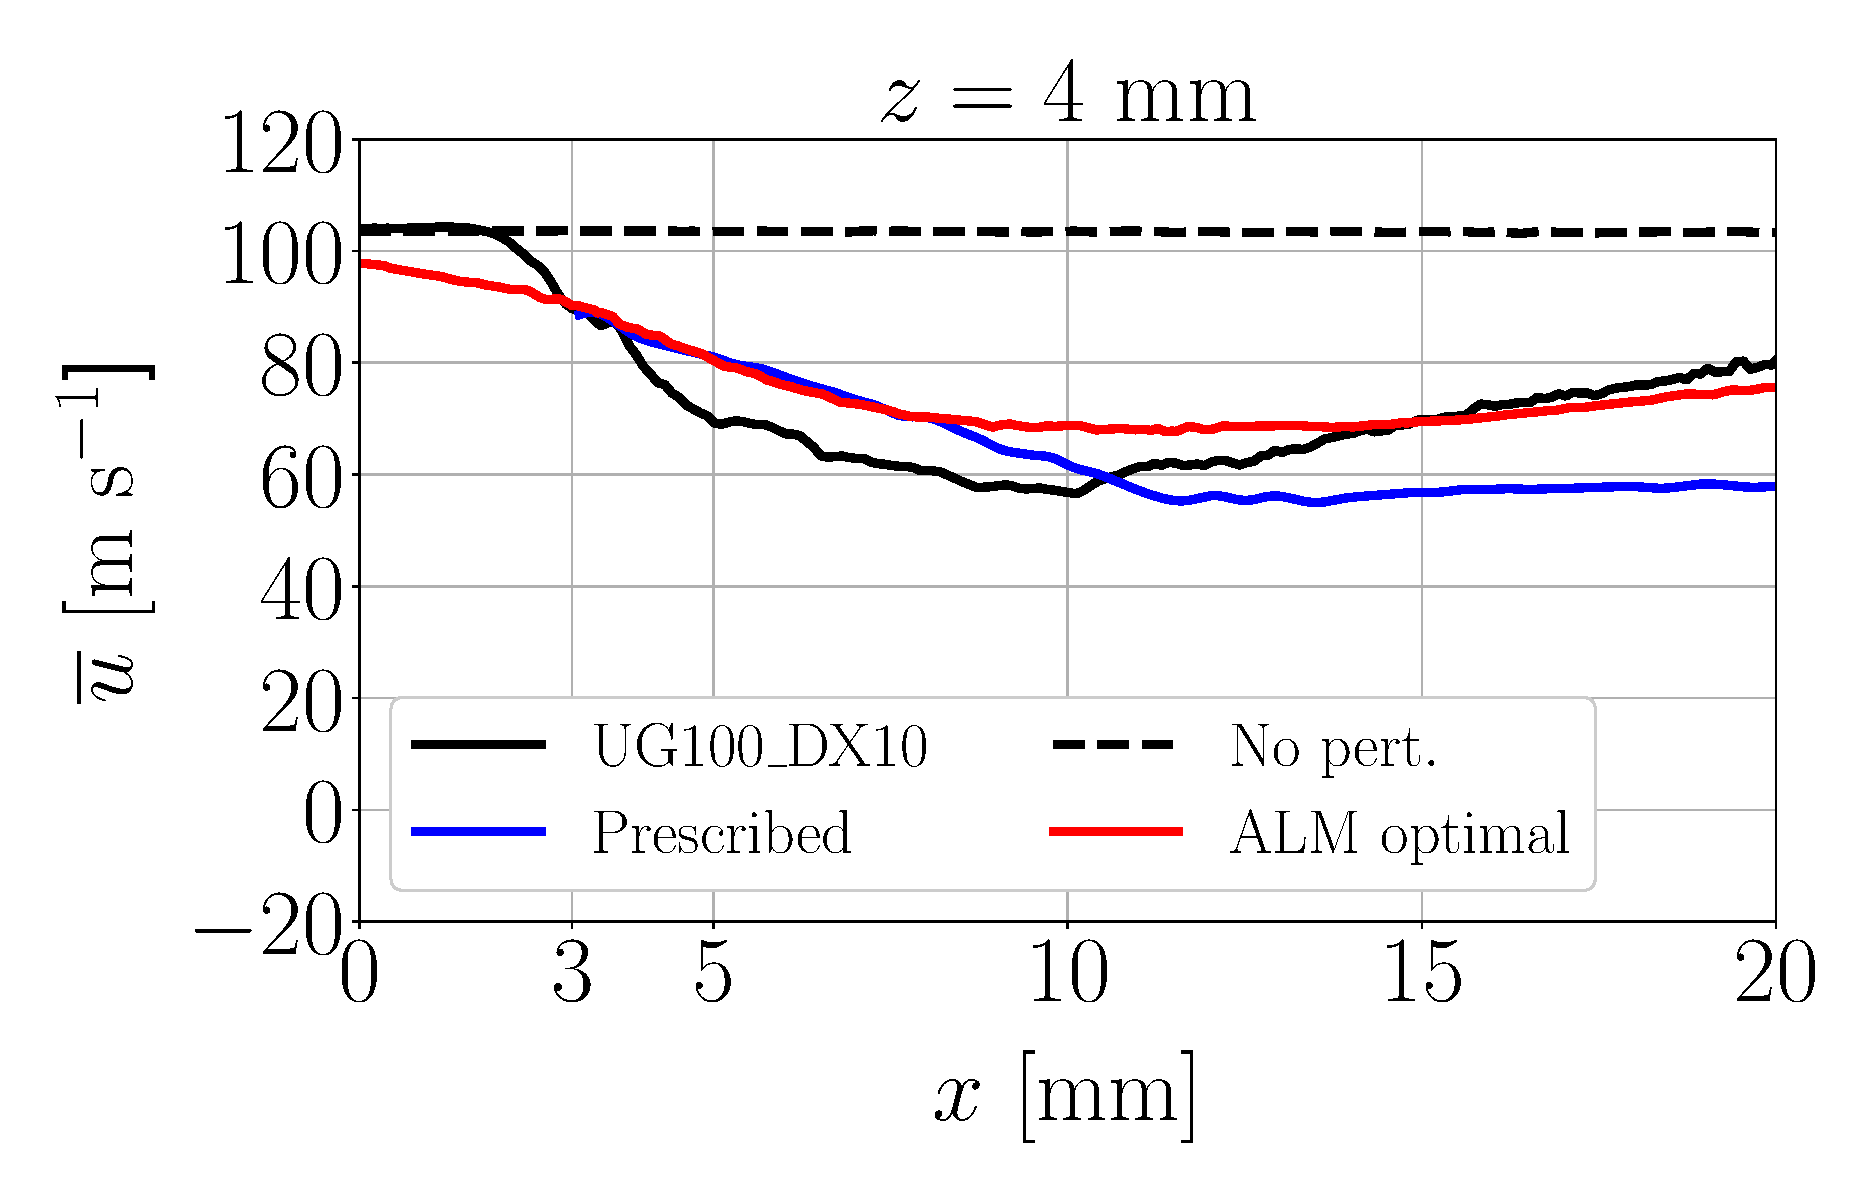
\includegraphics[scale=0.25]{./part2_developments/figures_ch6_lagrangian_JICF/gas_field_initial_conditions/custom_line_y0_along_x_z04p0}
   %\caption{}
   %\label{}
\end{subfigure}
\caption{Mean axial velocity evolution along axial coordinate at locations $z = 1.6, 4$ mm in plane $y = 0$}
\label{fig:JICF_ICS_custom_lines_y0_along_x_ux_mean}
\end{figure}

\begin{figure}[ht]
\centering
   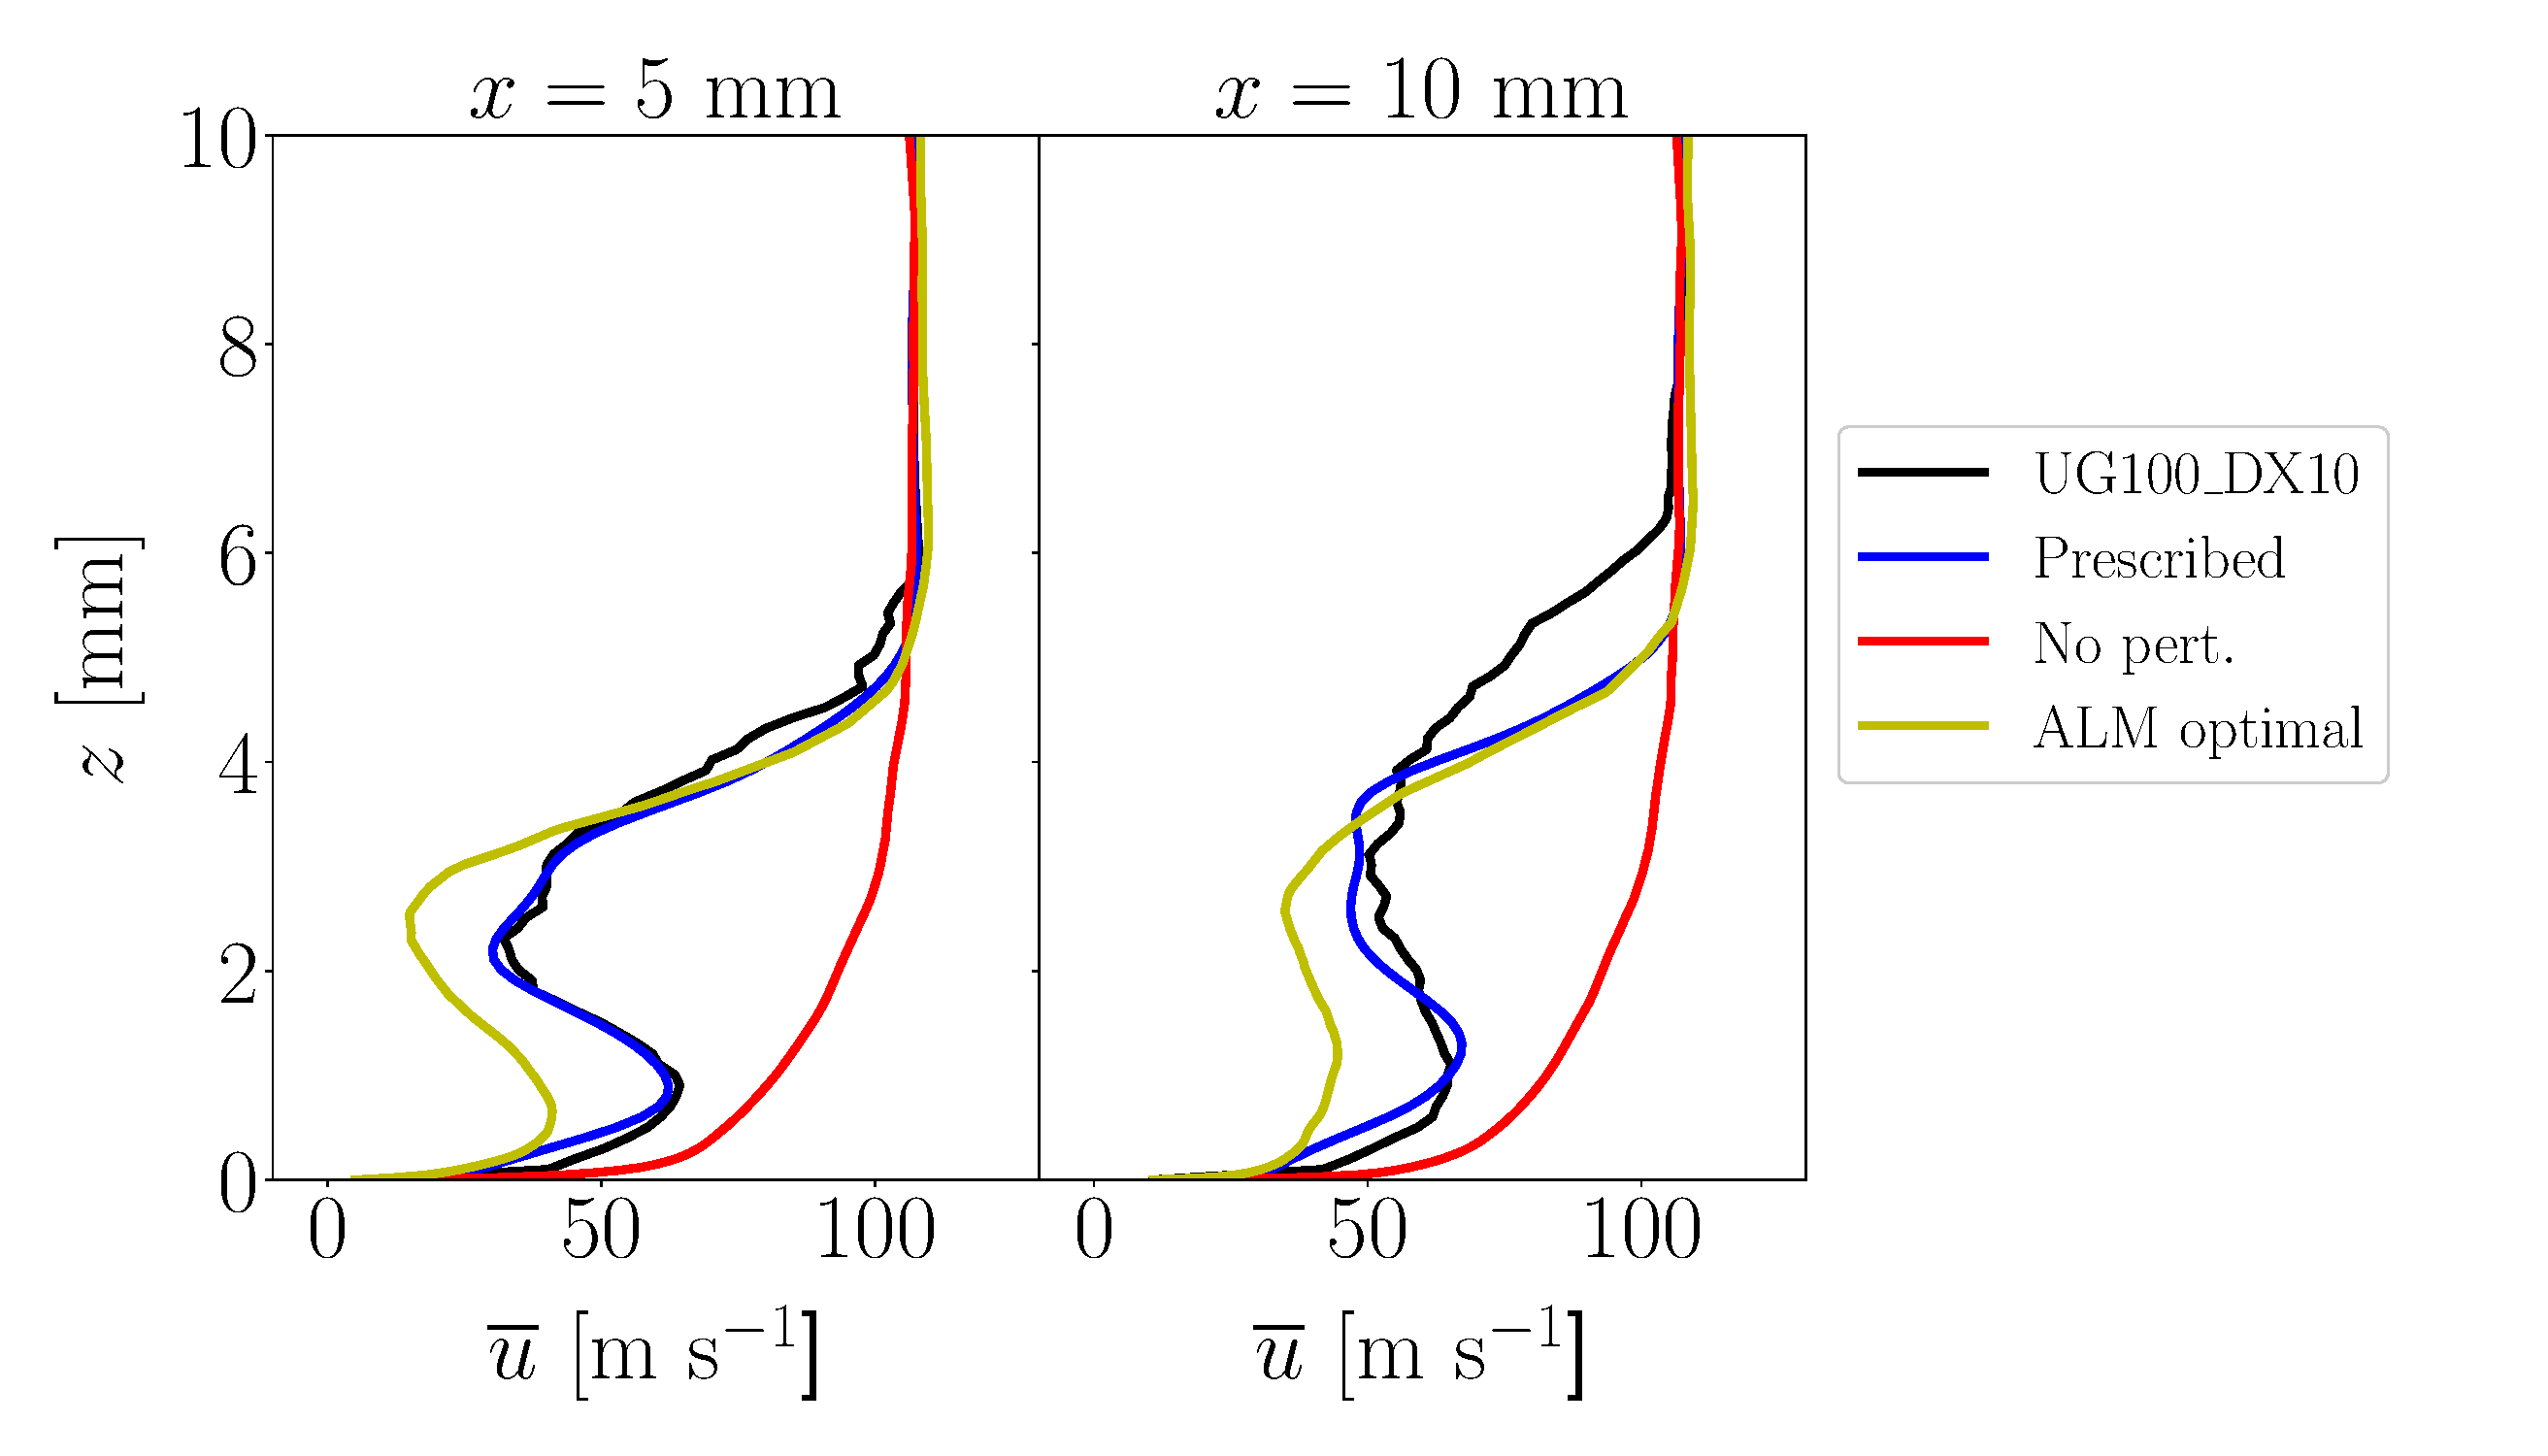
\includegraphics[scale=0.26]{./part2_developments/figures_ch6_lagrangian_JICF/gas_field_initial_conditions/custom_lines_y0_along_z_ux_mean}
\caption{Mean axial velocity evolution along vertical coordinate at $x = 2.5, 5, 10$ mm locations of plane $y = 0$ (lines of Figure \ref{fig:custom_gas_fields_plane_x}) }
\label{fig:JICF_ICS_custom_lines_y0_along_z_ux_mean}
\end{figure}
\clearpage

The flow field at planes perpendicular to crossflow direction $x = 5, 10$ mm  are displayed in Figure \ref{fig:custom_gas_fields_plane_x}. The prescribed gaseous inlet can retrieve the CRVs spinning directions in both cases. At $x = 5$ mm the vertical location of the CRV is underestimated with respect to the resolved case, while further downstream it gets closer. The velocity profiles along the white lines are shown in Figure \ref{fig:JICF_custom_lines_iso-x_along_y_ux_mean}.  Closer to the wall ($z = 1.6$ mm), the prescribed inlet profile coincides with the resolved one in all the range except for the local minima captured at both sides close to $y = 0$, which are not present in the resolved case. Further from the wall ($z = 5$ mm) the prescribed profile does not match the resolved profile due to the reasons aforementioned, and creates flow decelerations with magnitudes similar to the ALM optimal case. 

\begin{figure}[h!]	
	\centering	\includeinkscape[inkscapelatex=false,scale=0.265]{./part2_developments/figures_ch6_lagrangian_JICF/gas_field_initial_conditions/custom_inlet_planes_x}
	\caption{Mean axial velocity field at planes $x = 5, 10$ mm for resolved case UG100\_DX10 and prescribed gaseous inlet}
	\label{fig:custom_gas_fields_plane_x}
\end{figure}

\begin{figure}[ht]
\centering
\begin{subfigure}[b]{1.0\textwidth}
	\centering
   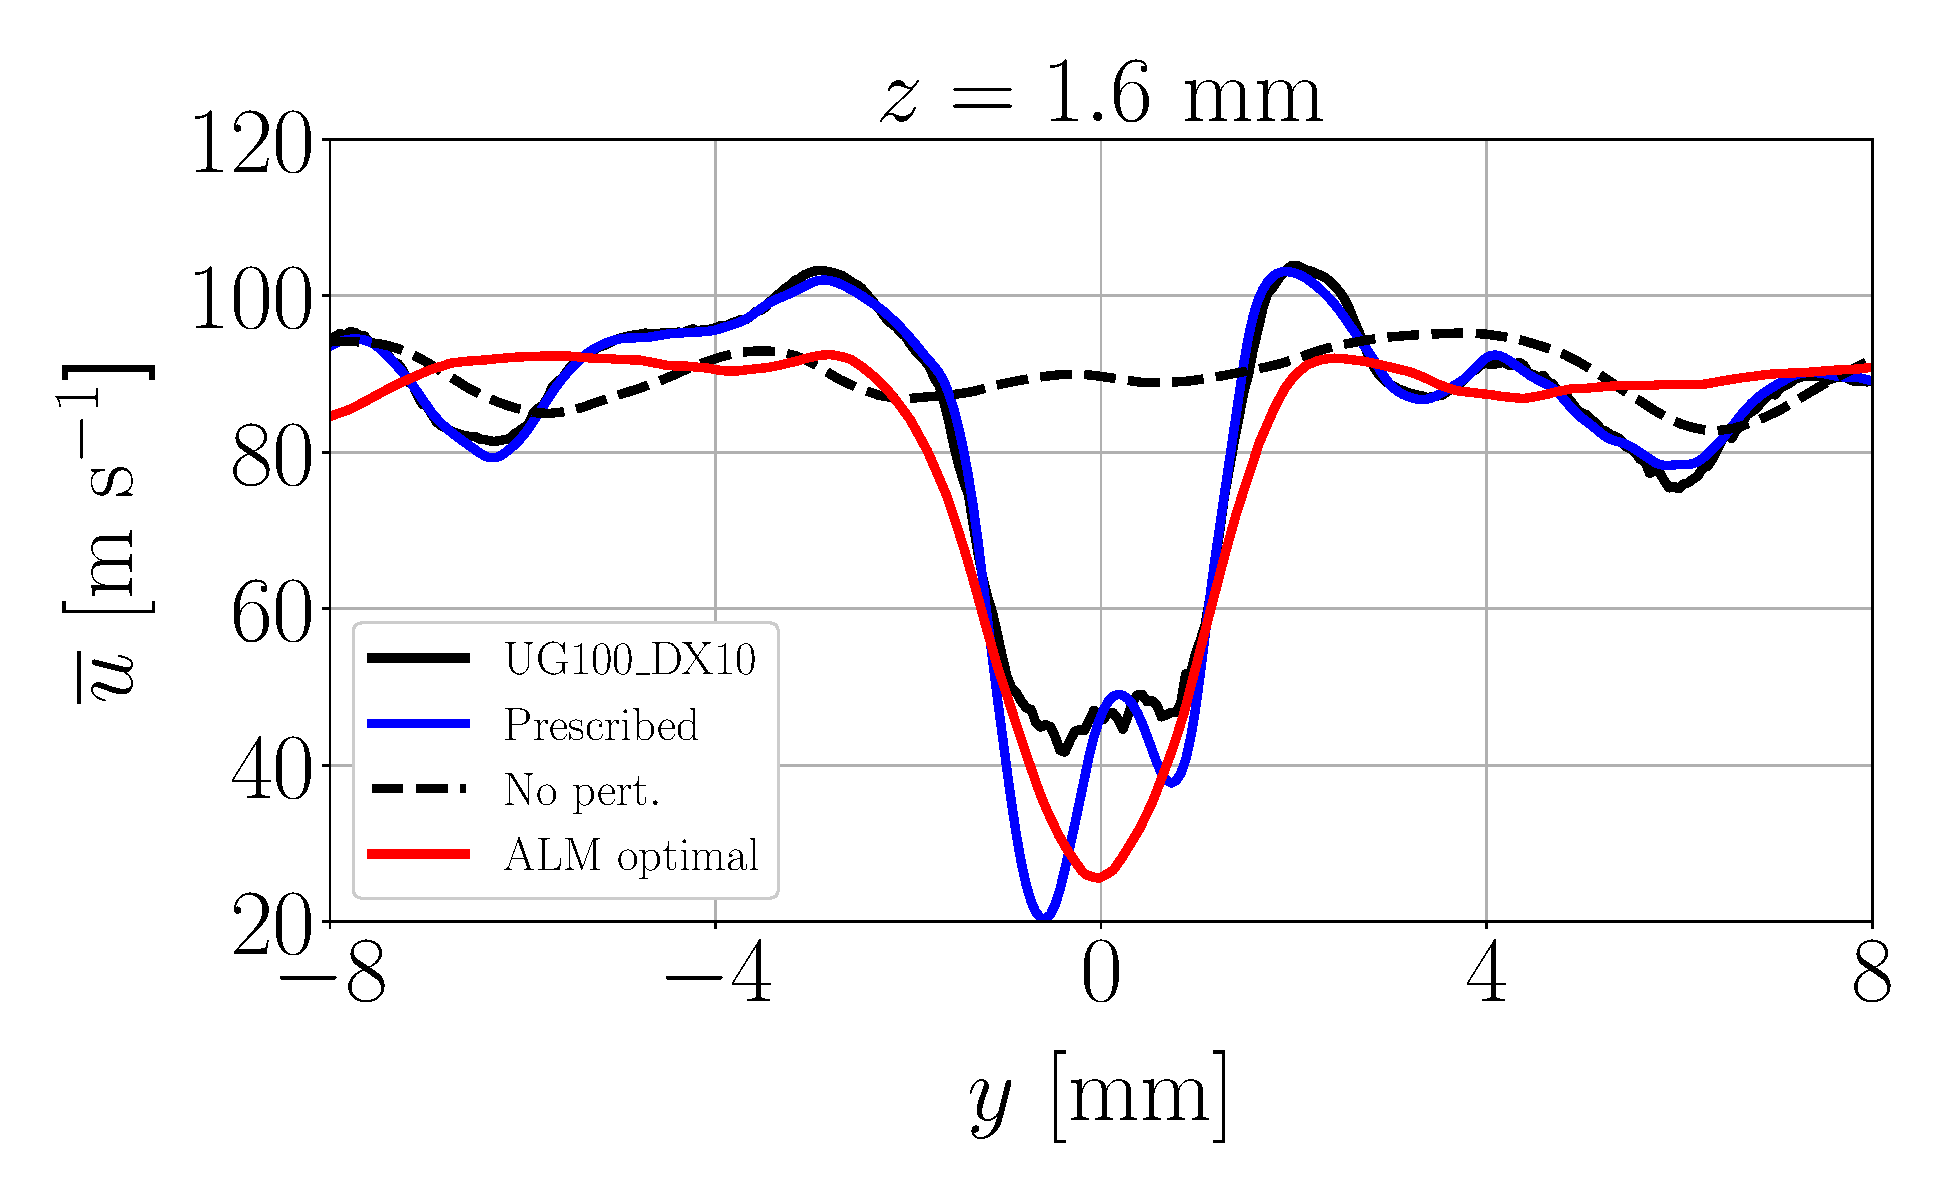
\includegraphics[scale=0.24]{./part2_developments/figures_ch6_lagrangian_JICF/gas_field_initial_conditions/custom_line_x05_z01p6_ux_mean_along_y}
   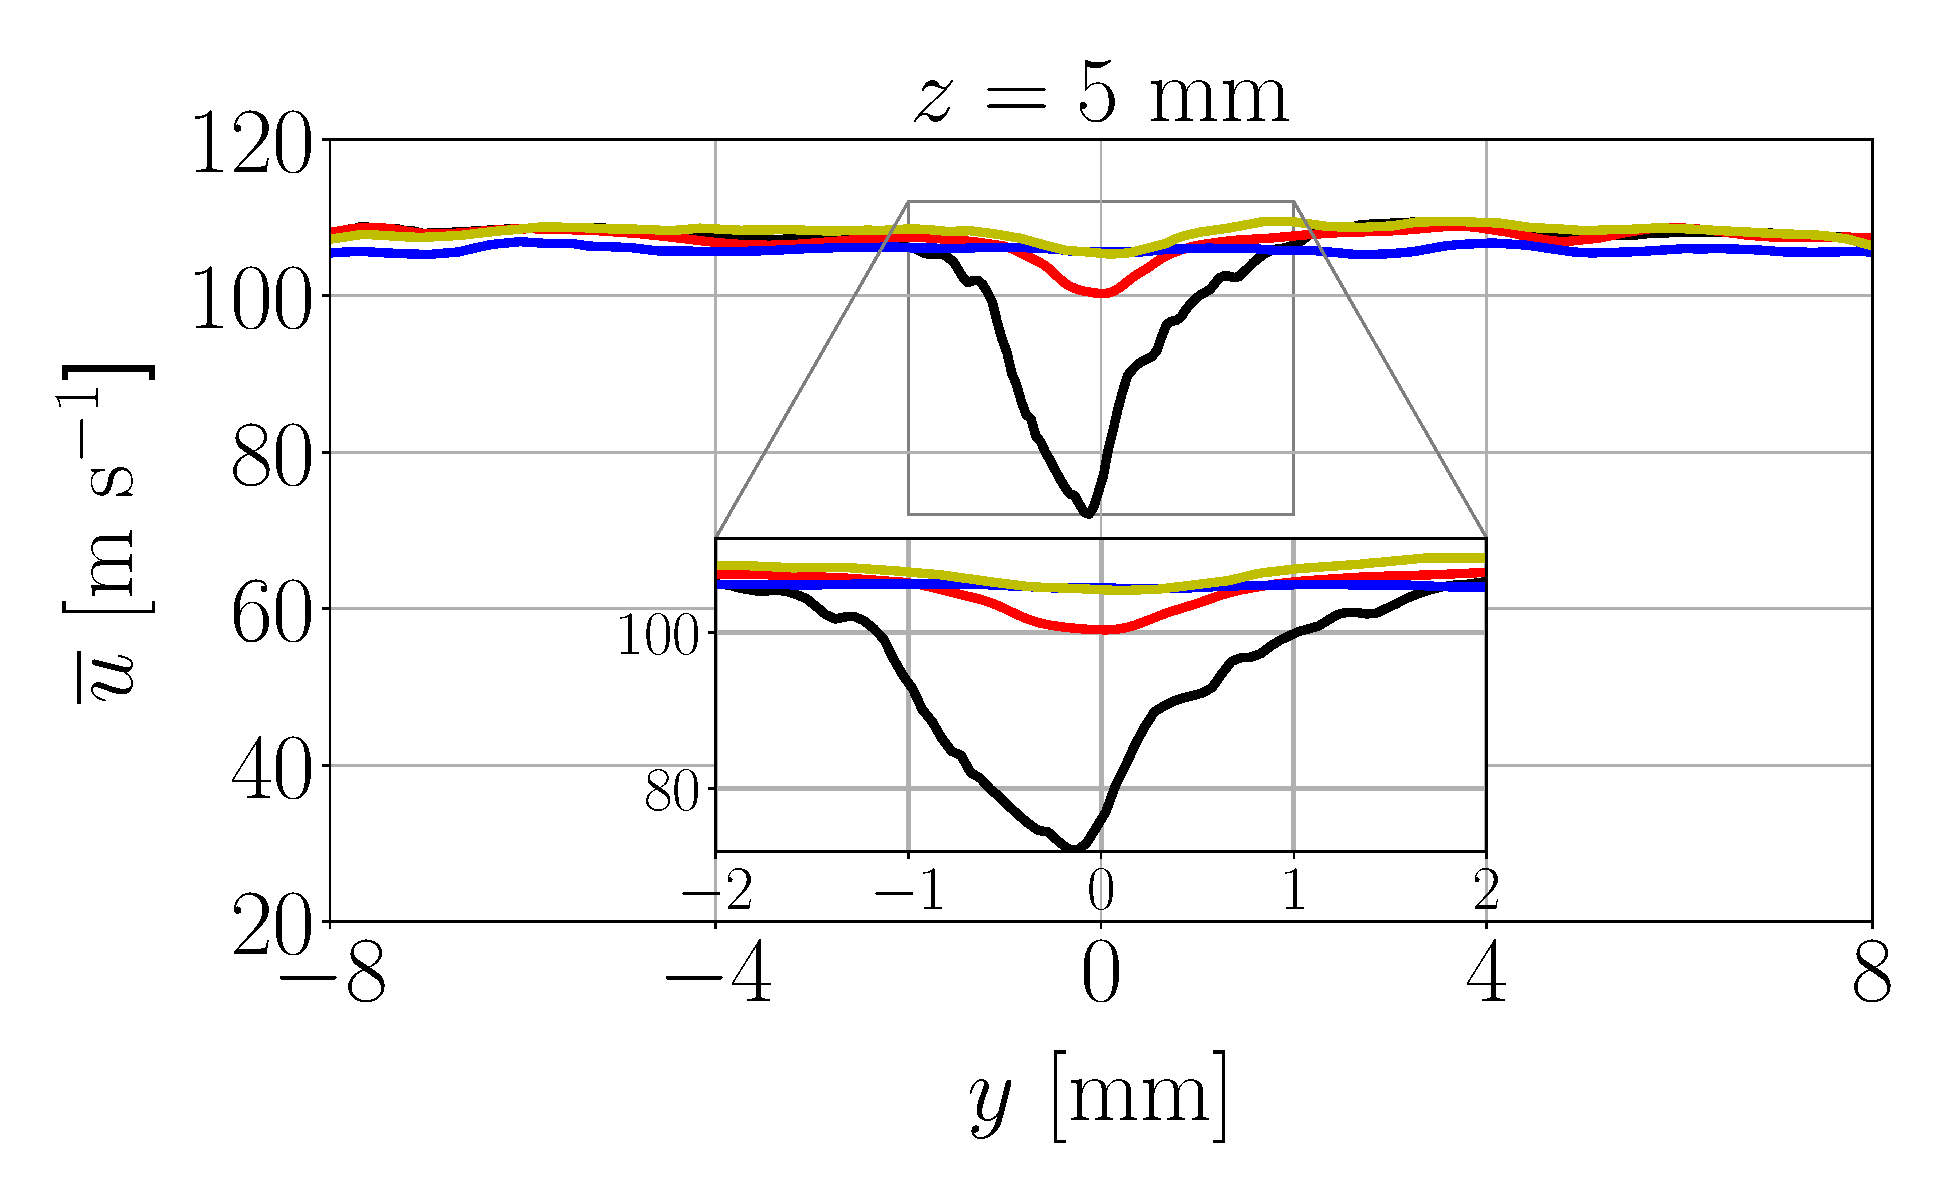
\includegraphics[scale=0.24]{./part2_developments/figures_ch6_lagrangian_JICF/gas_field_initial_conditions/custom_line_x05_z05p0_ux_mean_along_y}
   \vspace*{-0.1in}
	\caption{Plane $x = 5$ mm}
\end{subfigure}
\vskip\baselineskip
\begin{subfigure}[b]{1.0\textwidth}
	\centering
   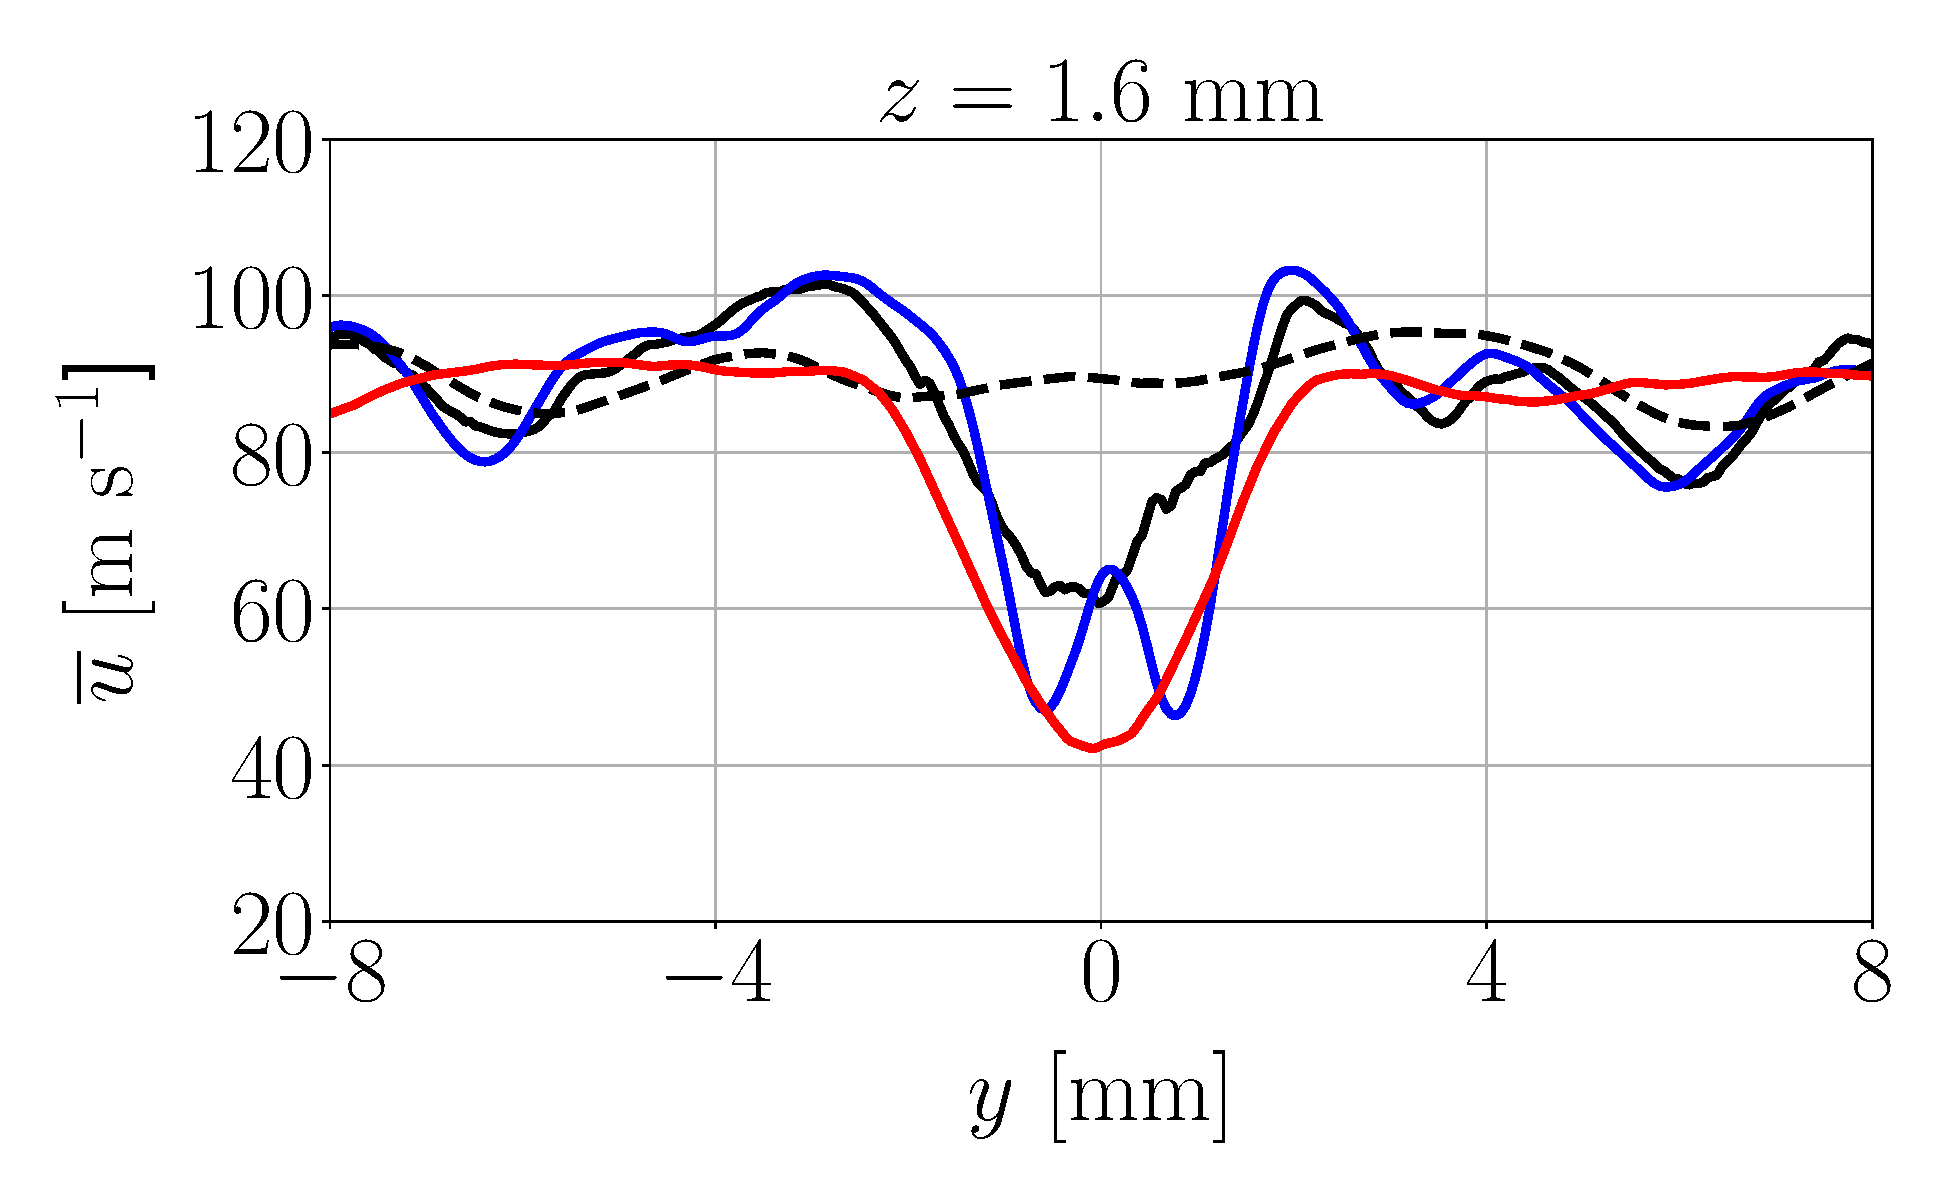
\includegraphics[scale=0.24]{./part2_developments/figures_ch6_lagrangian_JICF/gas_field_initial_conditions/custom_line_x10_z01p6_ux_mean_along_y}
   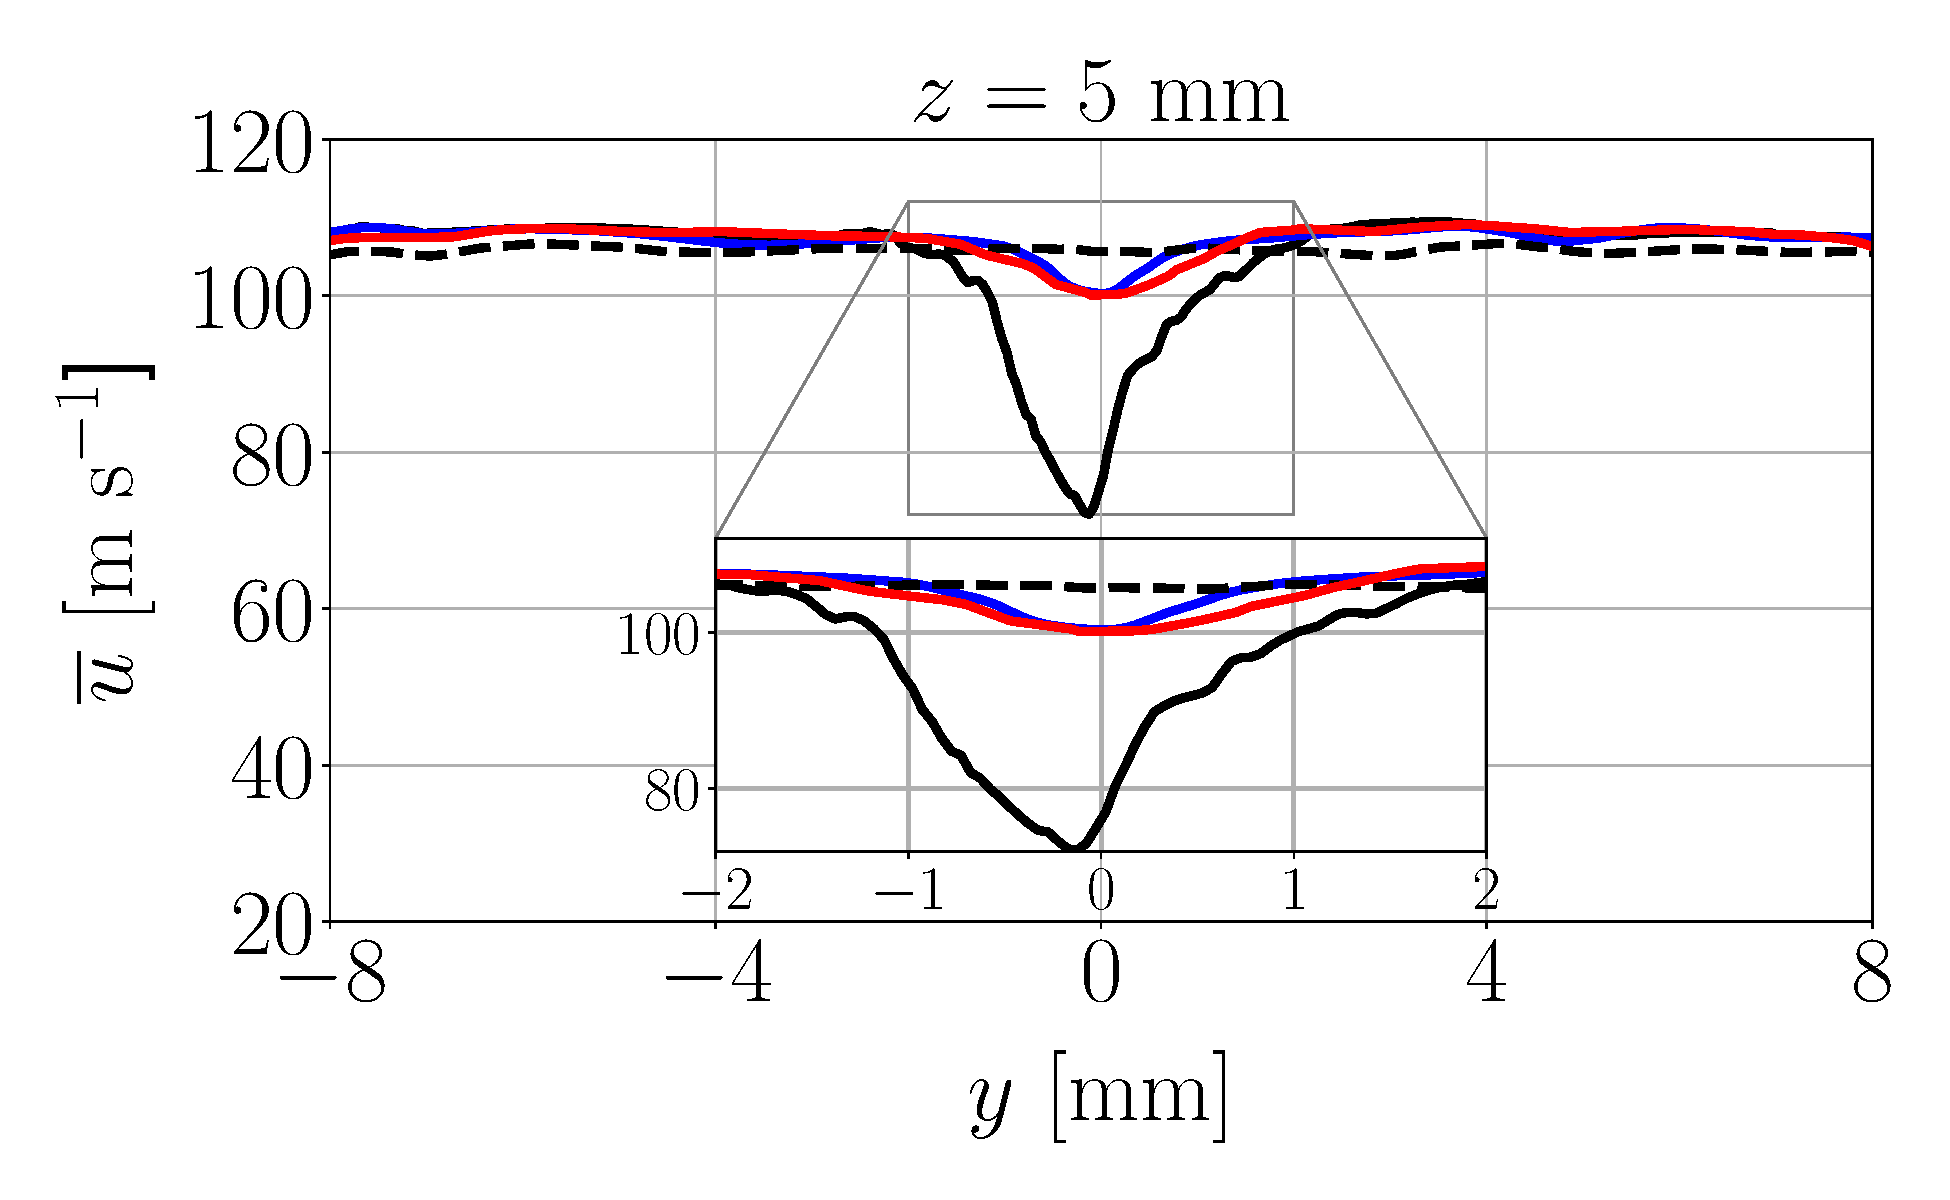
\includegraphics[scale=0.24]{./part2_developments/figures_ch6_lagrangian_JICF/gas_field_initial_conditions/custom_line_x10_z05p0_ux_mean_along_y}
   \vspace*{-0.1in}
	\caption{Plane $x = 10$ mm}
\end{subfigure}
   \caption{Mean axial velocity evolution along lateral coordinate at $z$ lines of Figure \ref{fig:custom_gas_fields_plane_x}}
\label{fig:JICF_custom_lines_iso-x_along_y_ux_mean}
\end{figure}

In general, it can be concluded that the prescribed inlet captures more accurately than the ALM tested, furthermore with lower computational cost since it represents only a portion of the original computational domain. On the contrary, the disadvantage of the prescribed inlet strategy is that it can be a priori performed in simple geometries such as the academic JICF tested. 

%\begin{figure}[ht]
%\centering
%   \includeinkscape[inkscapelatex=false,scale=0.22]{./part2_developments/figures_ch6_lagrangian_JICF/gas_field_initial_conditions/planes_y_ux_mean}
%\caption[Mean axial velocity at plane $y = 0$ mm.]{Mean axial velocity at plane $y = 0$ mm. Black lines with arrows are in-plane mean streamlines; the white solid line indicates the contour $\overline{u} = 0$ which delimites the recirculation bubble. The grey area  indicates the mean liquid region, identifed as $\overline{\psi} > 0.5$}
%\label{fig:JICF_lgs_gaseous_conditions_comparison_plane_y}
%\end{figure}
%
%
%\begin{figure}[ht]
%\centering
%   \includeinkscape[inkscapelatex=false,scale=0.18]{./part2_developments/figures_ch6_lagrangian_JICF/gas_field_initial_conditions/planes_x_ux_mean}
%\caption[Mean axial velocity at planes $x = 5, 10$ mm]{Mean axial velocity at planes $x = 5, 10$ mm. Black lines with arrows are in-plane mean streamlines.}
%\label{fig:JICF_lgs_gaseous_conditions_comparison_planes_x}
%\end{figure}



\section{Procedure for setting dispersed-phase simulations}

In Chapter \ref{ch5:jicf_resolved_simulations}, the five resolved atomization simulations from Table \ref{fig:location_JICF_ops_in_breakup_map} were performed and analyzed. These ones tested two mesh interface mesh resolutions ($\Delta x_\mathrm{min} = 20, 10~\mu$m), two operating points ($We_g = 830, 1470$) and the influence of turbulence injection in one simulation for the coarse resolution, high $We_g$ case. Results shown a high dependency of the trajectories ($\S$\ref{subsec:ch5_jet_trajectories_results}) and jet topologies ($\S$\ref{sec:ch5_jet_evolution}) on the resolution, which led later to different spray characteristics ($\S$\ref{sec:ch5_sec_spray_characterization}) and resulting injectors ($\S$\ref{sec:ch5_learning_SLI}). Therefore, it is of interest to test such effects in the disperse-phase simulations by initializing these computations with the different injectors obtained.

Figure \ref{fig:dispersed_phase_sli_parameters} shows the different models involved in the dispersed phase simulations with their control parameters: they are split into the possible influences on the gas and liquid phases, as well as the secondary breakup which is considered as an interaction between both (even though it acts on the liquid phase, it needs the gas velocity for calculating the relative velocity in order to estimate liquid breakup). In this section, all the parameters from the SLI model in the JICF case are analyzed: a baseline configuration is chosen, which was found to be the most optimal one yielding the best match to the experimental results, and then each SLI parameter is modified individually. The baseline configuration consists of the following parameters:

\begin{itemize}

	\item The \textbf{gaseous phase} is provided by the \textbf{custom inlet} methodology. This one was found to better match the aerodynamic field from the resolved computation and produces a lagrangian spray closer to the experimental results, as demonstrated in $\S$\ref{sec:SLI_LGS_gaseous_phase_effect}.
	
	\item \textbf{Secondary atomization model} is taken to be the Gorokhovski model with calibrated constants $K_1 = 0.05$, $K_2$ = 1. Calibration of the secondary model is reported in $\S$\ref{{subsec:second_atom_goro_calibration}}.
	
	\item \textbf{SLI} corresponds to the discretized spray obtained from the high Weber case at the finest resolution, UG100\_DX10, at location $x = 5$ mm. This case is chosen as the baseline one since 1) the operating point been previously studied by other authors and hence the results reported here can be easily compared ($\S$\ref{ch6:previous_numerical_studies}), 2) the finer interface cell size in the resolved simulation provides a better resolution of the sprays, and 3) the location closer to the injection point deviates less with respect to the experimental trajectory than the sampled spray further downstream (see Figure \ref{fig:JICF_trajectories_validation}). The effect of other operating conditions, resolved interface resolutions and injection locations is studied in $\S$\ref{subsec:SLI_LGS_resolution_and_injection_location},.
	
	\item \textbf{Spray velocities}: mean injection velocities are fixed to volume-weighted ones, while the $r$ law for RMS components is set to gaussian. Such parameters are analyzed in $\S$\ref{subsec:SLI_LGS_velocity_effects}.
	
	\item \textbf{Droplets sizes} prescribed are randomly sampled from a lognormal distribution fitting the histogram in each individual probe. 
	
	\item The \textbf{operating condition} is also change by performing a dispersed-phase simulation for the low Weber case with the corresponding SLI obtained. These results are reported in $\S$\hl{XX}.

\end{itemize}



\begin{figure}[h!]	
	\centering	\includeinkscape[inkscapelatex=false,scale=0.35]{./part2_developments/figures_ch6_lagrangian_JICF/chart_input_parameters_LGS}
	\caption{Schematic of parameters involved in SLI simulations and their interactions}	\label{fig:dispersed_phase_sli_parameters}
\end{figure}



With the objective of testing all the parameters involved in the lagrangian computations, a design of experiments process is followed in which each variable is changed in a one-at-a-time basis. The study of dispersed-phase simulations in then divided into three parts, which are enclosed by the dashed-colored lines in Figure  \ref{fig:dispersed_phase_sli_parameters}:

\begin{enumerate}

	\item The \textbf{gas phase} effect is analyzed by injecting lagrangian droplets with the baseline injectors in the gaseous fields previously analyzed in $\S$\ref{sec:ch6_BC_gaseous_phase}. The results are discussed in $\S$\ref{sec:SLI_LGS_gaseous_phase_effect}. In this section, the establishment of the liquid phase and time needed to convergence of mean parameters are also  included.
	
	\item The \textbf{secondary atomization models} are analyzed in $\S$\ref{sec:SLI_LGS_secondary_breakup_models}. This section is divided into two parts: a first one in which the free constants of the Gorokhovski model are tuned, and a second one in which the three available. models are compared.
	
	\item Finally, the effects of the \textbf{liquid phase} parameters from SLI and operating conditions are reported in $\S$\ref{sec:effect_of_SLI_variables}. Besides the already introduced parameters, a last variable which consists of a spatial delay in which secondary atomization is not activated $\Delta x_\mathrm{atom}$ is also discussed.

\end{enumerate}




\section{Influence of gas phase}
\label{sec:SLI_LGS_gaseous_phase_effect}

\subsection{Lagrangian jet establishment}

The establishment of the dispersed phase for cases ALM optimal and the prescribed inlet are shown in Figure \ref{fig:JICF_LGS_spray_establishment}. In both cases  the injection and experimental validation planes, $x = 5$ and $x = 80$ mm respetively, are shown, as well as the liquid injection region enclosed by the black outline in the injection plane. For the case with ALM, the actuator is represented by the denoted cylinder. The prescribed inlet simulation includes as well an instantaneous view of the resolved liquid jet from case UG100\_DX10 solely for visualization among resolved and lagrangian jets: resolved liquid is not actualy present in the dispersed-phase computations. The time instants are expressed in a dimensionless form with respect to the inertial timescale according to Eq. (\ref{eq:t_dimensionless_with_tau_in}).

In both simulations, lagrangian droplets are injected in the denoted liquid injection region (which represents the spatial bounds of the SLI from Figure \ref{fig:injectors_sli_uG100_dx10_x05}) which are then convected downstream. Right after injection, the particles have a diameter of the order of the SMD from Figure \ref{fig:injectors_sli_uG100_dx10_x05} and a finite vertical component velocity which is lower at the bottom of the injection plane and larger at its tope. As a consequence of this vertical velocity component, the jet's vertical trajectory continues to increase with axial distance. Shortly after injection, droplets are quickly atomized into smaller particles due to the action of the secondary breakup model. The liquid-gas relative velocity is large in all simulations, hence the breakup model estimates the atomization events to occur soon after injection and the size of the droplets is reduced very fast with axial distance. The atomization region has been found to extend up to \hl{10 mm downstream the injection} location, as quantified later in $\S$\ref{subsec:jicf_lgs_sed_gas_phase_influence_spray_analysis}. Downstream this location the dispersed spray is fully atomized and droplets are only convected. As a consequence of such a fast breakup, the smaller droplets generated have a lower relaxation time and are quickly dragged by the gaseous crossflow, increasing their axial velocity and reducing their vertical one, hence stopping penetrating in the vertical direction. 

Figure \ref{fig:JICF_LGS_spray_establishment} shows the secondary atomization of a single lagrangian droplet in case ALM initial. The displayed domain in each figure corresponds to the region enclosed by the red rectangle in Figure \ref{fig:JICF_LGS_spray_establishment}. Then, further zoomed views enclosed in blue show the droplets generated from the original droplet detected at the firstly displayed time instant. The original droplet at $t^* = 22.40$, with a diameter of 93 $\mu$m, breaks into several droplets of smaller size at $t^* = 23.02$ whose total volume contains the same mass as the original droplet. These children droplets have different sizes as a consequence of the statistical sampling from the cumulative distribution Eq. (\ref{eq:gorokhovski_T_CDF}). Particles are then convected and undergo a further breakup event at $t^* = 24.26$, producing a larger number of smaller children droplets, where the smallest diameter produced was 13 $\mu$m. This sequence of subsequent atomization events is referred as the breakup cascade mechanism \citepColor[tanner_simulation_1998]. In the particular snapshots shown, the original droplet prior to breakup at $t^* = 22.4$ is located at $x = 5.5$ mm (i.e. 0.5 mm further downstream the injection location), while the droplets at the last instant $t^* = 24.26$ are located at $x \sim 9$ mm. This indicates that the breakup cascade occurs soon after the injection process and gets completed shortly afterwards: in this particular case, the breakup cascade occurs within a region $\Delta x = 3.5$ mm in a timespan of $\Delta t^* = 1.86$, which corresponds to a physical timespan of $\Delta t = 0.036$ ms. 

\clearpage


\begin{figure}[h!]
	\centering	\includeinkscape[inkscapelatex=false,scale=0.8]{./part2_developments/figures_ch6_lagrangian_JICF/jet_establishment/JICF_LGS_establishment}
	\caption[Lagrangian jet establishment in the JICF simulation performed for the ALM optimal and prescribed inlet gaseous phases]{Lagrangian jet establishment in the JICF simulation performed for the ALM optimal and prescribed inlet gaseous phases. The former denotes the actuator region by the cylinder sketch, while the latter displays the liquid jet from the resolved computation only for visual comparison, since this jet is not actually present in the dispersed-phase comptutation. The region enclosed by the blue rectangle at instant $t^* = 21.78$ for case ALM initial is augmented in Figure \ref{fig:JICF_LGS_breakup_cascade_in_ALM_figure} to illustrate the breakup sequence of a single lagrangian droplet. Each sphere represents a parcel containing three droplets with the displayed diameter. Each sphere is scaled by 3 times its diameter for better visualization}
	\label{fig:JICF_LGS_spray_establishment}
\end{figure}

\clearpage

\begin{figure}[h!]
	\centering	\includeinkscape[inkscapelatex=false,scale=0.8]{./part2_developments/figures_ch6_lagrangian_JICF/jet_establishment/JICF_LGS_breakup_cascade_in_ALM}
	\caption[Visualization of the breakup cascade from a single lagrangian droplet in case ALM initial illustrating the breakup cascade]{Visualization of the breakup cascade from a single lagrangian droplet in case ALM initial illustrating the breakup cascade. Displayed domain at each instant corresponds to the region enclosed in red at Figure \ref{fig:JICF_LGS_spray_establishment}}
	\label{fig:JICF_LGS_breakup_cascade_in_ALM_figure}
\end{figure}

\subsection{Analysis of lagrangian spray}
\label{subsec:jicf_lgs_sed_gas_phase_influence_spray_analysis}

\subsubsection*{Spray establishment}

The resulting dispersed-phase sprays can be analyzed by tracking lagrangially the droplets when they cross planes perpendicular to the gaseous crossflow in the same way as performed in the resolved atomization simulations. The difference with respect to the latter is that each lagrangian droplet is identified with a unique tag that allows to detect if a lagrangian droplet has been previously sampled or not.  In this way, particles that might be tracked more than once with the detection algorithm are only accounted in the first time instant detected, hence avoiding repeated droplets when processing the spray. The only case in which this fails is if the atomization models triggers a breakup event when a parent droplet is crossing a sampling plane, since children droplets are given a new tag that fails in the detection of \textsl{repeated droplets} in such case.

Sprays have been sampled in planes perpendicular to the crossflow direction separated by a distance $\Delta x = 2$ mm from the injection location $x = 5$ mm up to the experimental sampling plane $x = 80$ mm, both shown in Figure \ref{fig:JICF_LGS_spray_establishment}. In order to study established sprays, the time that the first droplet takes to reach the experimental sampling plane $x = 80$ mm, hereafter referred as $\tau_\mathrm{dr_{x=80}}$, has been firstly obtained. Then, simulations have been run for a time $t \sim 2 \tau_\mathrm{dr_{x=80}}$ (establishment time) without lagrangian droplets tracking, and then tracking has been activated and statistics have started to be calculated. The times $\tau_\mathrm{dr_{x=80}}$ for the gaseous simulations performed are summarized in Table \ref{tab:jicf_LGS_t_prime_accumulation}, which are very close among all cases simulated. The convergence of the global spray has then be assessed by monitoring the SMD and the flux $Q_l$ with respect to time, which is expressed in a dimensionless form with respect to $\tau_\mathrm{dr_{x=80}}$ as:

\begin{equation}
\label{eq:t_prime_with_tau_drx80}
t^{\prime} = \frac{t}{\tau_\mathrm{dr_{x=80}}}
\end{equation}

Figure \ref{fig:LGS_QL_and_SMD_convergence_with_time} shows the evolution of liquid flux and SMD with time.\hl{As seen ...}.




\begin{table}[!h]
\centering
\caption{Droplets arrival time to $x = 80$ mm, total physical $t_\mathrm{ph}$ and accumulation times $t_\mathrm{acc}$, absolute and dimensionless with Eq. (\ref{eq:t_prime_with_tau_drx80}), for lagrangian JICF simulations}
\begin{tabular}{cccccc}
\thickhline
\textbf{Case} & $\tau_\mathrm{dr_{x=80}}$ & $t_\mathrm{ph}~[\mathrm{ms}]$ &  $t_\mathrm{ph}^{\prime}$ & $t_\mathrm{acc}~[\mathrm{ms}]$  & $t_\mathrm{acc}^{\prime}$  \\
\hline
Prescribed inlet & 0.7017 &  &  &  & \\
No ALM & 0.6936 &  &  &  & \\
ALM initial & 0.6959 & &  &  & \\
ALM modified (F = 0.1) & 0.6829 &  &  &  &  \\
ALM optimal (F = 0.24) & 0.6843 &  &  &  &  \\
ALM modified (F = 0.30) & 0.6812 &  &  &  &  \\
\thickhline
\end{tabular}
\label{tab:jicf_LGS_t_prime_accumulation}
\end{table}

\clearpage

\begin{figure}[ht]
\flushleft
\begin{subfigure}[b]{0.45\textwidth}
	\centering
   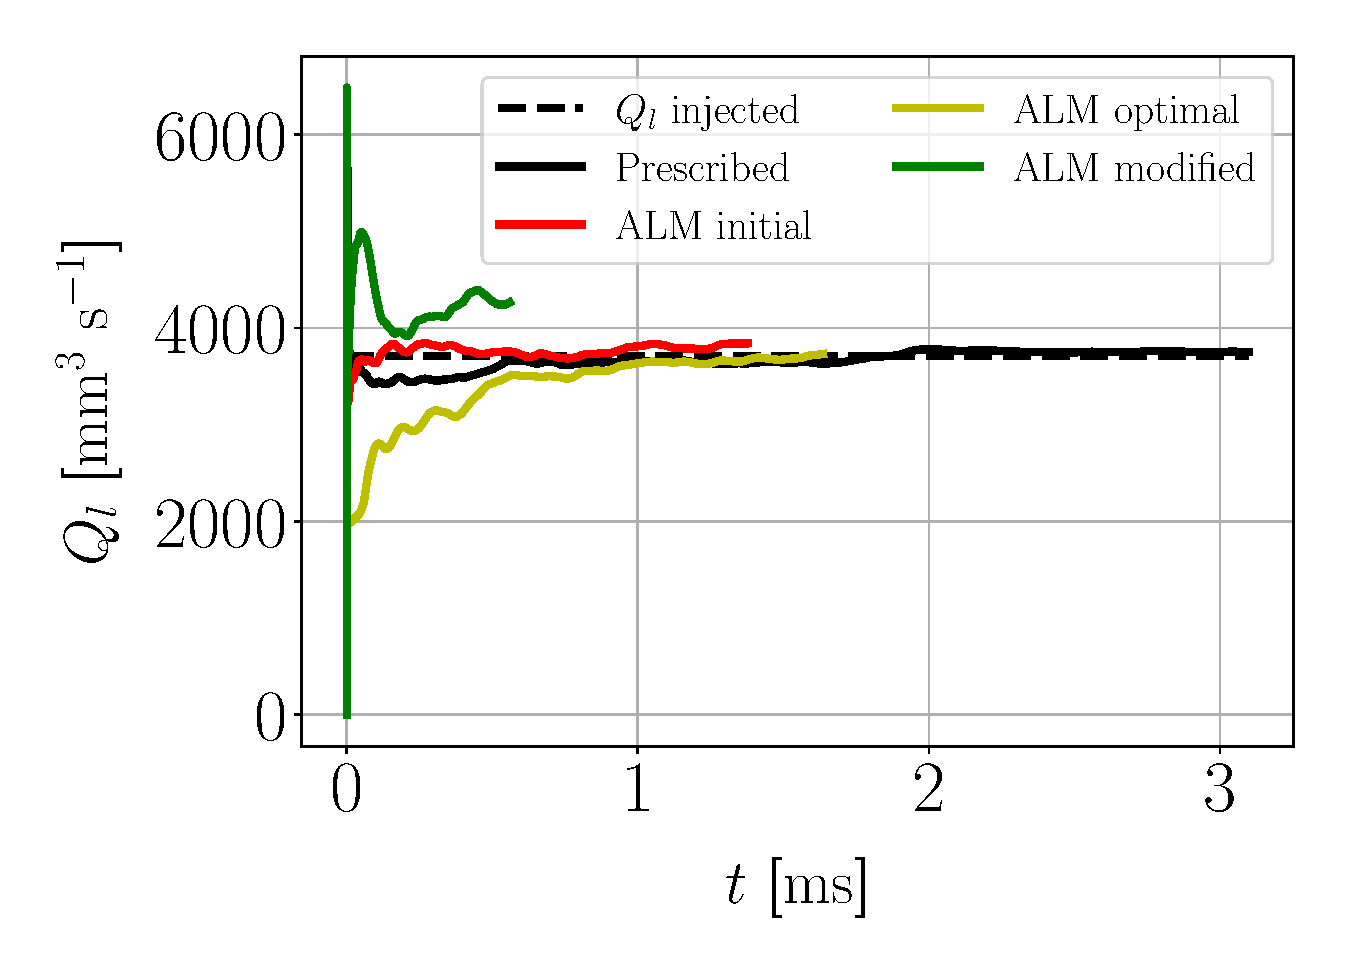
\includegraphics[scale=0.36]{./part2_developments/figures_ch6_lagrangian_JICF/params_gaseous_initial_conditions/convergence_Ql}
   %\caption{}
   %\label{} 
\end{subfigure}
\hspace{0.4in}
\begin{subfigure}[b]{0.45\textwidth}
	\centering
   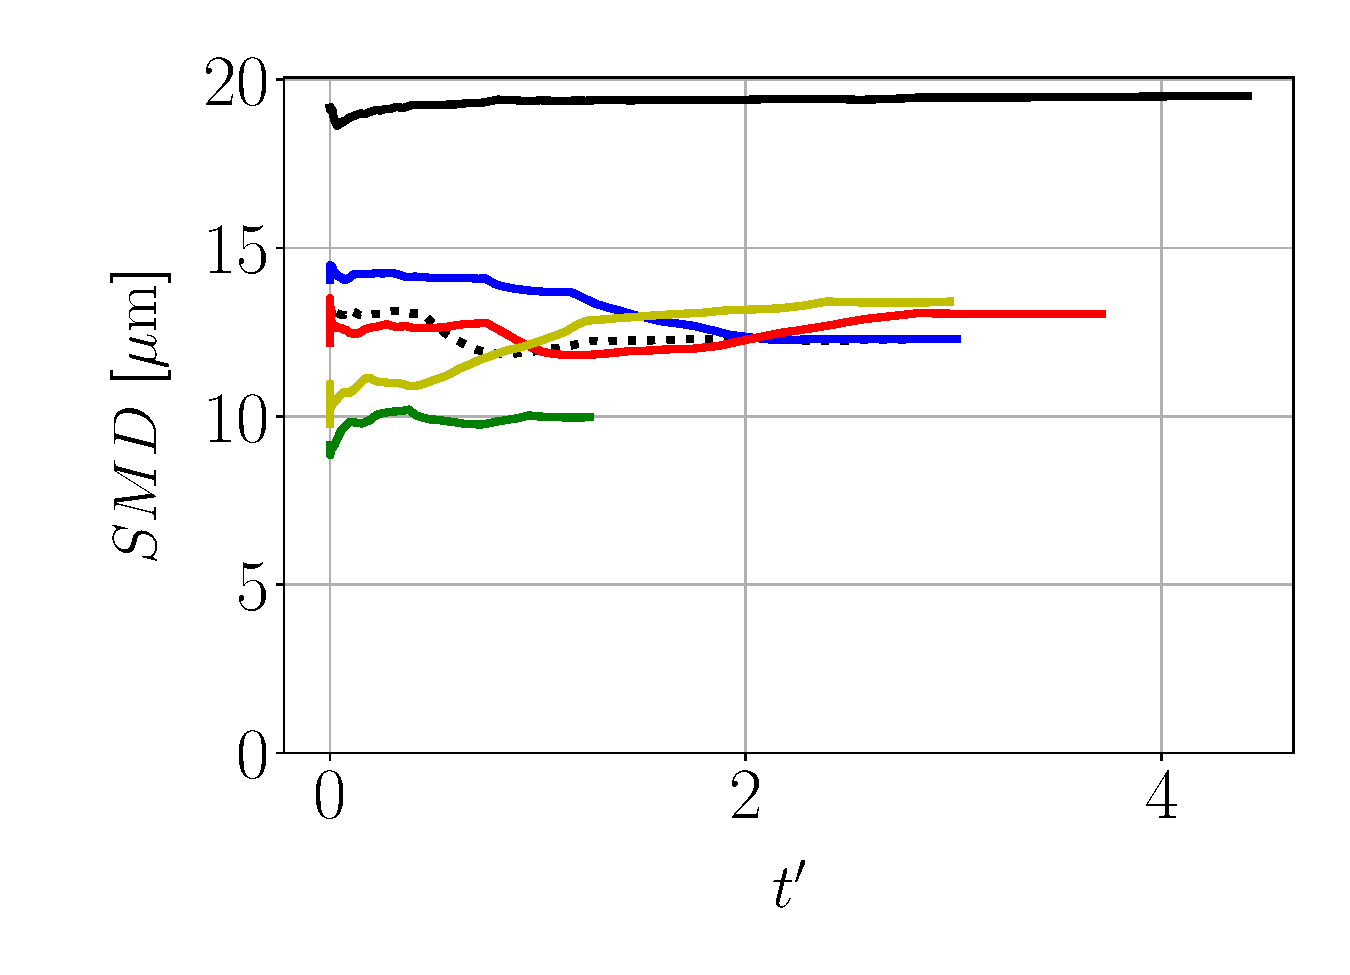
\includegraphics[scale=0.36]{./part2_developments/figures_ch6_lagrangian_JICF/params_gaseous_initial_conditions/convergence_SMD}
   %\caption{}
   %\label{}
\end{subfigure}
\caption{Convergence of spray liquid flux (\textsl{left}) and SMD (\textsl{right}) with time at plane $x = 80$ mm}
\label{fig:LGS_QL_and_SMD_convergence_with_time}
\end{figure}

\subsection*{Spatial evolution of spray}

Prior to compare the numerical results with the experimental data at $x = 80$ mm, it is interesting to see the extent at which the spray is atomized or not, since the $SMD$ graph from Figure \ref{fig:LGS_QL_and_SMD_convergence_with_time} shows low values compared to the injected $SMD$ of \hl{XX}. For this purpose, the evolution of $SMD$ with axial distance from the injection location until the experimental plane is plotted in Figure \ref{fig:SMD_vs_x_param_gaseous_BCs}. The $SMD$ from the resolved simulation UG100\_DX10 and the experimental one with the uncertainty estimated in $\S$\ref{sec:jicf_dlr_experimental_uncertainty} are also shown for comparison. As observed, the $SMD$ drops drastically shortly after injection and reaches a stable position at $x \sim 15$ mm, then it stays constant for the prescribed inlet case and it keeps decreasing linearly with $x$ for the ALM cases. The abrupt decrease in diameter at early axial locations is exponential and shows a similar shape for all cases;  however, the decaying rate and the final $SMD$ at which the dispersed-phase stabilizes depends on the case. In general, the prescribed inlet provides the largest $SMD$ while the ALM cases result in lower values due to a worse replication of the resolved gaseous phase, thus mispredicting the relative velocity for the lagrangian droplets and affecting breakup. At $x = 10$ mm the deviation with the resolved case is large: \hl{XX} vs \hl{XX} for the prescribed inlet, which supposes a difference of \hl{XX} $\%$ (however, it is worth to remind that the resolved atomization simulation might not be fine enough to resolve the smallest liquid scales that would be actually present as discussed in $\S$\ref{ch5:subsec_spray_char_granulo}, hence limiting the smallest droplets that can be obtained with the resolution employed). Further downtream at $x= 80$ mm, the numerical diameters obtained are of the order of the experimental $SMD$ of 31 $\mu$m, but yet they underestimate this value. 

\clearpage

\begin{figure}[h!]
\centering
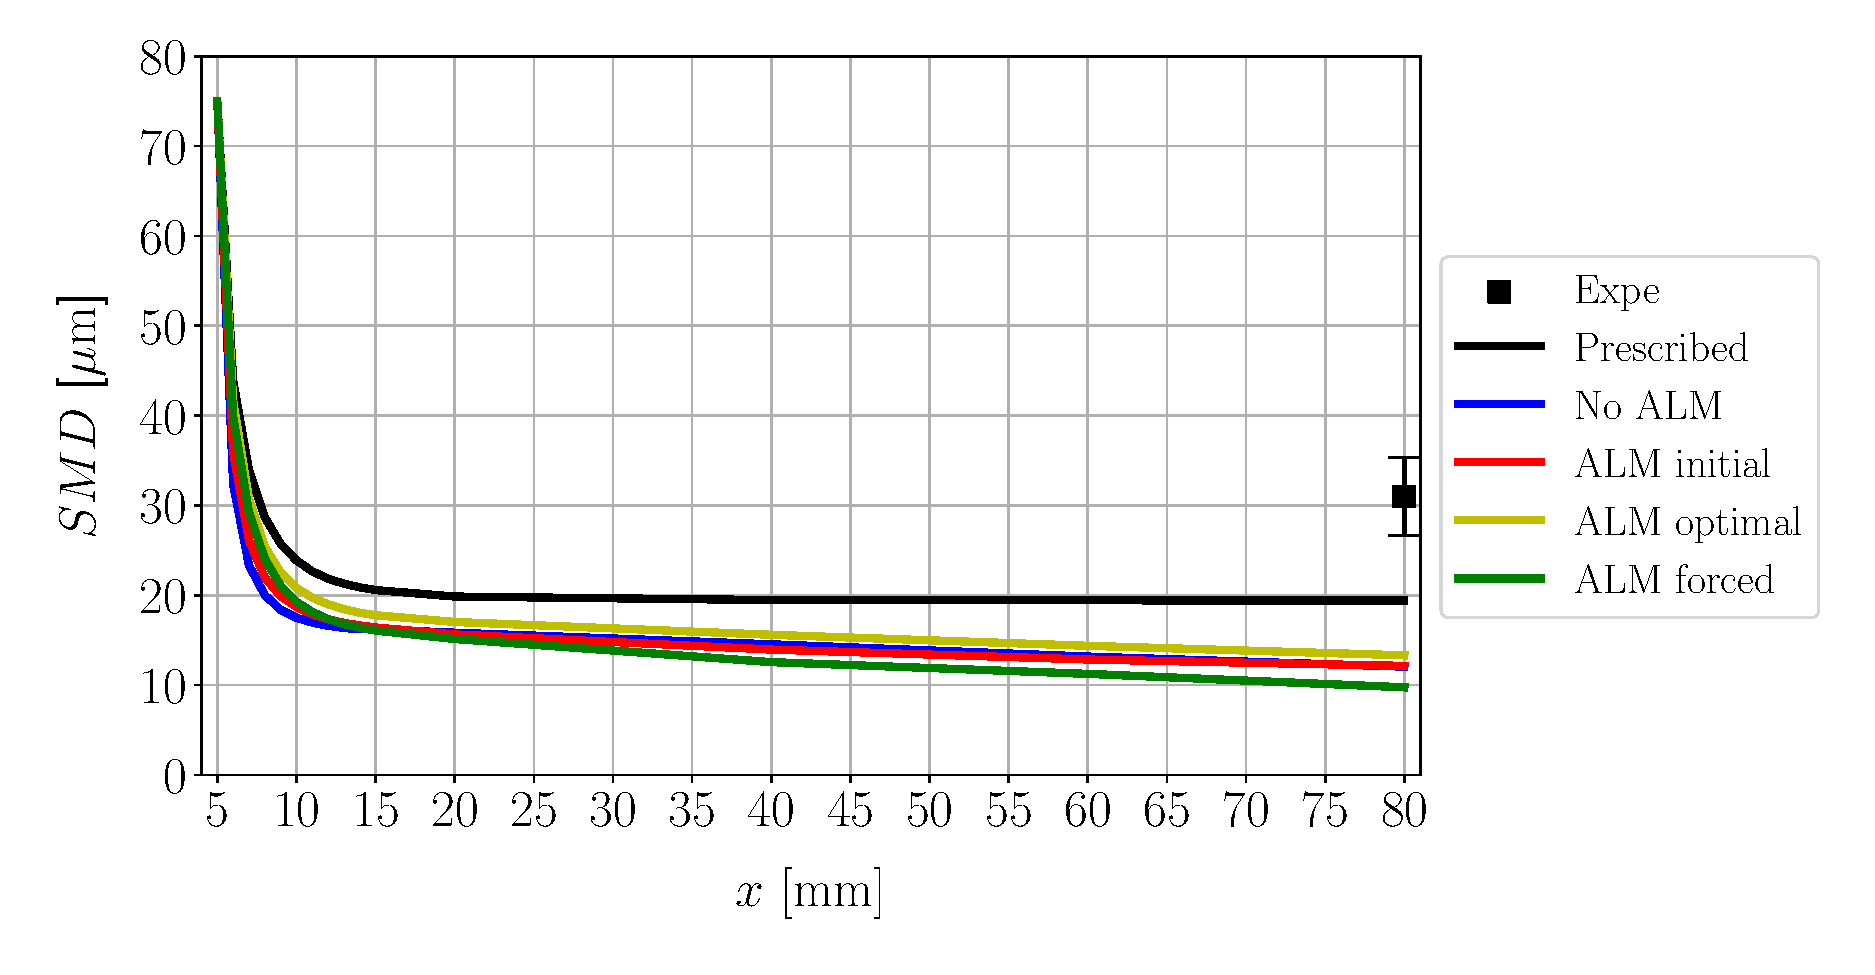
\includegraphics[scale=0.5]{./part2_developments/figures_ch6_lagrangian_JICF/params_gaseous_initial_conditions/SMD_vs_x_gaseous_BCs_comparison}
\caption[Evolution of SMD along axial location $x$ for the different gaseous boundary conditions tested]{Evolution of SMD along axial location $x$ for the different gaseous boundary conditions tested. The SMD at $x = 5$ and $10$ mm for the resolved atomization case UG100\_DX10 is also added for comparison}
\label{fig:SMD_vs_x_param_gaseous_BCs}
\end{figure}


\subsubsection*{Experimental comparison}

For validating the numerical simulations, the sprays from those are processed at $x = 80$ mm and compared with the available experimental data at this location. In first place, the $SMD$ and volume flux $q_l$ maps are shown in Figure \ref{fig:maps_LGS_JICF_gaseous_influence}. The experimental maps from Figure \ref{fig:maps_Becker_expe_results} are also displayed: the SMD scale has been changed in order to allow for a visual comparison with the simulation results. 



Eqs. (\ref{eq:integrated_results_Becker_expe_results}) have been applied to the simulations performed in order to obtain spatial-averaged contours of flux and SMD. The numerical results are compared to the experimental ones from Figure \ref{fig:integrated_results_Becker_expe_results} for the high Weber case.

In order to 

In first place, the evolution of the SMD



\clearpage

%\subsection{Vertical trajectories of lagrangian sprays}

\begin{figure}[h!]
\flushleft
\begin{subfigure}[b]{0.2\textwidth}
	\flushleft
%	\hspace*{-0.35in}
   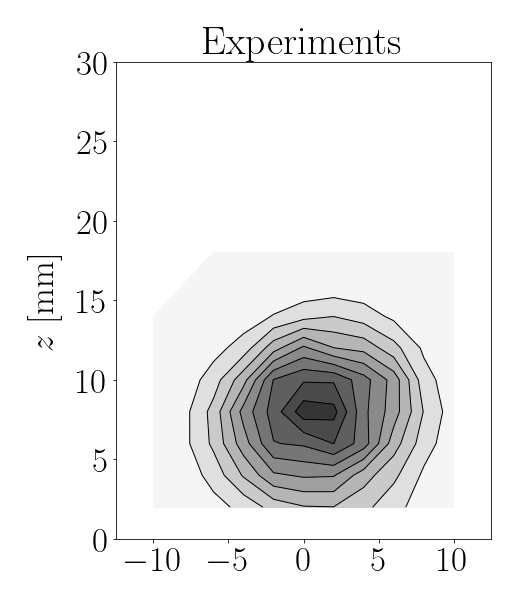
\includegraphics[scale=0.4]{./part2_developments/figures_ch6_lagrangian_JICF/params_gaseous_initial_conditions/maps/expe_flux}
   %\label{} 
\end{subfigure}
\hspace*{0.275in}
\begin{subfigure}[b]{0.2\textwidth}
	\flushleft
   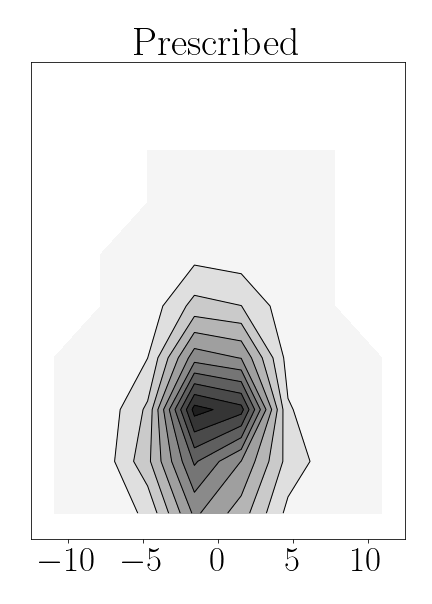
\includegraphics[scale=0.4]{./part2_developments/figures_ch6_lagrangian_JICF/params_gaseous_initial_conditions/maps/prescribed_flux}
   %\label{} 
\end{subfigure}
\hspace*{0.00in}
\begin{subfigure}[b]{0.2\textwidth}
	\flushleft
   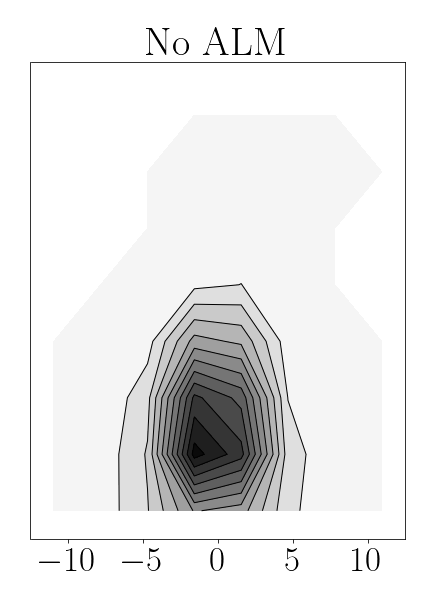
\includegraphics[scale=0.4]{./part2_developments/figures_ch6_lagrangian_JICF/params_gaseous_initial_conditions/maps/no_ALM_flux}
   %\label{} 
\end{subfigure}
\hspace*{0.00in}
\begin{subfigure}[b]{0.2\textwidth}
	\flushleft
   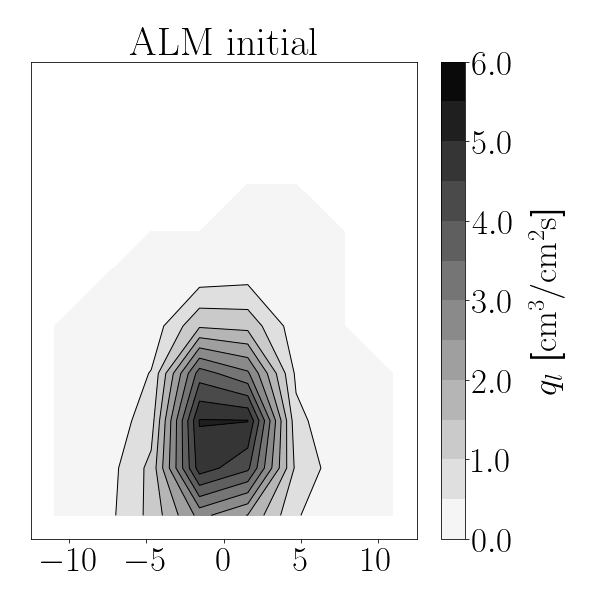
\includegraphics[scale=0.4]{./part2_developments/figures_ch6_lagrangian_JICF/params_gaseous_initial_conditions/maps/ALM_initial_flux}
   %\label{} 
\end{subfigure}

\vspace*{-0.25in}

\flushleft
\begin{subfigure}[b]{0.2\textwidth}
	\flushleft
%	\hspace*{-0.35in}
   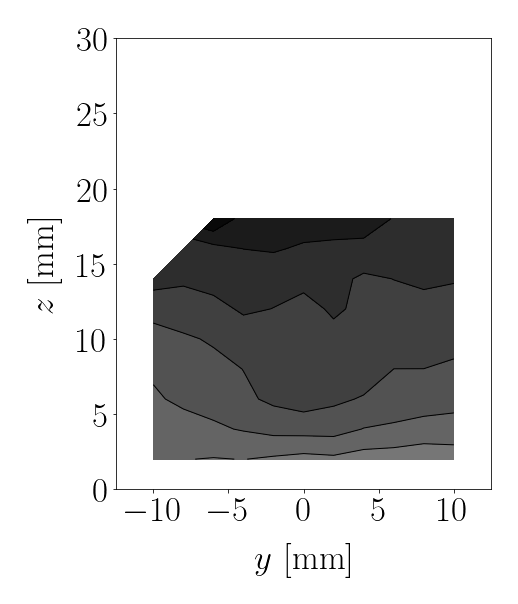
\includegraphics[scale=0.4]{./part2_developments/figures_ch6_lagrangian_JICF/params_gaseous_initial_conditions/maps/expe_SMD}
   %\label{} 
\end{subfigure}
\hspace*{0.25in}
\begin{subfigure}[b]{0.2\textwidth}
	\flushleft
   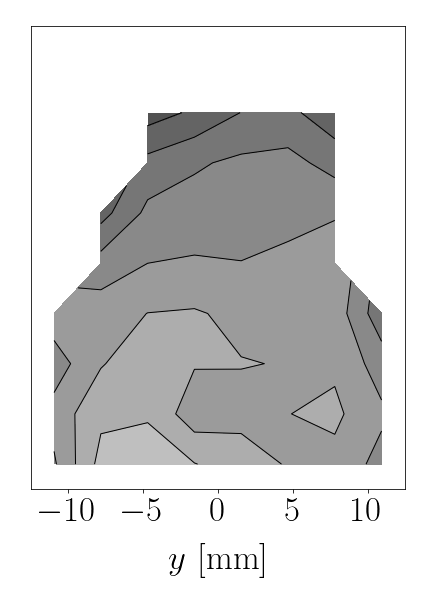
\includegraphics[scale=0.4]{./part2_developments/figures_ch6_lagrangian_JICF/params_gaseous_initial_conditions/maps/prescribed_SMD}
   %\label{} 
\end{subfigure}
\hspace*{0.00in}
\begin{subfigure}[b]{0.2\textwidth}
	\flushleft
   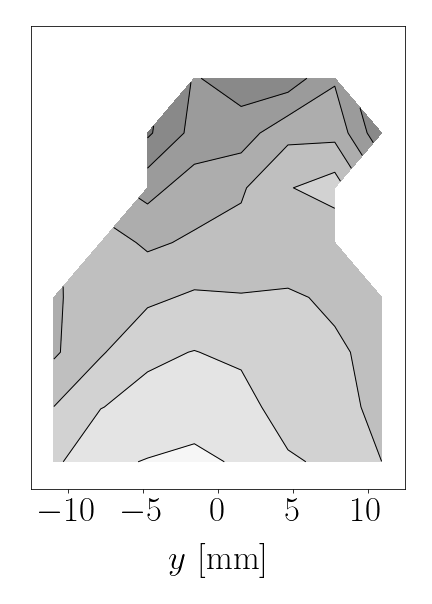
\includegraphics[scale=0.4]{./part2_developments/figures_ch6_lagrangian_JICF/params_gaseous_initial_conditions/maps/no_ALM_SMD}
   %\label{} 
\end{subfigure}
\hspace*{0.00in}
\begin{subfigure}[b]{0.2\textwidth}
	\flushleft
   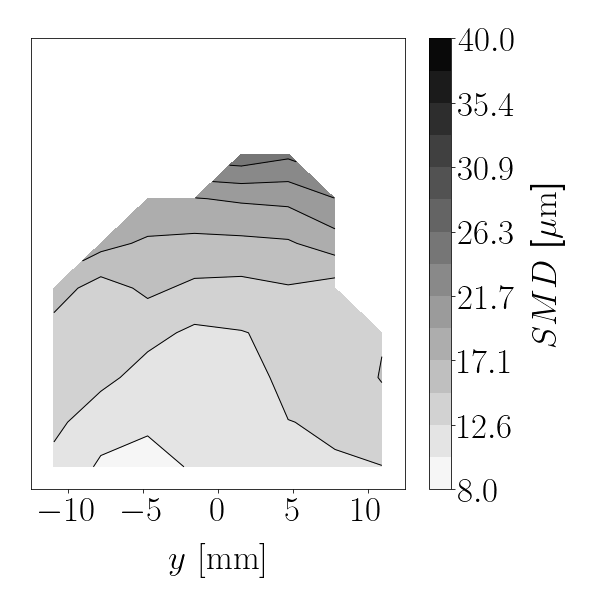
\includegraphics[scale=0.4]{./part2_developments/figures_ch6_lagrangian_JICF/params_gaseous_initial_conditions/maps/ALM_initial_SMD}
   %\label{} 
\end{subfigure}

\vskip\baselineskip

\begin{subfigure}[b]{0.2\textwidth}
	\flushleft
%	\hspace*{-0.35in}
   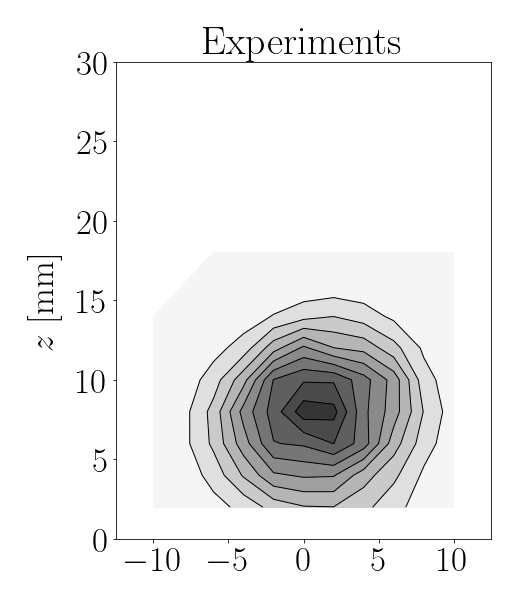
\includegraphics[scale=0.4]{./part2_developments/figures_ch6_lagrangian_JICF/params_gaseous_initial_conditions/maps/expe_flux}
   %\label{} 
\end{subfigure}
\hspace*{0.25in}
\begin{subfigure}[b]{0.2\textwidth}
	\flushleft
   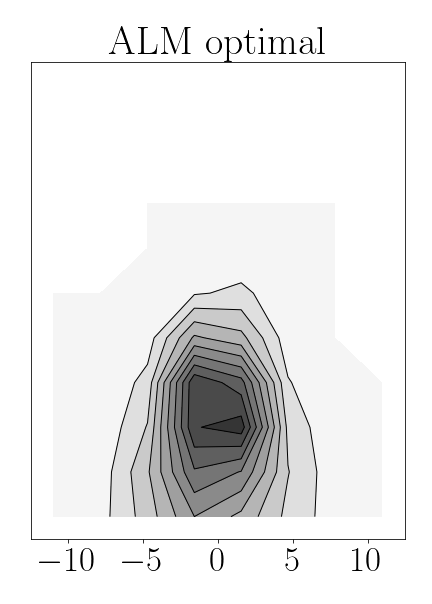
\includegraphics[scale=0.4]{./part2_developments/figures_ch6_lagrangian_JICF/params_gaseous_initial_conditions/maps/ALM_FDC_0p24_flux}
   %\label{} 
\end{subfigure}
\hspace*{0.00in}
\begin{subfigure}[b]{0.2\textwidth}
	\flushleft
   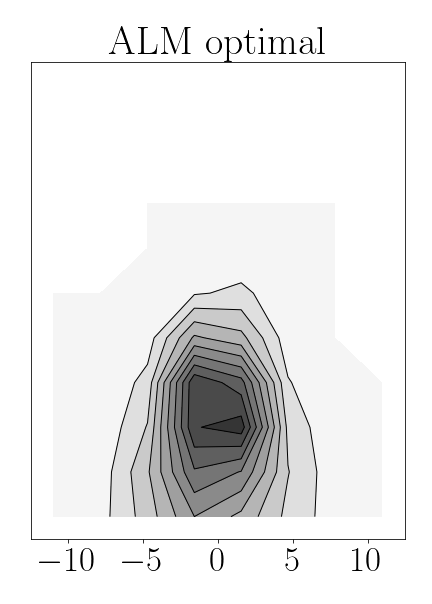
\includegraphics[scale=0.4]{./part2_developments/figures_ch6_lagrangian_JICF/params_gaseous_initial_conditions/maps/ALM_FDC_0p24_flux}
   %\label{} 
\end{subfigure}
\hspace*{0.00in}
\begin{subfigure}[b]{0.2\textwidth}
	\flushleft
   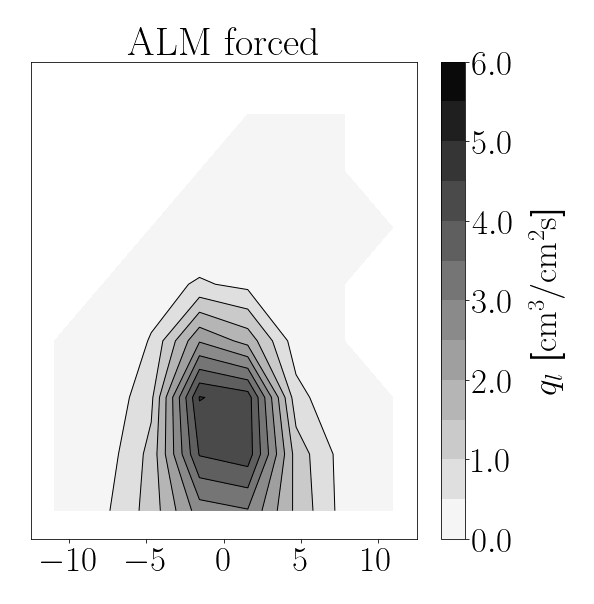
\includegraphics[scale=0.4]{./part2_developments/figures_ch6_lagrangian_JICF/params_gaseous_initial_conditions/maps/ALM_FDC_0p30_flux}
   %\label{} 
\end{subfigure}

\vspace*{-0.25in}

\flushleft
\begin{subfigure}[b]{0.2\textwidth}
	\flushleft
%	\hspace*{-0.35in}
   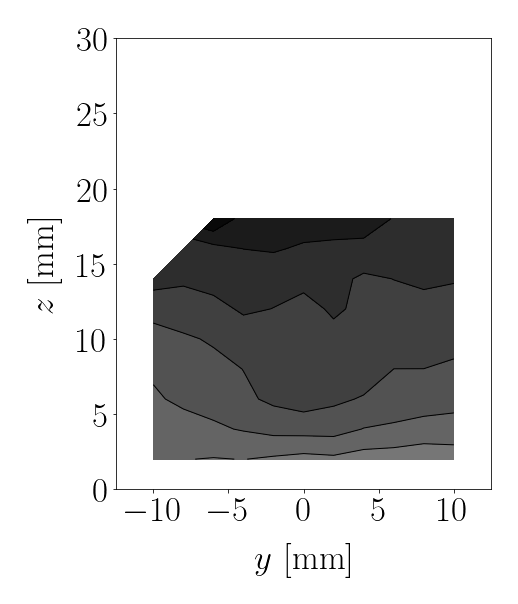
\includegraphics[scale=0.4]{./part2_developments/figures_ch6_lagrangian_JICF/params_gaseous_initial_conditions/maps/expe_SMD}
   %\label{} 
\end{subfigure}
\hspace*{0.25in}
\begin{subfigure}[b]{0.2\textwidth}
	\flushleft
   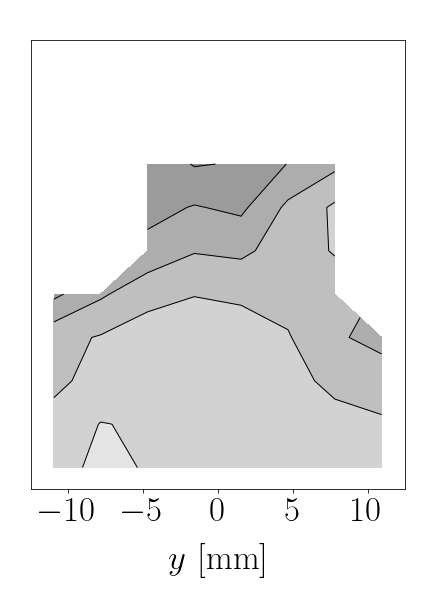
\includegraphics[scale=0.4]{./part2_developments/figures_ch6_lagrangian_JICF/params_gaseous_initial_conditions/maps/ALM_FDC_0p24_SMD}
   %\label{} 
\end{subfigure}
\hspace*{0.00in}
\begin{subfigure}[b]{0.2\textwidth}
	\flushleft
   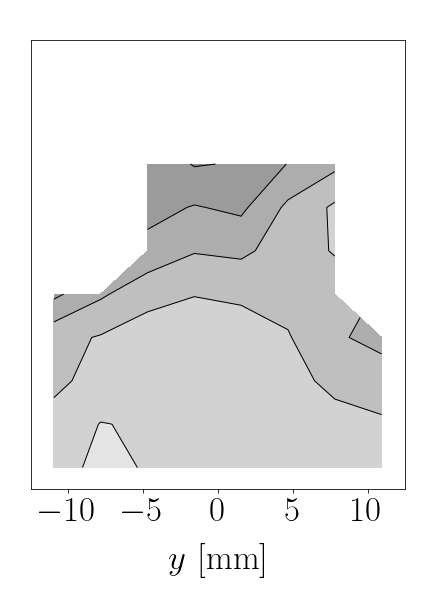
\includegraphics[scale=0.4]{./part2_developments/figures_ch6_lagrangian_JICF/params_gaseous_initial_conditions/maps/ALM_FDC_0p24_SMD}
   %\label{} 
\end{subfigure}
\hspace*{0.00in}
\begin{subfigure}[b]{0.2\textwidth}
	\flushleft
   \includegraphics[scale=0.4]{./part2_developments/figures_ch6_lagrangian_JICF/params_gaseous_initial_conditions/maps/ALM_FDC_0p30_SMD}
   %\label{} 
\end{subfigure}

\caption{Flux and SMD maps for numerical simulations comparing the effect of gaseous phase modelling with the experimental results}
\label{fig:maps_LGS_JICF_gaseous_influence}
\end{figure}














\clearpage



\begin{figure}[h!]
\flushleft
\begin{subfigure}[b]{0.2\textwidth}
	\flushleft
   \includegraphics[scale=0.35]{./part2_developments/figures_ch6_lagrangian_JICF/params_gaseous_initial_conditions/profiles/flux_along_z}
   %\label{} 
\end{subfigure}
\hspace*{0.5in}
\begin{subfigure}[b]{0.2\textwidth}
	\flushleft
   \includegraphics[scale=0.35]{./part2_developments/figures_ch6_lagrangian_JICF/params_gaseous_initial_conditions/profiles/SMD_along_z}
   %\label{} 
\end{subfigure}
\hspace*{0.1in}
\begin{subfigure}[b]{0.4\textwidth}
	\flushleft
   \includegraphics[scale=0.35]{./part2_developments/figures_ch6_lagrangian_JICF/params_gaseous_initial_conditions/profiles/flux_along_y}\\
   \vspace{-0.16in}
   \includegraphics[scale=0.35]{./part2_developments/figures_ch6_lagrangian_JICF/params_gaseous_initial_conditions/profiles/SMD_along_y}
   %\label{} 
\end{subfigure}

\caption{Integrated profiles of flux and SMD maps for numerical simulations comparing the effect of gaseous phase modelling with the experimental results}
\label{fig:profiles_LGS_JICF_gaseous_influence}
\end{figure}


%\subsection{Frequential analysis}


\section{Influence of secondary atomization model}
\label{sec:SLI_LGS_secondary_breakup_models}

To consider the secondary breakup of lagrangian droplets in dispersed-phase simulations, three atomization models are available ($\S$\ref{sec:ch4_secondary_atomization_modeling}): TAB, ETAB and Gorokhovski. All these models estimate breakup according to the Weber based on the relative velocity, which is the known parameter to control secondary atomization. Then, the exact instant of breakup and the size and number of children droplets are calculated differently by each model. The TAB and ETAB models belong to the same family and provide fixed values for the parameters controlling the model, while the Gorokhovski's stochastic model presents two constants ($K_1, K_2$) that are to be calibrated by the user. Therefore, first in this section firstly the Gorokhovski's stochastic model is calibrated in order to better match the experimental results, as it has been previously done in other works using the same model \citemColor[apte_les_2003,senoner_simulation_2010].  Then, the best configuration obtained is compared to the results from the TAB and ETAB models. It is found that these models provide good results in terms of flux distribution but that greatly underestimate the droplets sizes after atomization, while in the Gorokhovski model the two control variables can be tuner in order to get a better tradeoff between the droplets sizes and fluxes distribution.

\subsection{Calibration of Gorokhovski model}
\label{subsec:second_atom_goro_calibration}

The Gorokhovski stochatic model, described in $\S$\ref{subsec:ch4_goro_model}, presents two free constants $K_1$ and $K_2$ in Eq. (\ref{eq:gorokhovski_epsilon_parameters_definition}) which can be tuned for each particular case and which affect the size of the children droplets produced.  The constant $K_1$ affects the mean value of the generated children particles a breakup event, while $K_2$ controls the deviation from this mean \citepColor[senoner_simulation_2010]. The tested values for these constants are summarized in Table \ref{tab:lgs_DoE_goro_constants}. Three values for $K_1$ and three for $K_2$ have been tested, making a total of 9 simulations performed. 

%\begin{table}[!h]
%\centering
%\caption{Design of experiments to assess the influence of constants $K_1,K_2$ from Gorokhovski stochastic model}
%\begin{tabular}{ccc}
%\thickhline
%\textbf{Case} & $K_1$ & $K_2$  \\
%\thickhline
%G11 & \multirow{3}{*}{ 0.05} & 0.1 \\
%G12 &  & 0.5 \\
%G13 & 1.0 \\
%\hline
%G11 & \multirow{3}{*}{ 0.1} & 0.1 \\
%G12 &  & 0.5 \\
%G13 & 1.0 \\
%\hline
%G11 & \multirow{3}{*}{ 0.2} & 0.1 \\
%G12 &  & 0.5 \\
%G13 & 1.0 \\
%\thickhline
%\end{tabular}
%\label{tab:lgs_DoE_goro_constants}
%\end{table}


\begin{table}[!h]
\centering
\caption{Design of experiments to assess the influence of constants $K_1,K_2$ from Gorokhovski stochastic model}
\begin{tabular}{cccccccccc}
\thickhline
%\textbf{Case} & & & & & & & &  & \\
%\thickhline
%$K_1$ & \multicolumn{3}{c}{0.05} & \multicolumn{3}{c}{0.1} & \multicolumn{3}{c}{0.2} \\  
$K_1$ & 0.05 & 0.05 & 0.05 & 0.1 & 0.1 & 0.1 & 0.2 & 0.2 & 0.2 \\  
$K_2$ & 0.1 & 0.5 & 1.0 & 0.1 & 0.5 & 1.0 & 0.1 & 0.5 & 1.0 \\
\thickhline
\end{tabular}
\label{tab:lgs_DoE_goro_constants}
\end{table}

In first place, the effect of the constant $K_1$ is assessed by varying it with a fixed valued $K_2 = 1.0$. 


In first place, the value of the constant $K_2$ is assessed by fixing the  value of the other constant to $K_1 = 0.1$. 

\begin{figure}[h!]
\centering
\includegraphics[scale=0.5]{./part2_developments/figures_ch6_lagrangian_JICF/apte_model_calibration_u_vw_lognorm/SMD_vs_x_apte_calibration_comparison}
\caption[Evolution of SMD along axial location $x$ for several values of the Gorokhovski atomization model]{Evolution of SMD along axial location $x$ for several values of constants $K_1$, $K_2$ of the Gorokhovski atomization model. The SMD at $x = 5$ and $10$ mm for the resolved atomization case UG100\_DX10 is also added for comparison}
\label{fig:SMD_vs_x_param_breakup_model}
\end{figure}

\clearpage



\begin{figure}[h!]
\flushleft
\begin{subfigure}[b]{0.2\textwidth}
	\flushleft
%	\hspace*{-0.35in}
   \includegraphics[scale=0.4]{./part2_developments/figures_ch6_lagrangian_JICF/apte_model_calibration_u_vw_lognorm/maps/expe_flux}
   %\label{} 
\end{subfigure}
\hspace*{0.27in}
\begin{subfigure}[b]{0.2\textwidth}
	\flushleft
   \includegraphics[scale=0.4]{./part2_developments/figures_ch6_lagrangian_JICF/apte_model_calibration_u_vw_lognorm/maps/k1_0p05_k2_1p0_flux}
   %\label{} 
\end{subfigure}
\hspace*{0.02in}
\begin{subfigure}[b]{0.2\textwidth}
	\flushleft
   \includegraphics[scale=0.4]{./part2_developments/figures_ch6_lagrangian_JICF/apte_model_calibration_u_vw_lognorm/maps/k1_0p10_k2_1p0_flux}
   %\label{} 
\end{subfigure}
\hspace*{0.02in}
\begin{subfigure}[b]{0.2\textwidth}
	\flushleft
   \includegraphics[scale=0.4]{./part2_developments/figures_ch6_lagrangian_JICF/apte_model_calibration_u_vw_lognorm/maps/k1_0p20_k2_1p0_flux}
   %\label{} 
\end{subfigure}

\vspace*{-0.25in}

\flushleft
\begin{subfigure}[b]{0.2\textwidth}
	\flushleft
%	\hspace*{-0.35in}
   \includegraphics[scale=0.4]{./part2_developments/figures_ch6_lagrangian_JICF/apte_model_calibration_u_vw_lognorm/maps/expe_SMD}
   %\label{} 
\end{subfigure}
\hspace*{0.27in}
\begin{subfigure}[b]{0.2\textwidth}
	\flushleft
   \includegraphics[scale=0.4]{./part2_developments/figures_ch6_lagrangian_JICF/apte_model_calibration_u_vw_lognorm/maps/k1_0p05_k2_1p0_SMD}
   %\label{} 
\end{subfigure}
\hspace*{0.02in}
\begin{subfigure}[b]{0.2\textwidth}
	\flushleft
   \includegraphics[scale=0.4]{./part2_developments/figures_ch6_lagrangian_JICF/apte_model_calibration_u_vw_lognorm/maps/k1_0p10_k2_1p0_SMD}
   %\label{} 
\end{subfigure}
\hspace*{0.02in}
\begin{subfigure}[b]{0.2\textwidth}
	\flushleft
   \includegraphics[scale=0.4]{./part2_developments/figures_ch6_lagrangian_JICF/apte_model_calibration_u_vw_lognorm/maps/k1_0p20_k2_1p0_SMD}
   %\label{} 
\end{subfigure}

\vskip\baselineskip
\begin{subfigure}[b]{0.2\textwidth}
	\flushleft
%	\hspace*{-0.35in}
   \includegraphics[scale=0.4]{./part2_developments/figures_ch6_lagrangian_JICF/apte_model_calibration_u_vw_lognorm/maps/expe_flux}
   %\label{} 
\end{subfigure}
\hspace*{0.27in}
\begin{subfigure}[b]{0.2\textwidth}
	\flushleft
   \includegraphics[scale=0.4]{./part2_developments/figures_ch6_lagrangian_JICF/apte_model_calibration_u_vw_lognorm/maps/k1_0p05_k2_0p1_flux}
   %\label{} 
\end{subfigure}
\hspace*{0.02in}
\begin{subfigure}[b]{0.2\textwidth}
	\flushleft
   \includegraphics[scale=0.4]{./part2_developments/figures_ch6_lagrangian_JICF/apte_model_calibration_u_vw_lognorm/maps/k1_0p05_k2_0p5_flux}
   %\label{} 
\end{subfigure}
\hspace*{0.02in}
\begin{subfigure}[b]{0.2\textwidth}
	\flushleft
   \includegraphics[scale=0.4]{./part2_developments/figures_ch6_lagrangian_JICF/apte_model_calibration_u_vw_lognorm/maps/k1_0p05_k2_1p0_flux}
   %\label{} 
\end{subfigure}

\vspace*{-0.25in}

\flushleft
\begin{subfigure}[b]{0.2\textwidth}
	\flushleft
%	\hspace*{-0.35in}
   \includegraphics[scale=0.4]{./part2_developments/figures_ch6_lagrangian_JICF/apte_model_calibration_u_vw_lognorm/maps/expe_SMD}
   %\label{} 
\end{subfigure}
\hspace*{0.27in}
\begin{subfigure}[b]{0.2\textwidth}
	\flushleft
   \includegraphics[scale=0.4]{./part2_developments/figures_ch6_lagrangian_JICF/apte_model_calibration_u_vw_lognorm/maps/k1_0p05_k2_0p1_SMD}
   %\label{} 
\end{subfigure}
\hspace*{0.02in}
\begin{subfigure}[b]{0.2\textwidth}
	\flushleft
   \includegraphics[scale=0.4]{./part2_developments/figures_ch6_lagrangian_JICF/apte_model_calibration_u_vw_lognorm/maps/k1_0p05_k2_0p5_SMD}
   %\label{} 
\end{subfigure}
\hspace*{0.02in}
\begin{subfigure}[b]{0.2\textwidth}
	\flushleft
   \includegraphics[scale=0.4]{./part2_developments/figures_ch6_lagrangian_JICF/apte_model_calibration_u_vw_lognorm/maps/k1_0p05_k2_1p0_SMD}
   %\label{} 
\end{subfigure}


\caption{Flux and SMD maps for numerical simulations comparing the effect of calibrating the constants from the Gorokhovski model with the experimental results}
\label{fig:maps_LGS_JICF_second_atom_apte_calibration}
\end{figure}






\clearpage

\begin{figure}[h!]
\flushleft
\begin{subfigure}[b]{0.2\textwidth}
	\flushleft
   \includegraphics[scale=0.35]{./part2_developments/figures_ch6_lagrangian_JICF/apte_model_calibration_u_vw_lognorm/profiles/flux_along_z}
   %\label{} 
\end{subfigure}
\hspace*{0.5in}
\begin{subfigure}[b]{0.2\textwidth}
	\flushleft
   \includegraphics[scale=0.35]{./part2_developments/figures_ch6_lagrangian_JICF/apte_model_calibration_u_vw_lognorm/profiles/SMD_along_z}
   %\label{} 
\end{subfigure}
\hspace*{0.1in}
\begin{subfigure}[b]{0.4\textwidth}
	\flushleft
   \includegraphics[scale=0.35]{./part2_developments/figures_ch6_lagrangian_JICF/apte_model_calibration_u_vw_lognorm/profiles/flux_along_y}\\
   \vspace{-0.16in}
   \includegraphics[scale=0.35]{./part2_developments/figures_ch6_lagrangian_JICF/apte_model_calibration_u_vw_lognorm/profiles/SMD_along_y}
   %\label{} 
\end{subfigure}

\caption{Integrated profiles of flux and SMD maps for numerical simulations comparing the effect of Gorokhovski's model calibration with the experimental results}
\label{fig:profiles_LGS_JICF_apte_calibration}
\end{figure}


\begin{table}[!h]
\centering
\caption{SMD values at $x = 80$ mm obtained with different constants in the Gorokhovski secondary atomization model}
\begin{tabular}{ccc}
\thickhline
Case & $SMD~\left[\mu \mathrm{m} \right]$ & $\varepsilon_{SMD}~\left[\% \right]$ \\
\thickhline
Experiments & 31 & - \\
$K_1 = 0.05,~K_2 = 0.1$ & 16.60 & -46.45 \\
$K_1 = 0.05,~K_2 = 0.5$ & 18.68 & -39.75 \\
$K_1 = 0.05,~K_2 = 1.0$ & 19.44 & -37.29 \\
$K_1 = 0.10,~K_2 = 1.0$ & 18.57 & -40.11 \\
$K_1 = 0.20,~K_2 = 1.0$ & 17.58 & -43.28 \\
\thickhline
\end{tabular}
\label{tab:SMD_deviations_turb_inj}
\end{table}

\clearpage


\subsection{Comparison of breakup models}

The evolution of SMD with axial distance is plotted in Figure \ref{fig:SMD_vs_x_param_breakup_model}.

The maps of SMD and liquid flux are shown in Figure \ref{fig:maps_LGS_JICF_second_atom_models}.

Figure \ref{fig:profiles_LGS_JICF_secondary_atom_model} shows the integrated flux and SMD profiles.

\begin{figure}[h!]
\centering
\includegraphics[scale=0.5]{./part2_developments/figures_ch6_lagrangian_JICF/params_breakup_model/SMD_vs_x_breakup_models_comparison}
\caption[Evolution of SMD along axial location $x$ for the three atomization models]{Evolution of SMD along axial location $x$ for the three atomization models. The SMD at $x = 5$ and $10$ mm for the resolved atomization case UG100\_DX10 is also added for comparison}
\label{fig:SMD_vs_x_param_breakup_model}
\end{figure}

\clearpage

\begin{figure}[h!]
\flushleft
\begin{subfigure}[b]{0.2\textwidth}
	\flushleft
%	\hspace*{-0.35in}
   \includegraphics[scale=0.4]{./part2_developments/figures_ch6_lagrangian_JICF/params_breakup_model/maps/expe_flux}
   %\label{} 
\end{subfigure}
\hspace*{0.27in}
\begin{subfigure}[b]{0.2\textwidth}
	\flushleft
   \includegraphics[scale=0.4]{./part2_developments/figures_ch6_lagrangian_JICF/params_breakup_model/maps/goro_flux}
   %\label{} 
\end{subfigure}
\hspace*{0.02in}
\begin{subfigure}[b]{0.2\textwidth}
	\flushleft
   \includegraphics[scale=0.4]{./part2_developments/figures_ch6_lagrangian_JICF/params_breakup_model/maps/TAB_flux}
   %\label{} 
\end{subfigure}
\hspace*{0.02in}
\begin{subfigure}[b]{0.2\textwidth}
	\flushleft
   \includegraphics[scale=0.4]{./part2_developments/figures_ch6_lagrangian_JICF/params_breakup_model/maps/ETAB_flux}
   %\label{} 
\end{subfigure}

\vspace*{-0.25in}

\flushleft
\begin{subfigure}[b]{0.2\textwidth}
	\flushleft
%	\hspace*{-0.35in}
   \includegraphics[scale=0.4]{./part2_developments/figures_ch6_lagrangian_JICF/params_breakup_model/maps/expe_SMD}
   %\label{} 
\end{subfigure}
\hspace*{0.27in}
\begin{subfigure}[b]{0.2\textwidth}
	\flushleft
   \includegraphics[scale=0.4]{./part2_developments/figures_ch6_lagrangian_JICF/params_breakup_model/maps/goro_SMD}
   %\label{} 
\end{subfigure}
\hspace*{0.02in}
\begin{subfigure}[b]{0.2\textwidth}
	\flushleft
   \includegraphics[scale=0.4]{./part2_developments/figures_ch6_lagrangian_JICF/params_breakup_model/maps/TAB_SMD}
   %\label{} 
\end{subfigure}
\hspace*{0.02in}
\begin{subfigure}[b]{0.2\textwidth}
	\flushleft
   \includegraphics[scale=0.4]{./part2_developments/figures_ch6_lagrangian_JICF/params_breakup_model/maps/ETAB_SMD}
   %\label{} 
\end{subfigure}



\caption{Flux and SMD maps for numerical simulations comparing the effect of secondary atomization models with the experimental results}
\label{fig:maps_LGS_JICF_second_atom_models}
\end{figure}

\begin{figure}[h!]
\flushleft
\begin{subfigure}[b]{0.2\textwidth}
	\flushleft
   \includegraphics[scale=0.35]{./part2_developments/figures_ch6_lagrangian_JICF/params_breakup_model/profiles/flux_along_z}
   %\label{} 
\end{subfigure}
\hspace*{0.5in}
\begin{subfigure}[b]{0.2\textwidth}
	\flushleft
   \includegraphics[scale=0.35]{./part2_developments/figures_ch6_lagrangian_JICF/params_breakup_model/profiles/SMD_along_z}
   %\label{} 
\end{subfigure}
\hspace*{0.1in}
\begin{subfigure}[b]{0.4\textwidth}
	\flushleft
   \includegraphics[scale=0.35]{./part2_developments/figures_ch6_lagrangian_JICF/params_breakup_model/profiles/flux_along_y}\\
   \vspace{-0.16in}
   \includegraphics[scale=0.35]{./part2_developments/figures_ch6_lagrangian_JICF/params_breakup_model/profiles/SMD_along_y}
   %\label{} 
\end{subfigure}

\caption{Integrated profiles of flux and SMD maps for numerical simulations comparing the effect of secondary atomization models with the experimental results}
\label{fig:profiles_LGS_JICF_secondary_atom_model}
\end{figure}

\clearpage

\begin{table}[!h]
\centering
\caption{SMD values at $x = 80$ mm for simulations with the different secondary atomization models}
\begin{tabular}{ccc}
\thickhline
Case & $SMD~\left[\mu \mathrm{m} \right]$ & $\varepsilon_{SMD}~\left[\% \right]$ \\
\thickhline
Experiments & 31 & - \\
Gorokhovski & 19.44 & -37.29 \\
TAB & 13.93 & -55.07 \\
ETAB & 17.49 & -43.59 \\
\thickhline
\end{tabular}
\label{tab:SMD_deviations_turb_inj}
\end{table}



\section{Influence of SLI variables}
\label{sec:effect_of_SLI_variables}

\subsection{Level-set resolution and injection location}
\label{subsec:SLI_LGS_resolution_and_injection_location}

\begin{figure}[h!]
\flushleft
\begin{subfigure}[b]{0.2\textwidth}
	\flushleft
   \includegraphics[scale=0.35]{./part2_developments/figures_ch6_lagrangian_JICF/params_resol_and_xInj/profiles/flux_along_z}
   %\label{} 
\end{subfigure}
\hspace*{0.5in}
\begin{subfigure}[b]{0.2\textwidth}
	\flushleft
   \includegraphics[scale=0.35]{./part2_developments/figures_ch6_lagrangian_JICF/params_resol_and_xInj/profiles/SMD_along_z}
   %\label{} 
\end{subfigure}
\hspace*{0.1in}
\begin{subfigure}[b]{0.4\textwidth}
	\flushleft
   \includegraphics[scale=0.35]{./part2_developments/figures_ch6_lagrangian_JICF/params_resol_and_xInj/profiles/flux_along_y}\\
   \vspace{-0.16in}
   \includegraphics[scale=0.35]{./part2_developments/figures_ch6_lagrangian_JICF/params_resol_and_xInj/profiles/SMD_along_y}
   %\label{} 
\end{subfigure}

\caption{Integrated profiles of flux and SMD maps for numerical simulations comparing the effect of SLIs obtained with different resolutions and at several injection locations with the experimental results}
\label{fig:profiles_LGS_JICF_resol_and_xInj}
\end{figure}

\clearpage

\subsection{Spray velocities}
\label{subsec:SLI_LGS_velocity_effects}

\subsubsection*{Arithmetic vs volume-weighted mean veloticies}

\subsubsection*{RMS mean velocities}


\begin{figure}[h!]
\flushleft
\begin{subfigure}[b]{0.2\textwidth}
	\flushleft
   \includegraphics[scale=0.35]{./part2_developments/figures_ch6_lagrangian_JICF/params_spray_velocities/profiles/flux_along_z}
   %\label{} 
\end{subfigure}
\hspace*{0.5in}
\begin{subfigure}[b]{0.2\textwidth}
	\flushleft
   \includegraphics[scale=0.35]{./part2_developments/figures_ch6_lagrangian_JICF/params_spray_velocities/profiles/SMD_along_z}
   %\label{} 
\end{subfigure}
\hspace*{0.1in}
\begin{subfigure}[b]{0.4\textwidth}
	\flushleft
   \includegraphics[scale=0.35]{./part2_developments/figures_ch6_lagrangian_JICF/params_spray_velocities/profiles/flux_along_y}\\
   \vspace{-0.16in}
   \includegraphics[scale=0.35]{./part2_developments/figures_ch6_lagrangian_JICF/params_spray_velocities/profiles/SMD_along_y}
   %\label{} 
\end{subfigure}

\caption{Integrated profiles of flux and SMD maps for numerical simulations comparing the effect of spray velocities with the experimental results}
\label{fig:profiles_LGS_JICF_spray_velocities}
\end{figure}

\clearpage

\subsection{Droplets diameters}

\begin{figure}[h!]
\flushleft
\begin{subfigure}[b]{0.2\textwidth}
	\flushleft
   \includegraphics[scale=0.35]{./part2_developments/figures_ch6_lagrangian_JICF/params_f0/profiles/flux_along_z}
   %\label{} 
\end{subfigure}
\hspace*{0.5in}
\begin{subfigure}[b]{0.2\textwidth}
	\flushleft
   \includegraphics[scale=0.35]{./part2_developments/figures_ch6_lagrangian_JICF/params_f0/profiles/SMD_along_z}
   %\label{} 
\end{subfigure}
\hspace*{0.1in}
\begin{subfigure}[b]{0.4\textwidth}
	\flushleft
   \includegraphics[scale=0.35]{./part2_developments/figures_ch6_lagrangian_JICF/params_f0/profiles/flux_along_y}\\
   \vspace{-0.16in}
   \includegraphics[scale=0.35]{./part2_developments/figures_ch6_lagrangian_JICF/params_f0/profiles/SMD_along_y}
   %\label{} 
\end{subfigure}

\caption{Integrated profiles of flux and SMD maps for numerical simulations comparing the effect of injection diameters $f_0 \left( D \right)$ turbulence with the experimental results}
\label{fig:profiles_LGS_JICF_f0}
\end{figure}

\begin{table}[!h]
\centering
\caption{SMD values at $x = 80$ mm for simulations with and without turbulence injection}
\begin{tabular}{ccc}
\thickhline
Case & $SMD~\left[\mu \mathrm{m} \right]$ & $\varepsilon_{SMD}~\left[\% \right]$ \\
\thickhline
Experiments & 31 & - \\
LN & 19.71 & -36.42 \\
Constant & & \\
\thickhline
\end{tabular}
\label{tab:SMD_deviations_f0}
\end{table}


\clearpage


%\subsection{Droplets diameters WITH ETAB}
%
%\begin{figure}[h!]
%\flushleft
%\begin{subfigure}[b]{0.2\textwidth}
%	\flushleft
%   \includegraphics[scale=0.35]{./part2_developments/figures_ch6_lagrangian_JICF/params_f0/profiles_ETAB/flux_along_z}
%   %\label{} 
%\end{subfigure}
%\hspace*{0.5in}
%\begin{subfigure}[b]{0.2\textwidth}
%	\flushleft
%   \includegraphics[scale=0.35]{./part2_developments/figures_ch6_lagrangian_JICF/params_f0/profiles_ETAB/SMD_along_z}
%   %\label{} 
%\end{subfigure}
%\hspace*{0.1in}
%\begin{subfigure}[b]{0.4\textwidth}
%	\flushleft
%   \includegraphics[scale=0.35]{./part2_developments/figures_ch6_lagrangian_JICF/params_f0/profiles_ETAB/flux_along_y}\\
%   \vspace{-0.16in}
%   \includegraphics[scale=0.35]{./part2_developments/figures_ch6_lagrangian_JICF/params_f0/profiles_ETAB/SMD_along_y}
%   %\label{} 
%\end{subfigure}
%
%\caption{Integrated profiles of flux and SMD maps for numerical simulations comparing the effect of injection diameters $f_0 \left( D \right)$ turbulence with the experimental results}
%\label{fig:profiles_LGS_JICF_f0_ETAB}
%\end{figure}
%
%\begin{table}[!h]
%\centering
%\caption{SMD values at $x = 80$ mm for simulations with and without turbulence injection}
%\begin{tabular}{ccc}
%\thickhline
%Case & $SMD~\left[\mu \mathrm{m} \right]$ & $\varepsilon_{SMD}~\left[\% \right]$ \\
%\thickhline
%Experiments & 31 & - \\
%LN & 17.49 & -43.59 \\
%Constant & 17.47 & -43.66 \\
%\thickhline
%\end{tabular}
%\label{tab:SMD_deviations_f0_ETAB}
%\end{table}
%
%
%\clearpage


\subsection{Turbulence injection}

The effect of synthetic turbulence at the inlet is assessed by injecting droplets with the SLI obtained from simulation UG100\_DX10\_NT at $x = 5$ mm (Figure \ref{fig:injectors_SLI_extra_UG100_DX10_x05}) in a channel where data from the same simulation is extracted and prescribed at the inlet through Eq. (\ref{eq:prescribed_inlet_u_gas_injection_law}). Results at $x = 80$ mm from the dispersed-phase simulation are shown in Figure \ref{fig:profiles_LGS_JICF_turbulence_injection}. By substracting turbulence, secondary atomization is less agressive and the size of the droplets is larger, resulting in SMD profiles closer to experimentas values in both lateral and vertical directions and in a larger global SMD as shown in Table \ref{tab:SMD_deviations_turb_inj}. This influence of turbulence in breakup is expected, since it is known that a larger turbulent content enhances atomization \citepColor[reitz_modeling_1987]. Regarding flux, the vertical profile from Figure \ref{fig:profiles_LGS_JICF_turbulence_injection} shows larger liquid content in the bottom part of the spray and an underestimated vertical location of the maximum flux location. The 

\begin{figure}[h!]
\flushleft
\begin{subfigure}[b]{0.2\textwidth}
	\flushleft
   \includegraphics[scale=0.35]{./part2_developments/figures_ch6_lagrangian_JICF/params_turb_injection/profiles/flux_along_z}
   %\label{} 
\end{subfigure}
\hspace*{0.5in}
\begin{subfigure}[b]{0.2\textwidth}
	\flushleft
   \includegraphics[scale=0.35]{./part2_developments/figures_ch6_lagrangian_JICF/params_turb_injection/profiles/SMD_along_z}
   %\label{} 
\end{subfigure}
\hspace*{0.1in}
\begin{subfigure}[b]{0.4\textwidth}
	\flushleft
   \includegraphics[scale=0.35]{./part2_developments/figures_ch6_lagrangian_JICF/params_turb_injection/profiles/flux_along_y}\\
   \vspace{-0.16in}
   \includegraphics[scale=0.35]{./part2_developments/figures_ch6_lagrangian_JICF/params_turb_injection/profiles/SMD_along_y}
   %\label{} 
\end{subfigure}

\caption{Integrated profiles of flux and SMD maps for numerical simulations comparing the effect of injecting synthetic turbulence with the experimental results}
\label{fig:profiles_LGS_JICF_turbulence_injection}
\end{figure}

\begin{table}[!h]
\centering
\caption{SMD values at $x = 80$ mm for simulations with and without turbulence injection}
\begin{tabular}{ccc}
\thickhline
Case & $SMD~\left[\mu \mathrm{m} \right]$ & $\varepsilon_{SMD}~\left[\% \right]$ \\
\thickhline
Experiments & 31 & - \\
With turb. & 21.58 & -30.38 \\
Without turb. & 21.94 & -29.22 \\
\thickhline
\end{tabular}
\label{tab:SMD_deviations_turb_inj}
\end{table}

\clearpage

\subsection{Convergence-driven discretization}

The use of convergence-driven discretization through quadtrees is assessed by performing a simulation with the SLI injectors shown in Figure \hl{\textbf{XX}}. Results for the spatially-integrated profiles of flux and SMD at $x = 80$ mm  are shown in Figure \ref{fig:profiles_LGS_JICF_quadtrees}. As observed, by using finer discretized injectors the vertical penetration of the spray is lower, being closer to the experimental limits. The maximum fuel flux location in the vertical direction is  shifted upwards when compared to the case without quadtrees, hence being slightly overestimated but still close to the experimental location. The SMD values are also affected by the quadtrees: droplets are smaller when these are used, hence the SMD profiles are underestimated in both vertical and lateral directions. \hl{Such reduction in SMD with convergence-driven discretization might be due to ...}. SMD underestimation is also reflected in the global SMD of the spray shown in Figure \ref{tab:SMD_deviations_quadtrees}, which as observed is lower when convergence-driven discretization is used and therefore yields a larger error when compared to the experimental value.



\begin{figure}[h!]
\flushleft
\begin{subfigure}[b]{0.2\textwidth}
	\flushleft
   \includegraphics[scale=0.35]{./part2_developments/figures_ch6_lagrangian_JICF/params_quadtrees/profiles/flux_along_z}
   %\label{} 
\end{subfigure}
\hspace*{0.5in}
\begin{subfigure}[b]{0.2\textwidth}
	\flushleft
   \includegraphics[scale=0.35]{./part2_developments/figures_ch6_lagrangian_JICF/params_quadtrees/profiles/SMD_along_z}
   %\label{} 
\end{subfigure}
\hspace*{0.1in}
\begin{subfigure}[b]{0.4\textwidth}
	\flushleft
   \includegraphics[scale=0.35]{./part2_developments/figures_ch6_lagrangian_JICF/params_quadtrees/profiles/flux_along_y}\\
   \vspace{-0.16in}
   \includegraphics[scale=0.35]{./part2_developments/figures_ch6_lagrangian_JICF/params_quadtrees/profiles/SMD_along_y}
   %\label{} 
\end{subfigure}

\caption{Integrated profiles of flux and SMD maps for numerical simulations comparing the effect of convergence-driven discretization with quadtrees with the experimental results}
\label{fig:profiles_LGS_JICF_quadtrees}
\end{figure}

The SMD of the sprays at $x = 80$ mm are shown at Table \ref{tab:SMD_deviations_quadtrees}. 

\begin{table}[!h]
\centering
\caption{SMD values at $x = 80$ mm for simulations with and without quadtrees}
\begin{tabular}{ccc}
\thickhline
Case & $SMD~\left[\mu \mathrm{m} \right]$ & $\varepsilon_{SMD}~\left[\% \right]$ \\
\thickhline
Experiments & 31 & - \\
Without quadtrees & 19.44 & - 37.29 \\
With quadtrees & 16.60 & - 46.44 \\
\thickhline
\end{tabular}
\label{tab:SMD_deviations_quadtrees}
\end{table}

\clearpage

\subsection{Operating condition}


\clearpage

\section{Delay in secondary atomization}

\begin{figure}[h!]
\centering
\includegraphics[scale=0.5]{./part2_developments/figures_ch6_lagrangian_JICF/params_dx_atom/SMD_vs_x_dx_atom_comparison}
\caption[Evolution of SMD along axial location $x$ with parameter $\Delta x_\mathrm{atom}$]{Evolution of SMD along axial location $x$ with parameter $\Delta x_\mathrm{atom}$}
\label{fig:SMD_vs_x_param_dx_atom}
\end{figure}

\begin{figure}[h!]
\flushleft
\begin{subfigure}[b]{0.2\textwidth}
	\flushleft
   \includegraphics[scale=0.35]{./part2_developments/figures_ch6_lagrangian_JICF/params_dx_atom/profiles/flux_along_z}
   %\label{} 
\end{subfigure}
\hspace*{0.5in}
\begin{subfigure}[b]{0.2\textwidth}
	\flushleft
   \includegraphics[scale=0.35]{./part2_developments/figures_ch6_lagrangian_JICF/params_dx_atom/profiles/SMD_along_z}
   %\label{} 
\end{subfigure}
\hspace*{0.1in}
\begin{subfigure}[b]{0.4\textwidth}
	\flushleft
   \includegraphics[scale=0.35]{./part2_developments/figures_ch6_lagrangian_JICF/params_dx_atom/profiles/flux_along_y}\\
   \vspace{-0.16in}
   \includegraphics[scale=0.35]{./part2_developments/figures_ch6_lagrangian_JICF/params_dx_atom/profiles/SMD_along_y}
   %\label{} 
\end{subfigure}

\caption{Integrated profiles of flux and SMD maps for numerical simulations comparing the effect of $\Delta x_\mathrm{atom}$ with the experimental results}
\label{fig:profiles_LGS_JICF_secondary_atom_model}
\end{figure}



\begin{figure}[h!]
\centering
\includegraphics[scale=0.5]{./part2_developments/figures_ch6_lagrangian_JICF/params_dx_atom/SMD_vs_dx_atom}
\caption{SMD at $x = 80$ mm for several values of parameter $\Delta x_\mathrm{atom}$ }
\label{fig:SMD_vs_dx_atom}
\end{figure}

\clearpage

\section{Computational costs}

\section{Conclusions}





